%input macros (i.e. write your own macros file called MacroFile1.tex)
%\newcommand{\PdfPsText}[2]{
  \ifpdf
     #1
  \else
     #2
  \fi
}

\newcommand{\IncludeGraphicsH}[3]{
  \PdfPsText{\includegraphics[height=#2]{#1}}{\includegraphics[bb = #3, height=#2]{#1}}
}

\newcommand{\IncludeGraphicsW}[3]{
  \PdfPsText{\includegraphics[width=#2]{#1}}{\includegraphics[bb = #3, width=#2]{#1}}
}

\newcommand{\InsertFig}[3]{
  \begin{figure}[!htbp]
    \begin{center}
      \leavevmode
      #1
      \caption{#2}
      \label{#3}
    \end{center}
  \end{figure}
}


%%% Local Variables: 
%%% mode: latex
%%% TeX-master: "~/Documents/LaTeX/CUEDThesisPSnPDF/thesis"
%%% End: 


 \documentclass[oneside,12pt]{Classes/CUEDthesisPSnPDF}


\ifpdf
    \pdfinfo { /Title  (Tag Clouds in Software Visualisation)
               /Creator (TeX)
               /Producer (pdfTeX)
               /Author (Jessica Emerson jmt.emerson@gmail.com)
               /CreationDate (D:20030101000000)  %format D:YYYYMMDDhhmmss
               /ModDate (D:20030815213532)
               /Subject (Tag Clouds in Software Visualisation)
               /Keywords (Word Clouds, Tag Clouds, Software Visualisation, Thesis)}
    \pdfcatalog { /PageMode (/UseOutlines)
                  /OpenAction (fitbh)  }
\fi

\title{Tag Clouds in Software Visualisation}

\ifpdf
  \author{\href{mailto:jmt.emerson@gmail.com}{Jessica Emerson}}
  \collegeordept{\href{http://www.cosc.canterbury.ac.nz/}{Department of Computer Science and Software Engineering}}
  \university{\href{http://www.canterbury.ac.nz/}{University of Canterbury}}
% insert below the file name that contains the crest in-place of 'UnivShield'
  \crest{\includegraphics[width=60mm]{UCLogo}}
\else
  \author{Jessica Emerson}
  \collegeordept{Department of Computer Science and Software Engineering}
  \university{University of Canterbury}
% insert below the file name that contains the crest in-place of 'UnivShield'
  \crest{\includegraphics[bb = 0 0 292 336, width=30mm]{UCLogo}}
\fi
%
% insert below the file name that contains the crest in-place of 'UnivShield'
%\crest{\IncludeGraphicsW{UCLogo}{40mm}{14 14 73 81}}

%\renewcommand{\submittedtext}{change the default text here if needed}
\degree{Master of Science}
\degreedate{2014}

% turn of those nasty overfull and underfull hboxes
\hbadness=10000
\hfuzz=50pt

% Put all the style files you want in the directory StyleFiles and usepackage like this:
\usepackage{StyleFiles/watermark}


% Comment out the next line to get single spacing
\onehalfspacing

\begin{document}

%\language{english}

% A page with the abstract on including title and author etc may be
% required to be handed in separately. If this is not so, then comment
% the below 3 lines (between '\begin{abstractseparte}' and 
% 'end{abstractseparate}'), normally like a declaration ... needs some more
% work, mind as environment abstracts creates a new page!
% \begin{abstractseparate}
%   
% Thesis Abstract -----------------------------------------------------


%\begin{abstractslong}    %uncommenting this line, gives a different abstract heading
\begin{abstracts}        %this creates the heading for the abstract page

This is where you write your abstract ...


\end{abstracts}
%\end{abstractlongs}


% ----------------------------------------------------------------------


%%% Local Variables: 
%%% mode: latex
%%% TeX-master: "../thesis"
%%% End: 

% \end{abstractseparate}


% Using the watermark package which is in StyleFiles/
% and to remove DRAFT COPY ONLY appearing on the top of all pages comment out below line
%\watermark{DRAFT COPY ONLY}

\maketitle

%set the number of sectioning levels that get number and appear in the contents
\setcounter{secnumdepth}{3}
\setcounter{tocdepth}{3}

\frontmatter % book mode only
\pagenumbering{roman}
%% Thesis Dedictation ---------------------------------------------------

\begin{dedication} %this creates the heading for the dedication page

I would like to dedicate this thesis to my loving parents ...

\end{dedication}

% ----------------------------------------------------------------------

%%% Local Variables: 
%%% mode: latex
%%% TeX-master: "../thesis"
%%% End: 

%% Thesis Acknowledgements ------------------------------------------------


%\begin{acknowledgementslong} %uncommenting this line, gives a different acknowledgements heading
\begin{acknowledgements}      %this creates the heading for the acknowlegments


And I would like to acknowledge ...


\end{acknowledgements}
%\end{acknowledgmentslong}

% ------------------------------------------------------------------------

%%% Local Variables: 
%%% mode: latex
%%% TeX-master: "../thesis"
%%% End: 


% Thesis Abstract -----------------------------------------------------


%\begin{abstractslong}    %uncommenting this line, gives a different abstract heading
\begin{abstracts}        %this creates the heading for the abstract page

This is where you write your abstract ...


\end{abstracts}
%\end{abstractlongs}


% ----------------------------------------------------------------------


%%% Local Variables: 
%%% mode: latex
%%% TeX-master: "../thesis"
%%% End: 


\tableofcontents
%\listoffigures
%\printnomenclature  %% Print the nomenclature
%\addcontentsline{toc}{chapter}{Nomenclature}

\mainmatter % book mode only

 % introduction, motivation, thesis statement, objectives, contributions
%%% Thesis Introduction --------------------------------------------------
\chapter{Introduction}
\ifpdf
    \graphicspath{{Chapters/Introduction/IntroductionFigs/PNG/}{Chapters/Introduction/IntroductionFigs/PDF/}{Chapters/Introduction/IntroductionFigs/}}
\else
    \graphicspath{{Chapters/Introduction/IntroductionFigs/EPS/}{Chapters/Introduction/IntroductionFigs/}}
\fi

\begin{figure}[htb]
   	\centering
   	
\includegraphics[scale=0.55]{tagcloud.png}
	\label{fig:tagcloud}	
\end{figure}

\section{Motivation}

Visualisations, or graphical representations of data, are thought to be an effective method of communicating information and are used everywhere in our daily lives, from weather maps to road signs. Visualisations based on an underlying physical model are heavily used in scientific fields such as physics, chemistry, medicine and atmospheric sciences to increase understanding and to confirm or reject hypotheses. In other research areas, information visualisation is used to discover interesting phenomena in unknown and abstract data. Visualisation has long been used as a way to deal with large datasets --- the more data in a dataset, the greater the need and the greater the pay-off for visualisation. Ultimately all visualisation is about ``things'', their detailed properties and their relationships. In tag clouds, ``things'' are displayed through tags, properties are displayed through various field values, and relationships are shown through the tag order, layout, or through explicit connections.

Software is a domain where visualisation is sorely needed. Modern software systems are notoriously large and complex --- this complexity makes them difficult to understand, develop and maintain, causing costly IT project failure, and budget or timeline blow-outs. We clearly need more effective methods of promoting comprehension of software in addition to the modern software development approaches such as iterative development and automated unit testing. Approaches exist to visualise abstract software artefact properties such as algorithms, metrics, process data and relationships. However, despite the seemingly obvious benefits of using visualisation and the existing research efforts surrounding the software visualisation domain, it is not widely practised or integrated into mainstream development environments \citep{reiss05}.

The question of why this is the case remains largely unanswered, but some possibilities include; a) existing models and techniques having a steep learning curve, or the concepts are difficult to quickly grasp, b) visualisations not scaling well to the demands of a software engineering dataset, and c) techniques not being adequately and demonstrably proven to have a benefit, and therefore not potentially being worth the effort of integration into a workflow. Although a wide range of visualisations have been proposed for the software engineering domain, there remains the need to explore new techniques, particularly those with a low level of conceptual complexity, and for the effectiveness of visualisation tools and techniques to be quantified.

\section{Research questions}

It may be that the difficulty of software comprehension could be improved with effective use of visualisation techniques, but these techniques are not widely applied in industry. A variety of factors including the steep learning curve of visualisation techniques and a general lack of quantified effectiveness potentially contribute to this.

Enter tag clouds, a simple and highly recognisable visualisation commonplace on the web today. Some of the main benefits of using tag clouds as an information visualisation technique are their accessibility and visual interestingness, and the fact they have a set of visual properties (such as font size and text colour) that make it possible to map to data variables. Labels and textual identifiers are an intrinsic part of the visual encoding, enabling users to determine key information without the need to navigate around or drill-down. As an effective visualisation, tag clouds suffer from some drawbacks --- these are generally related to the limited interactivity provided in traditional implementations, such as the inability to change order or layouts on the fly. This lack of interactivity causes great difficulty in the process of exploration of data.  With the addition of such features generally found in a visualisation tool, can the tag cloud metaphor be extended to successfully visualise multi-variate data such as that found in software engineering? 

The research reported in this thesis takes the tag cloud visualisation technique and applies it to the software engineering domain. The primary research question pursued was to discover if visualisation of relevant software engineering data artefacts with a tag cloud could promote a greater understanding of a software system, in particular if it would assist users in completing specific types of tasks. This was divided broadly into the following secondary areas of research:

\pagebreak

\paragraph{Design choices for an interactive tag cloud tool}
\begin{itemize} 
\item defining visual properties that may influence perception in tag clouds
\item selecting visual properties that are appropriate for data mapping 
\item how to appropriately use characteristics of visual properties
\item challenges and special needs in a software engineering dataset
\item task types to enable data exploration in a tag cloud
\item applying the resulting design considerations to an interactive tool
\end{itemize} 

\paragraph{Previous evaluations in tag cloud research}
\begin{itemize}
\item using prior tag cloud evaluations to shape our research focus and build an overview of tag cloud knowledge in general
\item the extent to which each topic has been evaluated
\item evaluation approaches and methods, fields and domains
\end{itemize} 

\paragraph{Evaluation of our interactive tag cloud tool}
\begin{itemize}
\item evaluation strategies and methodologies which match our research goals
\item how to evaluate our tool in as broader manner as possible
\item discovering whether our tool is usable and comprehensible
\item discovering whether the tool is easy to learn
\item investigating if the enhanced tag cloud techniques provided in our prototype provide an improvement in user performance
\item investigating if the tool can be used to discover knowledge about an unknown software engineering dataset, with a minimum of training
\end{itemize} 


\section{Approach}

Using the analysis of design considerations and task types detailed in Chapter~\ref{chap:tagcloud}, we extended and altered existing software to produce a novel interactive tag cloud visualisation tool. This tool was designed to cope with the specific challenges of software engineering datasets using appropriate visual mappings available in tag clouds to render the data, and is introduced in Chapter~\ref{chap:taggle}.

It can be a challenging task to evaluate information visualisation techniques because of the difficulties in capturing and quantifying the data exploration process. We embarked on a systematic mapping study (Chapter~\ref{chap:strateval}) of previous research evaluating the tag cloud technique or interactive tools that included tag cloud visualisation. Topics, fields or domains that had not been extensively researched, and approaches and methods which had been used for evaluation were identified. This provided a big picture view of what was known about tag clouds, and helped us plan and focus our overall evaluation strategy. An evaluation map (Chapter~\ref{chap:eval}) was created to plan a broad-base investigation of points of relevance for both the tag cloud technique and our interactive tool, with selection of experimental methodology based on research goals.

As part of our overall evaluation strategy, a heuristic evaluation by domain experts was performed (Chapter~\ref{chap:heuristiceval}). Subjective user feedback was elicited to clarify research questions around the comprehensibility of the visualisation technique and data mapping process, as well as assessing the system usability. This evaluation generated various prototype design refinements and satisfied us that the tool was mature enough for use in more detailed experimentation.

Following the heuristic evaluation, three experiments were completed in order to explore the potentials and limitations of the interactive tag cloud visualisation tool. In order to obtain a broad evaluation of relevant parts of the tool, these experiments were conducted in both areas of \emph{visualisation use} (the tag cloud technique) and \emph{data analysis process} (a whole-tool approach focused on the knowledge discovery process). Properties of the enhanced tag cloud features utilised in the interactive system were investigated in two experiments using eye-tracking technology (Chapter~\ref{chap:exp1} and Chapter~\ref{chap:exp2}) to discover if improvements could be made in user performance for visual search tasks.  The results of the \emph{visualisation use} experiments have wider implications than just for our interactive tool alone, and are relevant for designers of tag cloud visualisations. To evaluate the tool in a more holistic fashion, an empirical user study was conducted to examine data exploration and knowledge discovery support for software engineering data in our interactive system. The extent to which the system was efficient in facilitating knowledge discovery was gauged through analysis of domain appropriate benchmark task completion rates. Eye-gaze data was also collected for all experiments and analysed for user visual search patterns in tag clouds, and to study usage of various areas of interest within the interactive interface. 

\section{Contributions}

The contributions of this thesis can be categorised into four areas: 

\begin{itemize}
	\item Design considerations for an interactive tag cloud visualisation system. We analysed the challenges in visualising multi-variate data, and the capabilities of tag clouds --- in particular the effects on user perception for available visual properties according to various design principles, guidelines, and current research. We defined the appropriateness of visual variables for data mapping, and task types that should be supported in order to enable data exploration.
	\item Systematic mapping study of existing tag cloud evaluation research. This provided an overview of existing evaluations of the tag cloud visualisation and tools which incorporated the technique. There was a strong prevalence in the research to focus on web and user generated data domains, using a limited range of evaluation approaches.
	\item The design and evaluation of a novel tag cloud visualisation system.  
	\begin{enumerate}[(a)]
		\item `Taggle' system created in accordance with the design considerations (through extensions and alterations to existing software) in order to explore multi-variate data such as software quality assurance measurements. 
		\item Subsequent design refinements were necessary following a heuristic evaluation by domain experts, where the system was evaluated for usability and appropriateness of exploration of multi-variate data. The study revealed the tag cloud technique of contrasting visual font properties mapped to data fields was felt to be instinctively comprehensible, but the amount of information that could be inferred was greatly dependent on the software's support for selection of appropriate mappings.  
		\item The system's support for data exploration and knowledge discovery was evaluated through an empirical user study. Results were encouraging, showing `Taggle' could be used with minimal training to discover relevant information about an unknown software engineering dataset. Eye-gaze data showed participants who successfully completed tasks highly utilised the data summary panel and rich interactive features such as mapping multiple visual properties to data fields, and static and dynamic filtering.
      \end{enumerate}
	\item The evaluation of enhanced tag cloud features utilised in the interactive system through  user experiments. The results of these experiments have implications for designers of tag cloud visualisations, and provide insight into tag cloud visual search patterns.
	\begin{enumerate}[(a)] 
		\item \emph{Tag background colour} Results indicated usage of tag background colour as a data variable field can produce faster visual search response time than font colour in a tag cloud, when the target tag is small. 
		\item \emph{Dual data mappings} Dual mappings of font size and colour can produce faster visual search response times than singular mappings of font size or colour alone.
		\item \emph{Visual search patterns} Previous eye-tracking studies have identified user serial scanning and chaotic search methods within tag clouds.  Our eye-tracking data analysis showed the introduction of a visual property hint when performing a search task, can alter the search strategy to the eye-scan path focusing on tags with the target mapping (efficient feature search). When task complexity is increased, users generally employed combination visual search methods in a tag cloud, switching between visual feature search, serial scanning and chaotic search methods.
       \end{enumerate}
\end{itemize}

\section{Outline}

This thesis presents the following relevant information:

\begin{description}
	\item[Chapter~\ref{chap:background} \emph{Background}] Describing current software engineering practices, how they attempt to address quality issues and manage the manifold complexities existing in today's software systems. Basics in visualisation and software visualisation. Introduction to the tag cloud, benefits of usage, and limitations of currently available software engineering tools which incorporate tag clouds. 
	\item[Chapter~\ref{chap:tagcloud} \emph{Design considerations for interactive tag cloud visualisation}] Discussion of visual variables in a tag cloud which may be manipulated to represent data variables. Challenges in software visualisation and task types that represent meaningful ways users may interact with software data.
	\item[Chapter~\ref{chap:taggle} \emph{Taggle: A tag cloud visualisation tool}] Presentation of the tag cloud visualisation tool Taggle implemented according the the design considerations. Description of the data model and transformations, the visual encoding and mapping selection. Examples of how to use the tool to complete the software engineering tasks outlined in the previous chapter.
	\item[Chapter~\ref{chap:strateval} \emph{Systematic mapping study for tag cloud research}] Strategies that can be employed when evaluating an information visualisation tool. Description of a systematic mapping study performed to identify topics, fields or domains where tag cloud visualisation tools have been evaluated. Discovering what evaluation approaches and methods were used. 
	\item[Chapter~\ref{chap:eval} \emph{Evaluation strategy for Taggle}] Based on the outcomes of the systematic study, this chapter details the creation of an evaluation map outlining potential areas where Taggle could be evaluated along with sample methodologies. This was used to strategically plan a series of evaluations covering a broad base of relevant topics. Generation of experimental datasets and how the eye-tracking experimentation was conducted is also discussed.
	\item[Chapter~\ref{chap:heuristiceval} \emph{Heuristic evaluation of Taggle}] Description of a heuristic evaluation performed to elicit user feedback into the general usability of the tool, and to clarify research questions pertinent to the future experimentation as well as checking the tool was sufficiently mature to use in experimentation. Results and adaptations resulting from the evaluation are presented.
	\item[Chapter~\ref{chap:exp1} \emph{Experiment one: tag colour placement}] Description of an eye-tracking experiment performed to examine the specifics of the tag cloud technique used in Taggle --- specifically to ascertain how altering tag colour placement between font or tag background affected user performance for search tasks. Experiment design, procedure, results including eye-tracking and statistical analyses, and conclusions are presented.
	\item[Chapter~\ref{chap:exp2} \emph{Experiment two: dual mappings}] Description of an eye-tracking experiment performed to examine the specifics of the tag cloud technique used in Taggle --- specifically to ascertain how mapping a data variable to size or colour, compared to mapping a data variable to size and colour together, affected user performance for search tasks. Experiment design, procedure, results including eye-tracking and statistical analyses, and conclusions are presented.
	\item[Chapter~\ref{chap:exp3} \emph{Experiment three: knowledge discovery}] Description of an eye-tracking experiment performed to examine data exploration and knowledge discovery support in Taggle --- specifically to ascertain if and how Taggle supported the discovery of relevant software engineering information and if the tool was sufficiently easy to learn to complete the tasks with minimal training. Experiment design, procedure, results including eye-tracking and statistical analyses, and conclusions are presented.
	\item[Chapter~\ref{chap:conclusions} \emph{Conclusions}] Review of thesis contributions. Future work and limitations of the research are discussed.
	\item[Chapter~\ref{appendx:d} \emph{Publications}] Articles published as a result of this research.
\end{description}

%%% ----------------------------------------------------------------------


%%% Local Variables: 
%%% mode: latex
%%% TeX-master: "../thesis"
%%% End: 


% background and literature review
% %% Quotation for background and literature review

\begin{savequote}[45mm]                                              
\sffamily Sometimes questions are more important than answers.                                         
\qauthor{\textbf{Nancy Willard}}                        
\end{savequote}  

%%%-----------------------------
% \pagebreak[4]
% \hspace*{1cm}
% \pagebreak[4]
% \hspace*{1cm}
% \pagebreak[4]

\chapter{Background}\label{chap:background}
\ifpdf
    \graphicspath{{Chapters/Background/BackgroundFigs/PNG/}{Background/BackgroundFigs/PDF/}{Chapters/Background/BackgroundFigs/}}
\else
    \graphicspath{{Chapters/Background/BackgroundFigs/EPS/}{Chapters/Background/BackgroundFigs/}}
\fi

A diverse corpus of work in software engineering and visualisation is relevant to the design of an interactive tag cloud visualisation tool for software engineering. This chapter reviews the background work which has shaped this thesis. The problematic issues in software development are outlined in \S\ref{sect:problemsoftware}, along with modern ways to tackle aspects of scale and complexity. Basics in visualisation are discussed in \S\ref{sect:vis} and visualisation of software artefacts are detailed in \S\ref{sect:softvis}. Finally, the tag cloud technique is introduced and related tools critiqued in \S\ref{sect:tagclouds}.

\section{The problem with software development}\label{sect:problemsoftware}

The inherent scale and complexity of software has increased dramatically over the last few decades. Contributors to this complexity include software features such as graphical user interfaces and other layers of conceptualisation and abstraction that did not exist in earlier programming languages. The size of software has also increased. It's not uncommon for a system to contain millions of lines of code and beyond --- Microsoft Windows operating system Vista reputedly has over 50 million. Additionally, there is a lack of common hierarchy and structure in software. Complex relationships exist between components, particularly in large scale enterprise applications such as those found in banking and other industries. Software is constantly evolving, due to such things as requirements changing, technology or infrastructure upgrades, bug fixing, and functionality improvements. Developing and maintaining software is a tricky business, therefore it is imperative we have effective methods of promoting the comprehension of software. A number of software engineering practices have been devised to combat the issues of scale and complexity in software development. In an effort to replicate procedures from traditional engineering disciplines, these practices include measurement, analysis and interpretation of results.

\subsection{Iterative development methodologies}

Various development methodologies plan and control the software development process. The waterfall model of development proposed producing requirements analysis and detailed design documents up-front. This was refined in the spiral model which combined iterative development with the structured design process of the waterfall model to allow a more flexible approach. Later, agile development methodologies (inspired by the Agile Manifesto \citep{beck01}) such as SCRUM and XP were devised which promote a more adaptive and flexible approach to design and development. Agile and iterative methodologies are specifically designed to cope with the constantly evolving nature of software through development in small increments. Development methodologies and their process metrics allow the state and transition of a project to be measured.  

\subsection{Automated unit testing}

The increased size of software means more code to test and a greater number of defects to find. Automated unit testing using such tools as jUnit\footnote{\url{http://www.junit.org/}} and nUnit\footnote{\url{http://www.nunit.org/}} mean contracts of an interface can be tested automatically. Unit testing is a key feature of Agile methodologies such as Test Driven Development, where it is expected that a test for a given module of code will be written before the module itself is produced. Modules are not considered complete before the unit test has passed. This practice has been shown in empirical studies to produce a significant increase (more than double) in code quality than products developed without using TDD \citep{bhat06}. Through automated unit testing we are able to measure software fault density, location and severity. We can also measure the quality and adequacy of the testing.

\subsection{Project management tools}
Project management and comprehension tools such as Maven\footnote{\url{http://maven.apache.org/}} begin to solve some of the issues around a lack of common software structure. There are still limitations though, complex relationships found between componentry remain, and use of Maven binds you to the Java platform. Additionally, introducing a commonly understood structure and build tool into existing legacy code can be an expensive and time consuming business.  

\subsection{Design patterns}

Design patterns may add a recognisable structure to software, providing solutions to common software engineering problems. Introduced by the ``Gang of Four'' in their quintessential guide \citep{gamma94}, design patterns exist to solve problems such as application interaction, integration, enterprise, and domain model analysis, amongst others. Anti-patterns can also be identified --- these are patterns in software that are commonly used but may be ineffective or damaging.

\subsection{Code smells} \label{sect:codesmells}

Code smells, a term coined by Kent Beck and popularised in \cite{fowler99}, are also certain patterns within software, generally categorised into areas of structure, relationship or inheritance. The presence of a ``bad'' code smell indicates there is a possibility of a design flaw and the code would benefit from being restructured. There is said to be a certain degree of intuition required in identifying code smells, ``you have to develop your own sense of how many instance variables are too many instance variables and how many lines of code in a method are too many lines''~\citep[pg.~75]{fowler99}. 

\subsection{Metrics}

The software engineering community has defined various metrics of software with the purpose of producing quantifiable measurements.  Comprehensive details on various software metrics and their calculations and usages may be found in \citet{fenton98} and \citet{hendersonsellers95} and may be grouped into various categories such as:

\begin{description}
	\item[Size] Measuring size of counting attributes. Examples of this kind of metric are LOC, SLOC, KLOC or Halstead software science.
	\item[Complexity] Measuring the complexity of flow and data control structures such as cyclomatic complexity and NPATH.
	\item[Object-oriented metrics] Metrics computing complexity for object-oriented languages. The most common example of this is the Chidamber and Kemerer suite.
	\item[Quality] Metrics calculating intrinsic software quality. Examples include defect density and MTTF.
	\item[Process] Measuring the effectiveness of the software process. Examples include defects reported by end-users, human effort and calendar time expended.
\end{description}

Metrics are measurements of specific elements of software entities and are used to summarise software and detect outliers in large volumes of data. The measurements may then be used to make informed decisions about the software, to improve its overall quality and determine the progression of specific projects. In practice there has not been widespread adoption of metric use. There is also no standardisation of metric calculations and this can lead to challenges as different results for the same metric can be calculated from different tools. 

\subsection{Static and dynamic code analysis}

Dynamic software analysis involves the collection of data during the execution of the system. This kind of analysis has several different motivations: runtime debuggers allow you to step through a running process, code profilers allow you to find performance hotspots, code coverage tools measure the amount of software that has been executed, and memory analysis tools track the memory usage of the software in order to locate leaks and reduce memory consumption. An issue with dynamic analysis tools is they are used late in the development cycle where it is generally considered to be more costly to fix a defect. Static analysis deals with the structure and development of the source code and may be performed much earlier in the development cycle. This analysis includes calculating source-code metrics, using defined patterns to detect potential bugs, and finding instances where coding conventions and rules were broken. An advantage of static code analysis is that defects may be found in parts of code not executed during normal program operation such as error handling routines, or issues involving memory corruption or leaked system resources. (See Appendix~\ref{appdx:tools} for a list of static and dynamic analysis tools by type).

\subsection{Refactoring}

Bad code smells, poor metric results, anti-pattern identification, and static or dynamic analysis can be used when trying to determine where and how much code should be refactored in a project. Refactoring is a modern process of rewriting software, without changing the functionality, in order to improve it. It can be described is an ongoing refinement process, which should be evoked as software evolves over time --- this is at odds with earlier styles of software development where changes were avoided because of fearing unintended consequences. With the advent of automated unit testing, bugs are less likely to be introduced during the refactoring processing. Refactoring is typically performed to allow greater understandability and extensibility of the code base, in order to simplify maintenance and provide a better platform for ongoing future development. Examples of refactoring techniques in areas of improving data organisation, simplifying conditional expressions, improving abstraction, and breaking code into more logical pieces can be found in the 1999 classic refactoring reference \textit{Refactoring: Improving the Design of Existing Code} \citep{fowler99}, and on Martin Fowler's website\footnote{\url{http://martinfowler.com/refactoring/catalog/index.html}}.

\section{Visualisation}\label{sect:vis}

It is said that ``a picture is worth a thousand words'' and we see this adage embodied in our daily lives --- information visualisation and graphics are used everywhere and are considered exceedingly beneficial (see Figure~\vref{fig:visualisations} for common examples). Interactive visualisation tools are used in various research disciplines to find interesting phenomena in unknown and abstract data. This differs from scientific visualisation which is primarily physically based and used heavily in fields such as physics, chemistry, medicine and atmospheric sciences (see Figure~\vref{fig:scientificvisualisations}). The following sections present some basic information on visualisation --- for more details, refer to \citep[][]{ware04, spence07}.


\begin{figure}[!htb]
\centering

\begin{subfigure}{.5\textwidth}
  \centering
  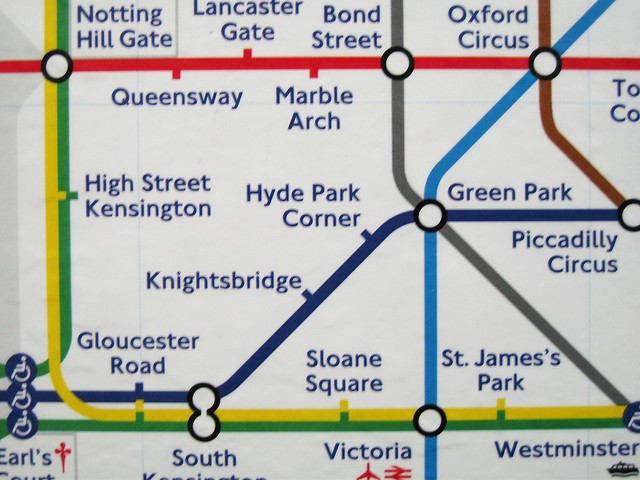
\includegraphics[scale=.50]{tubemap.jpg}
  \caption{\emph{London tube map}}
\end{subfigure}%
\begin{subfigure}{.5\textwidth}
  \centering
  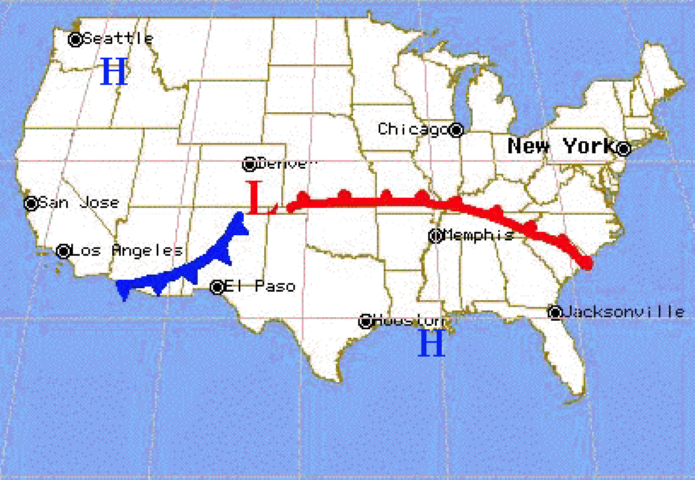
\includegraphics[scale=.25]{weather.png}
  \caption{\emph{Synoptic chart of weather in USA} }
\end{subfigure}
\begin{subfigure}{.5\textwidth}
  \centering
  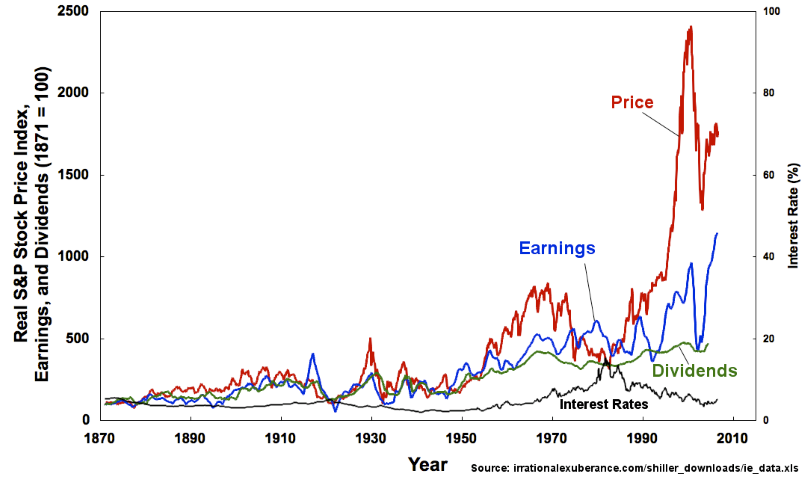
\includegraphics[scale=.25]{stockmarket.png}
  \caption{\emph{Plot of S\&P stock data} }
\end{subfigure}%
\begin{subfigure}{.5\textwidth}
  \centering
  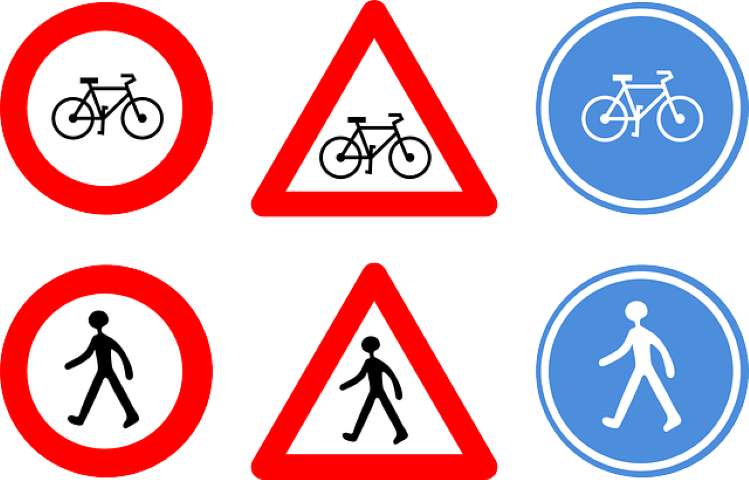
\includegraphics[scale=.25]{roadsigns.png}
  \caption{\emph{Bicycle and walking road signs} }
\end{subfigure}
\caption{\textit{Visualisation examples} (a)\citep{tubemap} (b)\citep{weather} (c)\citep{stockmarket}  (d)\citep{roadsigns}}
\label{fig:visualisations}
\end{figure}


\begin{figure}[!htb]
\centering

\begin{subfigure}{.5\textwidth}
  \centering
  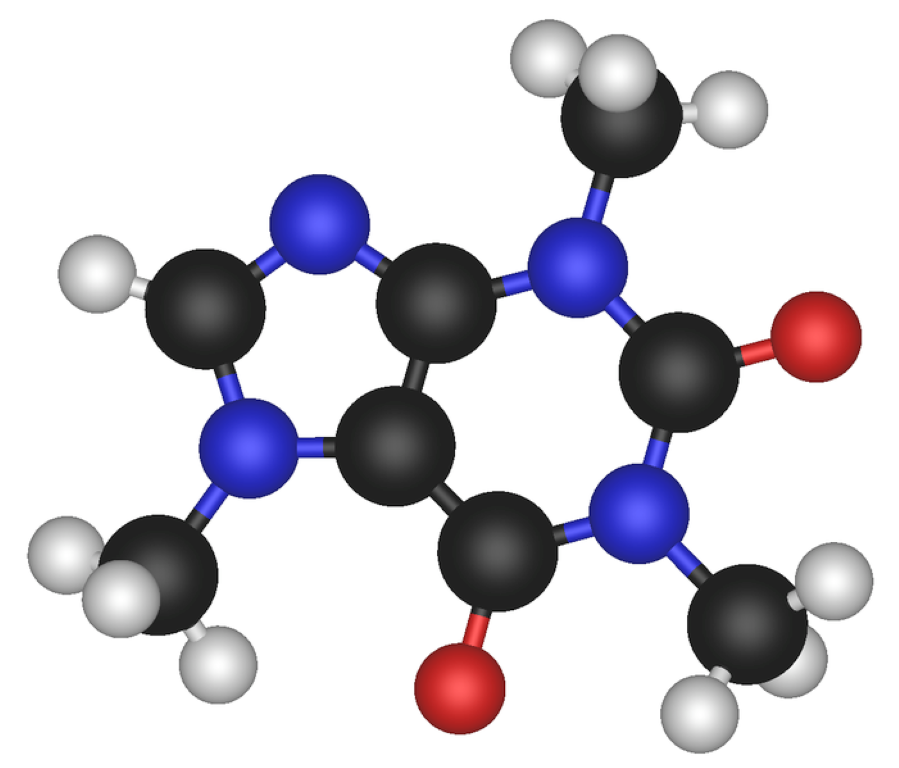
\includegraphics[scale=.20]{molecule.png}
  \caption{\emph{Caffeine molecule}}
\end{subfigure}%
\begin{subfigure}{.5\textwidth}
  \centering
  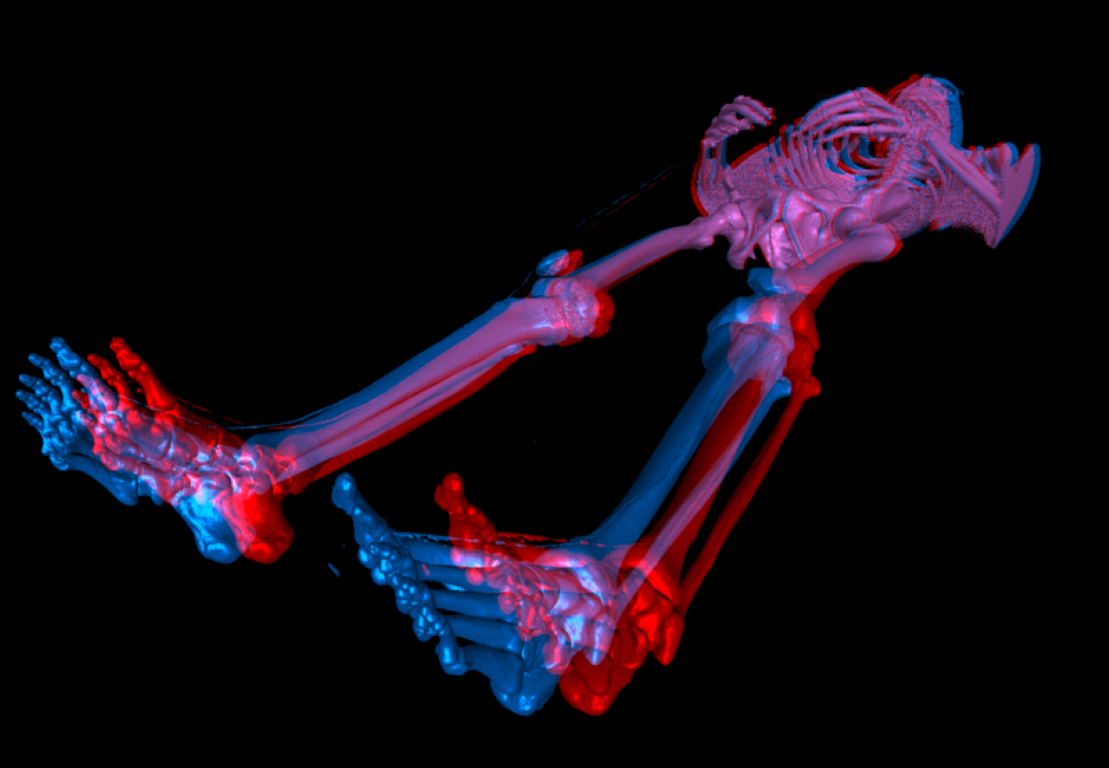
\includegraphics[scale=.20]{medicalvis.png}
  \caption{\emph{An anaglyph image of a human body} }
\end{subfigure}
\begin{subfigure}{.5\textwidth}
  \centering
  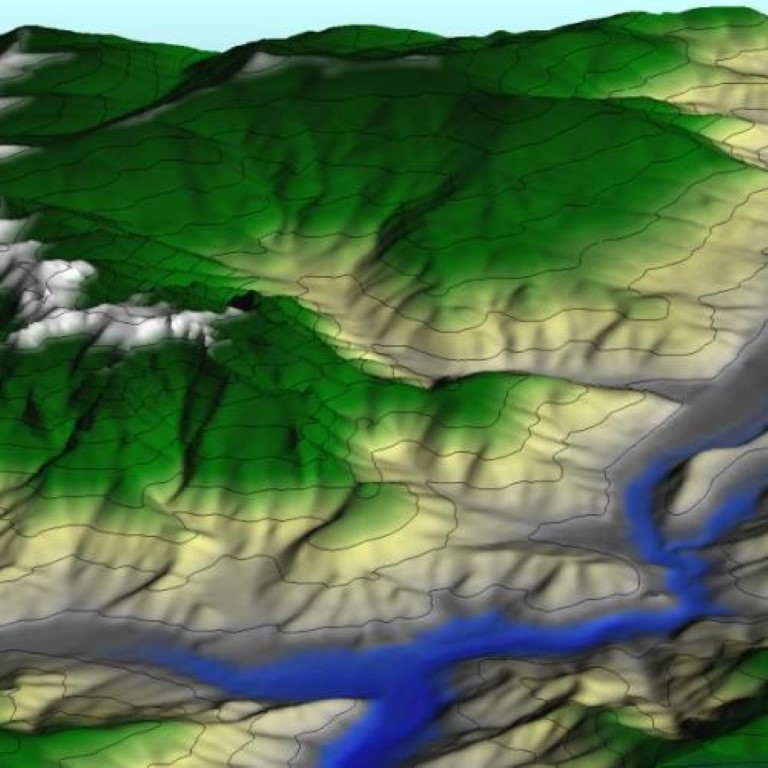
\includegraphics[scale=.20]{terrain.jpg}
  \caption{\emph{Terrain rendering} }
\end{subfigure}%
\begin{subfigure}{.5\textwidth}
  \centering
  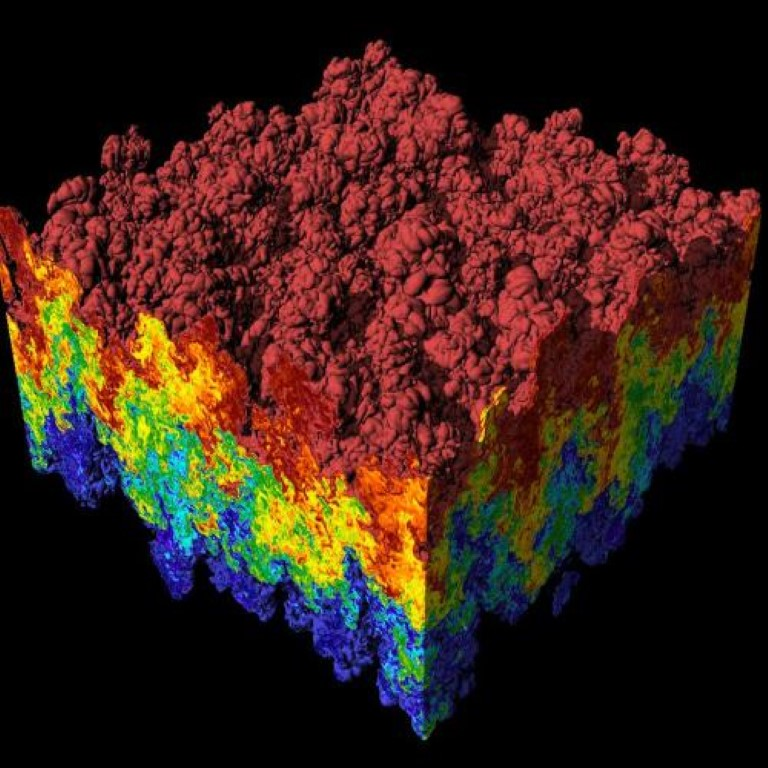
\includegraphics[scale=.20]{RayleighTaylor.jpg}
  \caption{\emph{Rayleigh-Taylor instability simulation} }
\end{subfigure}
\caption{\textit{Scientific visualisation} (a)\citep{molecule} (b)\citep{medicalvis} (c)\citep{rayleightaylor}  (d)\citep{terrain}}
\label{fig:scientificvisualisations}
\end{figure}

\subsection{Perception and cognition}

Cognition is a group of mental processes that includes attention, memory, learning, reasoning, and decision making. Perception is the processing of sensory information and is therefore a part of human cognition. Humans have a well developed sense of sight --- we perceive 75 percent of real world information visually. Visualisation is effective because it takes advantage of the brain's abilities, allowing us to gain insight more intuitively rather than through conscious thinking. 

\subsection{Visual search}

Visual search is a perceptual task requiring attention that involves the viewer actively scanning a visualisation or visual environment for a certain object or feature (the target) among other objects. There are various factors that can influence search performance. Basic attributes that can be considered to guide the deployment of attention (with a strong likelihood of supporting efficient search) are colour, motion, orientation and size \citep{wolfe04}.

\subsection{Graphical representation}

Visualisations are built from shapes and lines which have various properties such as size, length, width, height, volume, position, and colour. Additionally, these primitives can have dynamics that change over time, for example blinking or flashing. These visual properties are what is used to encode the information in a visualisation.

Visualisations can also consist of text (tag clouds introduced in \S\ref{sect:tagclouds} are an extreme example of this --- other visualisations may use text in passing, such as labelling an icon). Text can be manipulated to encode information through the use of typographical elements such as colour, font face and font styles.

\subsection{General techniques}

There are a great number of visualisation techniques that can be used. \cite{keim96} classified visualisation techniques according to their display mode:

\begin{enumerate}
\item \emph{Pixel-oriented techniques.} The arrangement of pixels, each dimension value mapped to a coloured pixel, grouped into adjacent areas. Pixel displays generally use one pixel per data value, so this technique can allow visualisation of large amounts of data depending on the display resolution. Appropriate arrangement of pixels can provide information on correlations and dependencies.

\item  \emph{Geometric projection techniques.} Geometrically transformed visualisations such as scatterplot matrices and parallel coordinates aim to show interesting properties of multi-dimensional datasets. In a parallel coordinate visualisation, dimensional spaces are mapped onto two display dimensions with axes that are parallel to each other. Each data element is depicted by connected line segments which intersect each of the axes (see Figure~\ref{fig:parallelcoordinates}). 

\begin{figure}[!htb]
  	 \centering
   	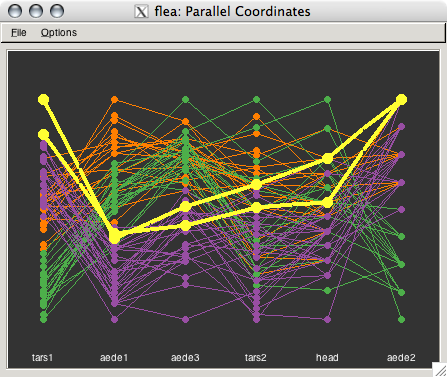
\includegraphics[scale=0.50]{parallelcoordinates.png}
  	\caption{\emph{Screenshot of GGobi, showing a parallel coordinate plot} \citep{parallelcoodinatesurl}}
	\label{fig:parallelcoordinates}
\end{figure}

\item  \emph{Icon-based techniques.} Iconic display methods map multi-dimensional data values to an icon by mapping the attribute values to features of the icon. An example of an iconic display is Chernoff faces \citep{chernoff73} as shown in Figure~\vref{fig:chernofffaces}. 

\begin{figure}[!htb]
  	 \centering
   	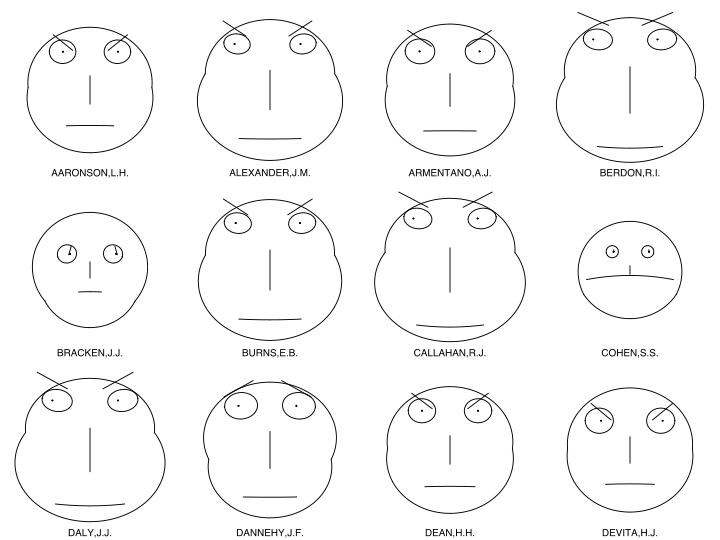
\includegraphics[scale=0.50]{chernofffaces.png}
  	\caption{\emph{Chernoff faces for evaluations of US judges} \citep{chernofffacesurl}}
	\label{fig:chernofffaces}
\end{figure}

\item  \emph{Hierarchical techniques.} Hierarchies are often drawn as node and edge diagrams, where a node is represented by a shape, and edges are represented by lines. Node and edge diagrams make inefficient use of space, with emptiness at the top left and right. Screen-filling techniques such as treemaps (see Figure~\vref{fig:treemap}) have been developed to fit large hierarchies onto the screen and use space more efficiently.

\item  \emph{Graph-based techniques.} Graph drawing facilitates understanding of relationships between objects. Graph-based techniques are used in trees, word graphs, and workflow diagrams. Specific layout algorithms are used to present large graphs.
\end{enumerate}

\subsection{Interaction techniques}

Interaction techniques are features that provide users with the ability to manipulate and interpret visualisations. There are a variety of ways that a user can interact and explore the data, for example:

\begin{description}
\item [Focus+Context] The underlying premise of Focus+Context is that the user may need both overview and detail information simultaneously. These two types of information can be combined within a single display, through interaction techniques such as fish-eye.

\item [Filtering] Uninteresting data elements can be filtered out. Dynamic queries can allow users to control the contents of the display, and focus on items of interest through elimination of other items.

\item [Zoom]  Items of interest may be zoomed in on. If users wish to know more about a particular area of the data, they can point to this location and click a mouse button until the required level of zooming is achieved.

\item [Brushing and linking] Brushing and linking allows multiple visualisations of a dataset to be be viewed simultaneously. Brushing of markers within the visualisations (such as in a scatterplot matrix) can then occur. The brushing and linking process involves selecting one element in a set of visualisations, brushing it with colour, then viewing the other linked visualisations to see the effect.

\end{description}

\section{Software visualisation}\label{sect:softvis}

As in information visualisation, in software engineering we want to explore abstract data to find trends and other interesting phenomena. We need help to comprehend and improve existing structures and build new ones. The examples given in Figures~\ref{fig:visualisations} and \ref{fig:scientificvisualisations} of information and scientific visualisation were all created with software. Given the success of visualisation in scientific and other research disciplines and the prolific examples of information visualisation and graphics in everyday life, computer generated visualisation and software engineering should be ideally suited. However, software visualisation is not widely practised or integrated into mainstream development environments.  An exception to this rule is UML diagrams, which are often used to create system diagrams of class structures and interactions (see Figure~\vref{fig:uml}). Even these diagrams, though, are often used for the development of new systems and may be largely ignored after the fact.

\begin{figure}[!htb]
   	\centering
  	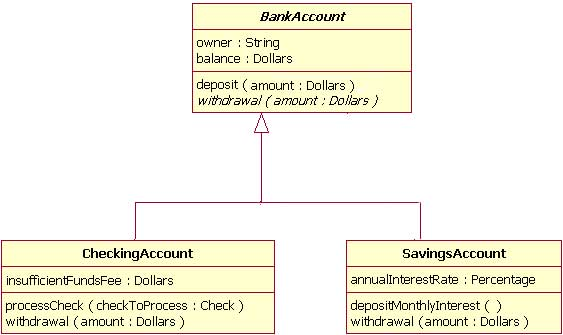
\includegraphics[scale=0.40]{uml.jpg}	
	\caption{\textit{UML Inheritance Diagram} \citep{uml}}
	\label{fig:uml}
\end{figure}

So what is the reason for the current lack of enthusiasm for software visualisation? \citet{reiss05} discusses this conundrum in his paper ``The paradox of Software Visualisation'', and outlines various possibilities which include reasons such as; lack of scaling to a suitable dataset size, interactive tools not providing answers to specific questions, low development workflow integration, lack of ease of use and high learning time, and neglect to adequately prove benefits. In the following sections, we describe the areas of software development where visualisations have been proposed, and introduce various devised techniques.

\subsection{What can we visualise?}\label{sect:whattovisualise}

Visualisation of software artefacts can help us in a number of areas, such as those detailed in Table~\vref{table:softwareartefacts}. A variety of approaches have been proposed for these areas.

\begin{table*}
\centering
\caption{\textit{Visualisation of Software Artefacts}}
\begin{tabular}{|p{6cm}|p{6cm}|} \hline
\textbf{Type}&\textbf{Area}\\ \hline
Quality assurance & metrics\par code smells\par heuristics \\ \hline
Process management & story/task management\par time allocation and management\par anomaly/issue detection\par project trends\par user achievement\par production support \\ \hline
Architecture & algorithms and control flow\par relationships and hierarchies\par interactions\par \\ \hline
Software evolution & source code repositories\par metrics\par structures \\ \hline
Runtime data & debugging\par memory management \\
\hline\end{tabular}
\label{table:softwareartefacts}
\end{table*}

\subsection{Quality assurance}\label{sect:qualityassurance}
 
Visualisation of software quality metric data often involves using a selection of multi-variate data visualisation techniques such as histograms, scatterplots or parallel coordinates. Kiviat charts (star glyphs) are also a commonly used technique for displaying multi-dimensional data.

Various 3D visualisations based on real-world metaphors like cities and landscapes have been developed. These have been applied in both software quality and architectural areas \citep[such as][]{irwin03, alam07} where metaphors such as 3D virtual worlds and building blocks have been explored.

It is possible to create ambient visualisations using alternate senses such as sound, odour, or vibration. \citet{murphyhill10} proposed a novel smell detector called Stench Blossom, that provided an interactive ambient visualisation designed to give programmers a high-level overview of the smells in their code. This and other visualisations of code smells such as jCosmo \citep{emden02} have been integrated in the development environment via a plugin.

\subsection{Process management}

Agile methodologies, used popularly in software project management, are inherently visual. Board views (used for story and task management) and burndown charts (time management, team status progression) are used in many agile teams. Also widely used are Gantt charts (a type of bar chart), which are visualisations incorporated into project management software illustrating a project schedule. 

\subsection{Architecture}

Algorithm visualisations for structured programming may be generated with graphical notations Nassi\textemdash Shneiderman diagrams (structograms). Nested boxes are used to represent simple statements and program control flow. Control flow graphs, first introduced by Frances E. Allen \citep{allen70}, show all paths that might be traversed through a program during its execution. These graphs are used in compiler optimisation and static program analysis tools.

Created by Booch, Rumbaugh and Jacobsen, Unified Modelling Language (UML) \citep{umlomg} is a popular and widely used set of graphical notations used to display relationships, interaction models and hierarchies in software. The set is comprised of a large number of diagrams including class/object models, use cases, behaviour and interaction diagrams, implementation diagrams and model management. These diagrams are most frequently used to visualise architectural elements of software.

Created by Ben Shneiderman in the nineties \citep{shneiderman09}, treemaps can show hierarchical data such as that found in software architecture, through the use of nested rectangles (see Figure~\vref{fig:treemap}).

\begin{figure} [!htb]
  	 \centering
   	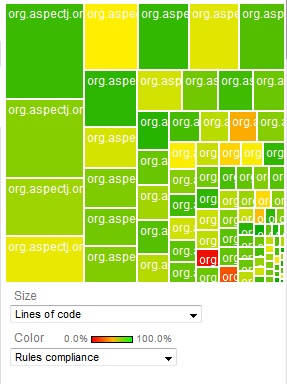
\includegraphics[width=60mm]{treemap.png}
  	\caption{\textit{Aspectj Treemap (created by the Sonar Software Analysis Platform)}}
	\label{fig:treemap}
\end{figure}

\subsection{Software evolution}

Visualisations of source code version histories are produced to analyse the evolution of a software system over time. This can reveal commonalities and irregularities in the development process. An example of this kind of visualisation is a `revision tower' \citep{taylor02} which allows people to see active areas of a project, how often changes are made, and how work is shared out.

Some tools produce visualisations of software metrics over time in order to provide a useful picture of software quality trends. One such example of this is the `SeeSoft system'\citep{eick92} which produces a space-filling visualisation for software metrics that are related to individual lines of code. Metrics such as code age can be viewed colour-coded, so that it is possible to see what parts of the system have recently been touched.

\subsection{Runtime data}

Dynamically generated visualisations to assist the debugging of runtime data are sometimes included as plugins in the development environment, such as the Eclipse Memory Analyser (MAT)\footnote{\url{http://www.eclipse.org/mat/}}. These tools may use a collection of visualisation techniques such as histograms, pie-charts and line graphs to illustrate measurements.

\section{Tag clouds}\label{sect:tagclouds}

Tag clouds are a common example of information visualisation found on the World Wide Web and are used to embody text --- words, two-word phrases and symbols. These items are grouped together to form a visual representation of the data.  Each element of the visualisation is referred to as a tag --- this may be website keywords which are hyperlinked to related resources. The frequency of a word (and therefore assumed importance) is highlighted by the font size or colour.  This makes the most important and prominent keywords easy to quickly identify as well as showing the relative importance of keywords. They can be displayed in a variety of layouts, most commonly alphabetically (see Figure~\vref{fig:tagcrowd} for a typical example).

\begin{figure}[htb]
   \centering
   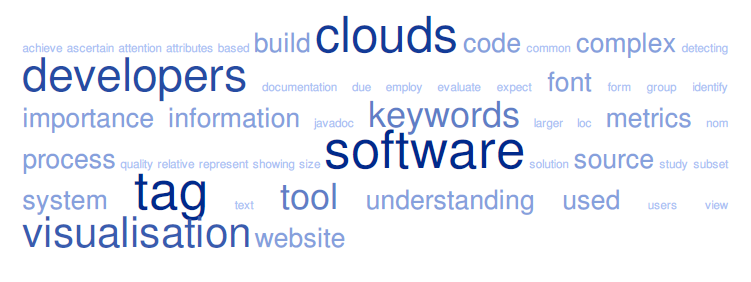
\includegraphics[width=140mm]{tagcrowd.png}
  \caption{\emph{Tag cloud created by TagCrowd}}
  \label{fig:tagcrowd}
\end{figure}

An early example of a weighted list of keywords can be found in Douglas Coupland's 1995 novel Microserfs. In this novel, a computer algorithm selects random phrases from an electronic diary creating a set of ``subconcious files''. In 2002 Jim Flanagan created a Perl module (Search Referral Zeitgeist), which generated a graphic of website referrers. Based on this implementation, photosharing site Flickr\footnote{\url{http://www.flickr.com}}, founded in 2004, created a ``tag cloud'' visualisation showing tag popularity through font size. Tag clouds then started appearing as a navigation aid on Web 2.0 websites such as Del.iocio.us\footnote{Now known as \url{http://www.delicious.com/}}.

The tag cloud was further adapted in 2006 by TagCrowd\footnote{\url{http://tagcrowd.com/}} for visualising word frequency in text, and then popularised by Wordle\footnote{\url{http://wordle.net/}} \citep{feinberg10}. Wordle showed tag clouds had the ability to be aesthetically pleasing (see Figure~\ref{fig:wordle}).

\begin{figure}[!htb]
   	\centering
   	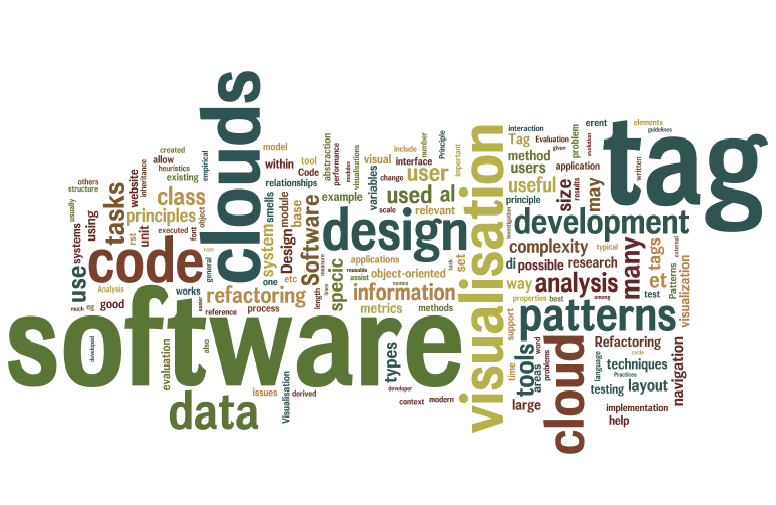
\includegraphics[width=140mm]{thesistagcloud.png}
  	\caption{\emph{Tag cloud created by Wordle}}
	\label{fig:wordle}	
\end{figure}

\subsection{Why tag clouds?}\label{sect:whytagclouds}

Tag clouds initially appear simple. This, along with high exposure online, makes them potentially more accessible to users than visualisations such as treemaps. This apparent simplicity may positively effect ease of use and learning ability, which were identified as important factors to visualisation takeup in the software engineering industry \citep{reiss05}. Another potential benefit of tag clouds is that they are reportedly perceived by some users to be visually interesting, appealing or otherwise aesthetically pleasing \citep{hearst08}. Some studies \citep[such as][]{kuo07} have also reported a high level of user satisfaction using them. 

In tag cloud visualisation, text labels are an intrinsic part of the visual encoding. This is particularly beneficial for software engineering datasets where textual labels are often used as identifiers.

Most current tag cloud implementations support limited interactivity. In order to effectively explore large datasets greater interactivity needs to be incorporated into the tag cloud visualisation interface, such as adding support for Shneiderman's visual information seeking mantra \citep{schneiderman96}.

\subsection{Tag clouds in software engineering}\label{sect:tagcloudsinsoftware}

In the software engineering domain, industry tools and academic research have not largely embraced tag clouds as a visualisation technique. There has been discussion of tag clouds for visualising relationships and structure \citep[such as][]{anslow08, bajracharya10, kurtz11} and also for source control evolution \citep[][]{kuhn12}. These examples show some interesting possibilities for inclusion of tag cloud based techniques in software engineering, but more extensive empirical evaluations are needed (of these papers only \citet{kurtz11} was included in the systematic mapping study detailed in Chapter~\ref{chap:strateval}, as it involved a usability evaluation). 

\subsection{Sourcecloud} 

In industry there are very few existing software engineering tools which utilise a tag cloud visualisation technique. Eclipse plugin Sourcecloud\footnote{\label{sourcecloud}\url{http://misto.ch/tag/eclipse/}} produces a Wordle-like visualisation of the text within a class, package or project with font size weighted by term frequency and colours assigned arbitrarily. The motivation behind this tool is to give an impression of how easy the code base is to understand by comparing proportions of domain-specific classname tags against core Java API classname tags.  We produced a visualisation of opensource project Aspectj\footnote{\label{aspectj}\url{http://www.eclipse.org/aspectj/}} (see Figure~\vref{fig:sourcecloud}). Some problems are apparent: the use of colour is a distracting factor (as it is not mapped to any variable), so some tags may appear more important than others without reason. An overview of all classes cannot be seen (due to a maximum word parameter), so words we are interested in may not be visible.

\begin{figure}[!htb]
   	\centering
  	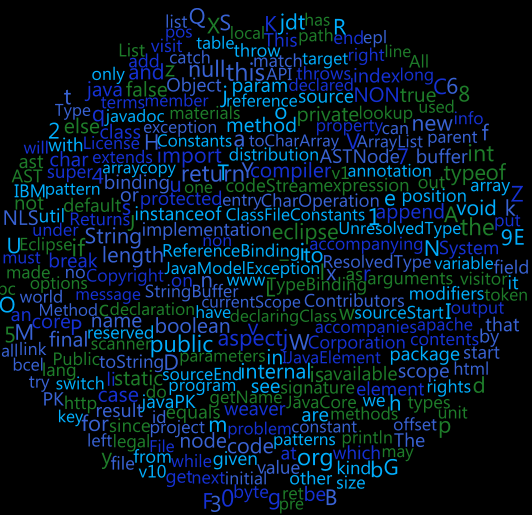
\includegraphics[scale=0.70]{sourcecloud.png}	
	\caption{\textit{AspectJ\textsuperscript{\ref{aspectj}} source code visualised with Sourcecloud\textsuperscript{\ref{sourcecloud}} }}
	\label{fig:sourcecloud}
\end{figure}

\subsection{Sonar platform} 

The Sonar Software Analysis Platform\footnote{\url{http://www.sonarsource.org/}}, which allows users to explore and visualise software metric data, comes bundled with a tag cloud component (see Figure~\vref{fig:aspectjsonar}). The tag font size is mapped to metric LOC (number of code lines for the class) and the tag colour is mapped to a rules compliance metric. The class name without the package can be problematic if different packages contained identically named classes. On the other hand, inclusion of the package name could dramatically increase the size of the cloud. The cloud produced is already a very large tag cloud, and may require scrolling. On the plus side, it is easy to quickly identify which classes contain a relatively large number of lines (CompletionEngine, CodeStream etc). The Sonar cloud tags are also used for navigation, and are hyperlinked through to pages showing individual metric data for the selected class. 

\begin{figure}[!htb]
   \centering
   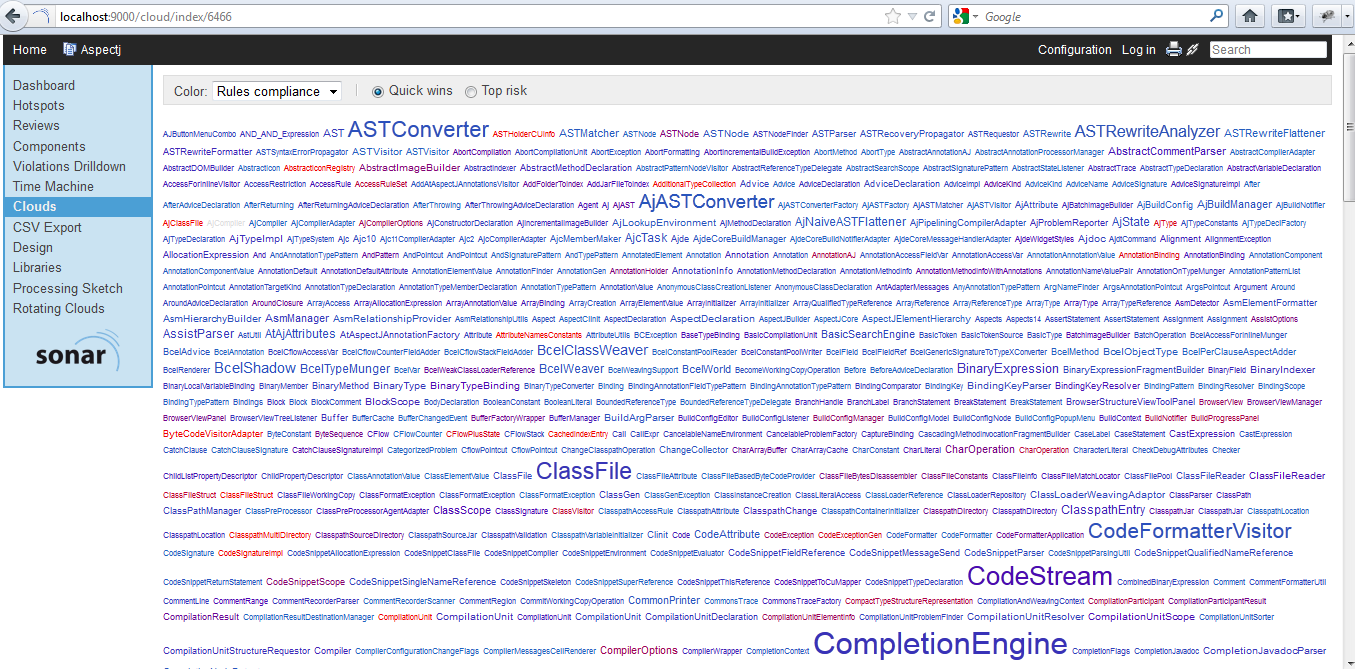
\includegraphics[scale=0.40]{sonarcloud.png}
  \caption{\textit{AspectJ\textsuperscript{\ref{aspectj}} visualised in Sonar}}
  \label{fig:aspectjsonar}
\end{figure}

\section{Summary and discussion} 

There is a comprehension problem in software development created by the huge size, constantly evolving nature and complex relationships. Modern ways to tackle aspects of scale and complexity include iterative development methodologies, automated unit testing and static or dynamic code analysis tools. Visualisation is a way to handle the reduced, but still overwhelming datasets we need to deal with in software engineering, and is considered useful in other domains (such as scientific research) as well as in general daily life. Despite a plethora of visualisation techniques suggested for the software domain, there remains a lack of widespread use of such techniques. 

Tag clouds are a highly recognisable visualisation of low-level complexity which deal primarily with text. Conventional implementations of tag clouds have limited interactivity which creates issues for data exploration. This research is focused on the evaluation of an interactive tag cloud visualisation tool. Can the tag cloud metaphor be extended to successfully visualise multi-variate data such as that found in software engineering? Both the Sourcecloud plugin and the Sonar platform visualisation show it is possible to apply the tag cloud technique directly to source code to identify and explore software quality metrics. Correspondingly, they also show the effectiveness of the technique relies on careful consideration given to various issues such as user perception of visual properties, and rich interactive features to allow data exploration.


% ------------------------------------------------------------------------


%%% Local Variables: 
%%% mode: latex
%%% TeX-master: "../thesis"
%%% End: 


%Software visualisation
% \include{Chapters/SoftwareVisualisation/softwarevisualisationquote}
%\include{Chapters/SoftwareVisualisation/softwarevisualisation}

%Exploring tag cloud design
% \include{Chapters/TagCloudDesign/tagclouddesignquote}
\chapter{Design Considerations for Interactive Tag Cloud Visualisation}
\label{chap:tagcloud}
\ifpdf
    \graphicspath{{Chapters/TagCloudDesign/TagCloudDesignFigs/PNG/}{Chapters/TagCloudDesign/TagCloudDesignFigs/PDF/}{Chapters/TagCloudDesign/TagCloudDesignFigs/}}
\else
    \graphicspath{{Chapters/TagCloudDesign/TagCloudDesignFigs/EPS/}{Chapters/TagCloudDesign/TagCloudDesignFigs/}}
\fi


Tag clouds have been used to visualise books, speeches, and other text through online tools such as Wordle\footnote{\url{http://wordle.net/}}, TagCrowd\footnote{\url{http://tagcrowd.com/}} and Manyeyes\footnote{\url{http://www-958.ibm.com/software/analytics/manyeyes/}}. While these tools easily create aesthetically pleasing clouds for users, their full potential for information visualisation is unrealised. As we saw in \S\ref{sect:tagcloudsinsoftware}, those few tools which have sought to apply the tag cloud paradigm to multi-variate data, have failed to take into consideration certain aspects (such as long identifiers) which have consequently proved problematic. In this chapter we develop design considerations for an interactive tag cloud visualisation system by reviewing design principles, guidelines, and research in general information and tag cloud visualisation. Furthermore, we present a set of task types that should be supported in order to enable data exploration. These task types are generated from analysing the challenges in visualising software and multi-variate data, as well as the capabilities of tag clouds. The task types and design considerations are used to inform the design of our interactive tag cloud visualisation system `Taggle', presented in Chapter~\ref{chap:taggle}.

\section{Visual variables}\label{sect:visualvariables}

Tools such as Wordle or TagCrowd generate tag clouds which display word frequency counts through the font size of individual tags. Other visual properties (such as colour, ordering and typeface styles) are generally ignored or used in a decorative fashion. We contend that these alternate visual properties available in tag clouds can and should be used to represent other data variables or reinforce mappings. With these visual properties representing data, a tag cloud can support users in tasks such as gisting, searching and knowledge extraction. In the creation of our interactive tag cloud visualisation system Taggle, consideration had to be given to the amount of influence on user perception for each visual variable, as well as their individual properties which affected suitability of being mapped to data. 

Due to the textual nature of tag cloud visualisation, many visual properties in tag clouds relate to font characteristics. Phrase or keyword emphasis in tag clouds are manipulated via typographical techniques. These can be applied with various design principles \citep[such as those outlined in the seminal manual ``The elements of typographical style''][]{bringhurst01}. Tag emphasis in clouds (for individual data points) may be created through manipulation of variables such as size, colour, font family or style. Visual properties of tag clouds that may influence perception can be seen in Table~\vref{table:visualproperties}, although not all properties may be suitable to map to data variables. An example of data mapped to some of these properties may be seen in Figure~\vref{fig:tagmapping}.

\begin{table*}
\centering
\caption{\textit{Visual properties that may influence perception in tag clouds}}
\begin{tabular}{|p{4cm}|p{8cm}|} \hline
\textbf{Visual Property}&\textbf{Types}\\ \hline
Layout & typewriter\par spiral\\ \hline
Order & alphabetical\par semantic\par random\\ \hline
Tag length & variable number of characters\par equal number of characters\\ \hline
Tag position & top left quadrant\par top right quadrant\par bottom left quadrant\par bottom right quadrant\\ \hline
Font size & \\ \hline
Font family& Serif vs Sans-serif\par Arial\par Times New Roman \\ \hline
Font colour & hue\par saturation\par value \\ \hline
Background colour & hue\par saturation\par value \\ \hline
Font style & bold vs normal\par italics vs normal\par all capitals vs mixed case\par underline vs normal   \\ 
\hline\end{tabular}
\label{table:visualproperties}
\end{table*}

\begin{figure}[!htb]
	\centering
	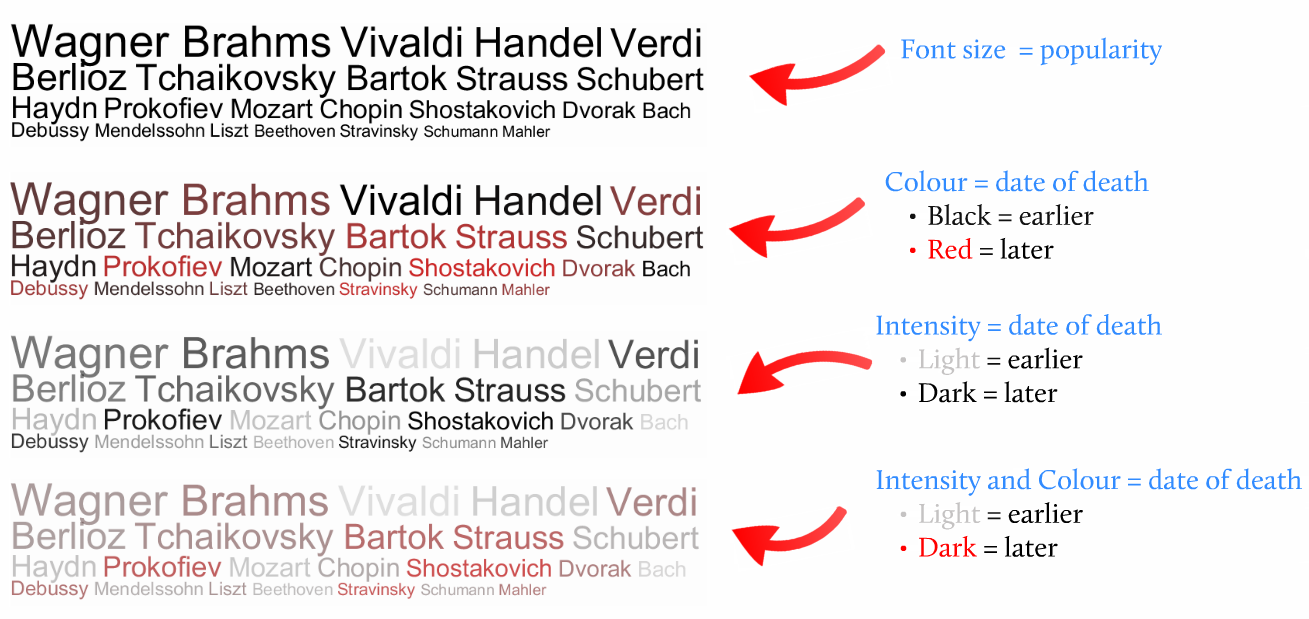
\includegraphics[scale=0.40]{mapping.png}
	\caption{\textit{Popularity ranking of composers: mapping of artificial data to tag cloud visual properties (tag clouds generated by Taggle).}}
	\label{fig:tagmapping}
\end{figure}

\subsection{Visual mapping} 

The term `visual variables', as introduced by \citet{bertin83} in the ``Semiology of Graphics'', refers to a specified set of symbols that can be applied to data in order to translate information. This process of mapping data to visual properties is called `visual mapping'. The visual variables are defined as position, size, shape, value, colour (hue), orientation, and texture. Choosing a particular variable to map to data depends on an analysis of the characteristics of the variable. Each variable's characteristics are defined from the following list of perceptual approaches:

\begin{itemize}
	\item Selective: If a data point can easily be selected as being different from the other data points.
	\item Associative: If multiple data points can be perceived as being similar.
 	\item Quantitative: If data points can be perceived as being proportional to one another.
 	\item Ordered: If data points can be interpreted in an order.
	%\item Length: How many values a variable can meaningfully contain.
\end{itemize}

When creating a data visualisation, it is important to know and appropriately use the characteristics of a visual variable. In the following subsections the effects on user perception for each tag cloud visual variable is discussed with respect to Bertin's perceptual approaches, other design guidelines and tag cloud research. Likely suitability for data mapping within a tag cloud is determined.

\subsection{Layout and order}\label{sub:layout}

Layouts of tags within a tag cloud are generally based on either a typewriter style (tags arranged from left to right, and top to bottom), or arranged in a spiral pattern. Relevant ordering of the tags within the tag cloud layout (within constraints imposed by such things as window shape) is important for users of the visualisation tools when applying search and locate tasks. Previous research has indicated alphabetical ordering of tags is generally preferable to random or semantically clustered layouts when searching for a named tag within a tag cloud, although semantic clustering can provide improvements over random arrangements \citep[][]{halvey07, schrammel09}. 

However, the ordering property is also suitable for search and locate tasks using variables not related to the tag text. For instance, using the ordering property to locate tags with maximum or minimum values of a variable, in Figure~\vref{fig:datasets1} once it is understood that the ordering of the tags is related to the popularity of a name within the USA, it is easily found that the top three most popular boys names in the US are Michael, Christopher and Matthew. Likewise, in Figure~\vref{fig:background}, it can easily be seen that Bahamas had the greatest number of gold medals in the Olympic medal ranking based on a per-capita ranking system.

\begin{itemize}
	\item \emph{\textbf{Tag order:} Visual property tag order is suitable for mapping to data fields}
\end{itemize}

\subsection{Tag length and position} 

Longer tag lengths have been shown to have an effect on user perception of tag importance \citep{bateman08}. Tags placed in the upper left quadrant of a tag cloud are found more quickly \citep{bateman08} and are also better recalled \citep{rivadeneira07}. Analysis of eye-tracking data has shown the upper left quadrant of a tag cloud receives the most attention \citep[][]{lohmann09, schrammel09b}. It is possible the upper left quadrant dominance is due to western language reading patterns. Due to this quadrant prominence, tag position is a particularly appropriate mapping for search and locate tasks through use of the ordering property (\S\ref{sub:layout}) when tag clouds are arranged in a typewriter fashion. 

\begin{itemize}
	\item \emph{\textbf{Equal length tag identifiers:} It should be possible to set the length of the tag identifiers to an equal length to minimise effects on user perception}
\end{itemize}

\subsection{Font size} \label{sect:fontsize}

Text size manipulation can be a very effective way of creating emphasis. Empirical research on tag cloud visual properties has identified size as having a significant effect on user perception \citep[for example][]{lohmann09, bateman08, halvey07}. This means large font sized tags are found more quickly than small font sized tags. For example, in Figure~\vref{fig:datasets2} user names `pam120', `kfc172' or `gey66' can immediately be located in the tag cloud due to their prominence from a comparatively large font size.

The size visual variable is selective, associative, ordered, and quantitative \citep{bertin83}, although care must be taken when using size quantitatively, as changes in size from volume or area may be difficult to interpret \citep{carpendale03}. According to \citep{bateman08, schrammel09b} font size can be accurately compared in a tag cloud.

Because of canvas and screen boundaries, there are limitations in the maximum font sizes which can be displayed within a tag cloud. With regard to minimum font sizes, guidelines based on reading performance research state a 9pt font limit for web pages or screen media \citep[pg 107, chap 11:8][]{usability06}.
 
For data mapping purposes, font size is an appropriate visual variable candidate for mapping to data variables in a tag cloud. Careful attention should be paid to minimum font sizes for reading ease. 

\begin{itemize}
	\item \emph{\textbf{Font size:} Visual property tag order is suitable for mapping to data fields}	
	\item \emph{\textbf{Constrained font sizes:} Font size should be constrained to greater than 9pt, and a suitable maximum font size according to canvas and screen boundaries}
	\item \emph{\textbf{Comparable tags:} Tags should be able to be compared by moving closer together to assist quantitative comparisons}
\end{itemize}

\subsection{Font Family}   

Typographical characteristics such as font family were not mentioned by \citet{bertin83}. The shape visual variable, which is the most closely related variable mentioned, is not perceived as an especially effective variable. According to \citet{carpendale03}, shape may be selective and associative, providing there are minimal data points or minimal shape variations. 

In tag cloud research, \citet{waldner13} found text orientation and shape modifications performed significantly worse than colour coding for distinguishing tag categories. Many users also perceived rotated tags as unstructured and unattractive. Shape differences caused by serifs or font styles were hard to detect in controlled experiments using the Helvetica font style. It is also possible that manipulation of font family may alter user perception of other font styles used as a mapping variable, such as bold or italic. It does not seem that font family would be an effective data mapping visual property within a tag cloud. 

Research shows that reading speed is best when users are presented with familiar fonts such as Times New Roman, Arial or Helvetica  \citep[pg 106, chap 11:7][]{usability06}. These fonts may therefore be preferable in a tag cloud for reading accuracy.

\begin{itemize}
	\item \emph{\textbf{Font family:} Visual property tag order is not suitable for mapping to data fields}	
	\item \emph{\textbf{Familiar fonts:} For reading accuracy, fonts should be familiar such as Times New Roman, Arial or Helvetica}	
\end{itemize}

\subsection{Font colour}\label{sect:fontcolour}

In a study of the effectiveness of textual retinal properties in tag clouds, \citet{waldner13} found that after font size, colour (both as text colour or as the tag's background colour) was the most effective visual text variable for encoding nominal and ordinal data. On the other hand, transparency was disliked by users and lead to inaccurate results when determining tags of relevance. \citet{bateman08} found that colour intensity (saturation/transparency) had a relatively good influence on user perception, although not as strong as font size. 

\citet{preston10} investigated the effectiveness of typographical emphasis techniques (such as colour, bold and italics) on computer presentation software. They found that use of colour in font emphasis techniques generally elicited significantly faster response times identifying  text than achromatic techniques such as bold and italic, provided a suitable colour contrast was given.

Colour value has properties selective, associative and ordering \citep{bertin83}, whereas colour hue has only selective and associative properties and cannot be perceived by a viewer in an ordered fashion. Value may be considered to be quantitative also, in that lighter value colours are perceived to be related to smaller numbers and darker colour values to higher numbers, but actual quantitative comparison can be difficult (for example perceiving one shade of colour as being three times darker than another shade). 

Ware's information visualisation guidelines advise not using more than ten colours for coding symbols (especially if the symbols are to be used against a variety of backgrounds) \citep[pg 124, chap 4, G4.15][]{ware04}. Ware also recommends twelve specific colours for use in coding: red, green, yellow, black, blue, white, pink, cyan, grey, orange, brown, and purple \citep[pg 126, chap 4, G4.18][]{ware04}.

For data mapping purposes, it may be more useful to consider colour value and saturation as being aligned to a transparency mapping often employed as a visual property in tag clouds. Both hue and transparency are appropriate candidates for mapping to data variables in a tag cloud. Consideration must be given to colour choice, contrasts and quantitative mapping.

\begin{itemize}
	\item \emph{\textbf{Colour hue:} Visual property colour hue is suitable for mapping to data fields}	
	\item \emph{\textbf{Colour transparency:} Visual property colour transparency is suitable for mapping to data fields}	
	\item \emph{\textbf{Colour selection:} Colour codes should be taken from Ware's  colour code recommendations (red, green, yellow, black, blue, white, pink, cyan, grey, orange, brown, and purple)}	
\end{itemize}

\subsection{Background Colour}\label{sect:backgroundcolour}

Background colour is an appropriate data mapping visual variable as an alternative to font colour. As discussed in \S\ref{sect:fontcolour}, \citet{preston10} found that use of colour in typographical emphasis techniques elicited faster response times identifying emphasised text than achromatic techniques. This performance improvement was providing a suitable colour contrast was given (such as red, green or blue on a white background). Consideration of text colour against background must be given during colour selection of visual mappings within a tag cloud. 

It is possible to manipulate background colour on an individual tag. This could have two possible benefits 1) it allows grouping together of multiple keywords or phrases, and 2) mapping the colour to the background behind the tag may have a greater effect on user perception than mapping the colour to the text. This is because the area of the background behind the tag is greater than the area of the font text itself and in general, the larger the area that is colour coded, the more easily colours can be distinguished \citep[pg 125, chap 4][]{ware04}. Colour coding in the tag background has been found to support more accurate estimation of relevant tags than font colour \citep{waldner13}.

Chapter~\ref{chap:eval} details empirical research conducted which included investigation of the benefits of background colour manipulation in tag clouds. For an example of text and background colour in a tag cloud see Figure~\vref{fig:background}, which shows Olympic medal rankings using both gold first and per-capita ranking systems. Countries which have more than one word in their name are more easily distinguished using background colour mapping.

\begin{figure}[!htb]
\begin{subfigure}{\textwidth}
	\centering
	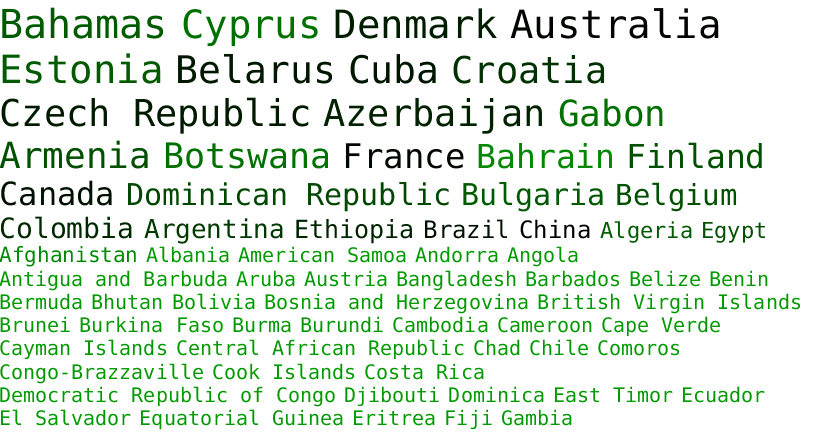
\includegraphics[scale=0.50]{foregroundex.png}
	\label{fig:foregroundsub}
	\caption{\textit{Font colour}}
\end{subfigure}
\begin{subfigure}{\textwidth}
  \centering
  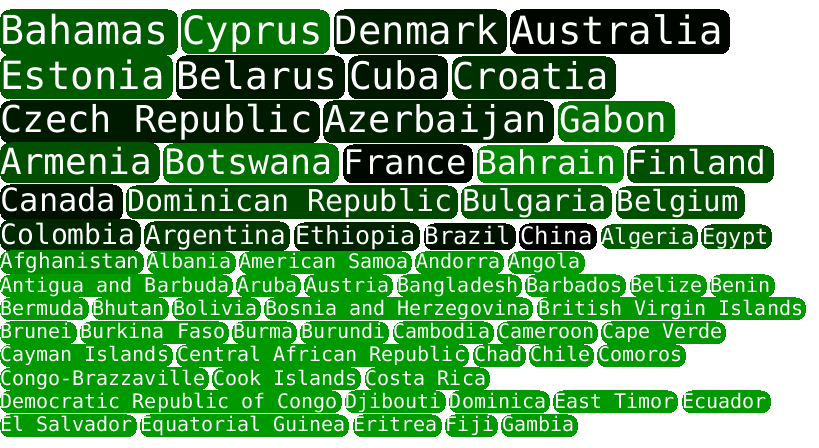
\includegraphics[scale=0.50]{backgroundex.png}
  \label{fig:backgroundsub}
  \caption{\textit{Background colour}}
\end{subfigure}
  \caption{\textit{Olympic medal rankings: size and order are mapped to per-capita ranking system. Colour is mapped to standard (gold first) ranking system.}}
  \label{fig:background}
\end{figure}

\begin{itemize}
	\item \emph{\textbf{Colour background:} Visual property colour background is suitable for mapping to data fields}	
	\item \emph{\textbf{Colour contrasts:} Strongly contrasting colour schemes should be selected such as red, green or blue on a white background}	
\end{itemize}

\subsection{Font Style}   

Font styles or typography in general were not included in Bertin's visual variables \citet{bertin83}. \citet{bateman08}'s exploration of the effects of various properties and characteristics of text in tag clouds found that weight (bold style) had a consistently strong influence on user perception. A comprehensive study on the effectiveness of emphasis techniques in presentations by \citet{preston10} found bold text performed well with black text on a white background but not with white text on black.  \citet{preston10} found capitals to be the most effective of the achromatic emphasis techniques, although all four techniques (capitals, bold, italics and underline) did not perform as well as the chromatic techniques (use of colour).  Underline and italic emphasis techniques were consistently the least effective means of emphasising text. 

Font styles bold and underline are considered more effective as text emphasis than italic or underline. The number of differing values that these typographical styles may show is only two (underline on, underline off --- bold on, bold off) so is likely not worth including as a data mapping variable in a tag cloud. 

\begin{itemize}
	\item \emph{\textbf{Font styles:} Visual property font styles are not considered suitable for mapping to data fields}	
\end{itemize}

\section{Challenges in software visualisation}\label{sect:challenges}

In the software engineering domain, quality metric data distributions are typically heavily skewed and may contain outliers (see Figure~\vref{fig:distributions}). Unlike some other disciplines, where outlying data points may be discarded or ignored, in software engineering these outliers are potentially the most interesting and should be investigated further as potential candidates for refactoring. 

\begin{figure}[!htb]
   	\centering
  	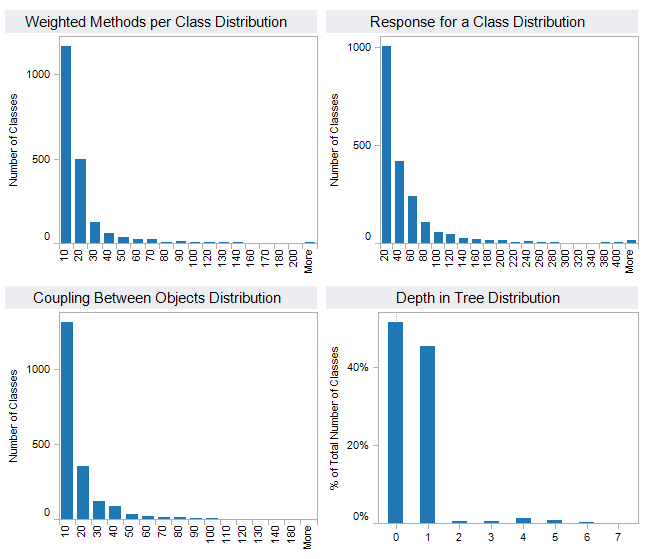
\includegraphics[scale=0.70]{distributions.png}	
	\caption{\textit{Distribution of Chidamber and Kemerer metrics for open source project AspectJ (calculated by CKJM toolkit)}}
	\label{fig:distributions}
\end{figure}

In the software visualisation domain, and many datasets in general, there may be a large numbers of data points which cover large ranges of values. There are also various size constraints to be considered such as the size of the screen, symbols, fonts or other identifiers. One general information visualisation technique for management of this problem is to incorporate interactivity into the visualisation, first providing the user with an overview, then zooming and filtering, and obtaining the information details on demand. This principle is called the ``Information Seeking Mantra'' and was introduced by \citet{schneiderman96}. Another technique is to display an overview of data but allow detailed information to be displayed simultaneously (also known as focus+context) such as with fish-eye. 

There is a variety of textual information contained in many general datasets, and software datasets are no exception (for example class, method or package names, bug categories and rankings, and agile stories and tasks). Text is problematic for some multi-variate visualisation techniques (such as scatterplots or treemaps) due to space limitations. No one visualisation method or technique may provide a good balance for all considerations for a software engineering dataset and a combination of techniques may be necessary, using whichever method is most effective for a particular context.

\section{Datasets for the tag cloud technique}\label{sect:datasets}

One of the benefits of tag cloud visualisation is that data point textual identifiers (such as names) are an integral part of the graphic, meaning that users don't have to navigate into the visualisation to find important information. With this in mind, the sort of dataset that would be optimal to display in a tag cloud is one which includes modest amounts of textual information. Many datasets include this sort of information, in the form of names, labels or identifiers. In a general capacity, example datasets that might be used include names of people, brand names or marketing data, company financial information, stock market or foreign exchanges, country statistics, animal endangerment ratings, sporting events, file and folder names in a computer, and so on. Software engineering datasets also contain this sort of data such as class, method or package names, bug categories and rankings, and agile stories and tasks. See Figures~\ref{fig:datasets1} and \ref{fig:datasets2} for examples of a general and software related dataset.

\begin{figure}[!htb]
	\centering
	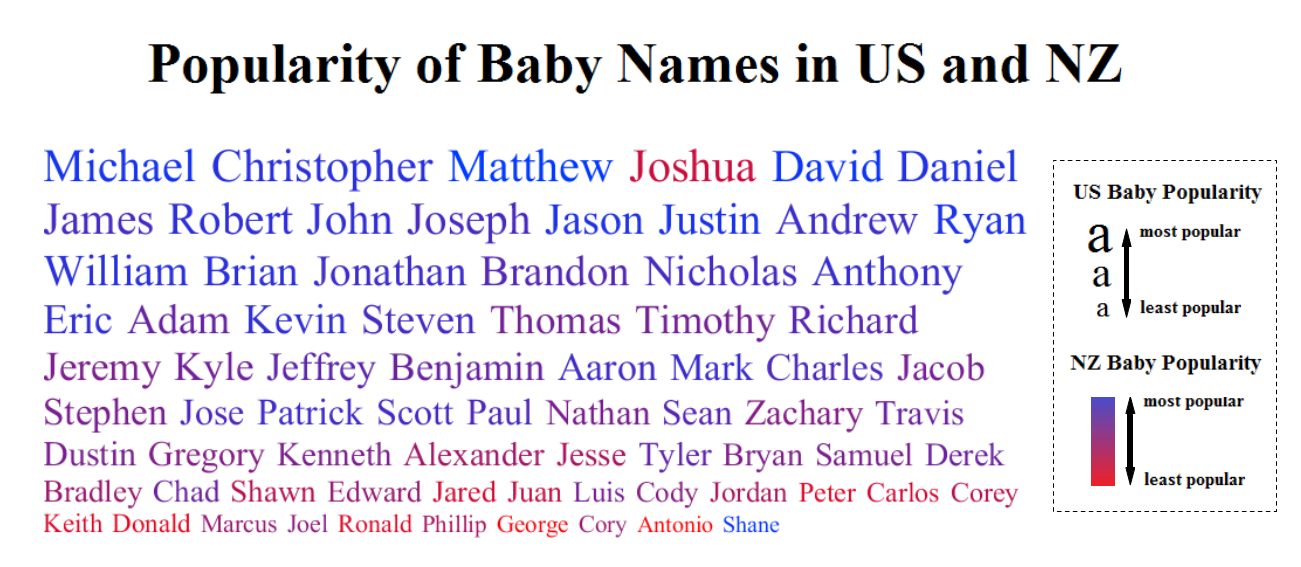
\includegraphics[scale=0.35]{babynames.png}
	\label{fig:babynames}
	\caption{\emph{Popularity of baby names}}
      \label{fig:datasets1}
\end{figure}

\begin{figure}[!htb]
  \centering
  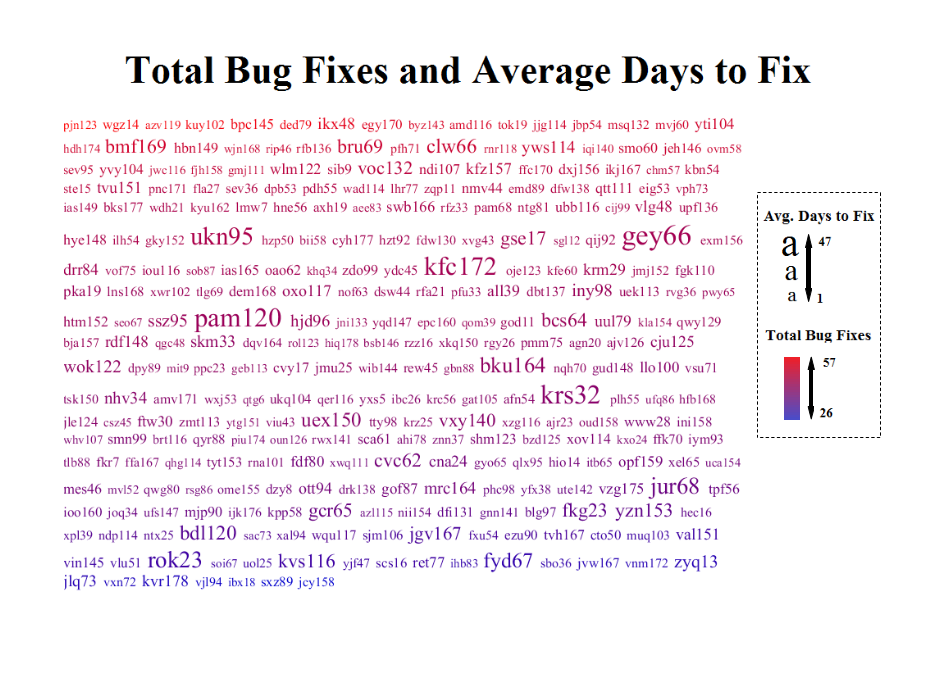
\includegraphics[scale=0.50]{buglist.png}
  \label{fig:buglist}
  \caption{\emph{Bug fixes for each user}}
  \label{fig:datasets2}
\end{figure}

Much of the important textual data contained in these sorts of datasets is a phrase or collection of words rather than just one word. Also, many datasets containing some sort of label or identifier utilise many characters --- such as a fully qualified file or class name. It is important to note that multiple word phrases and lengthy label names can waste valuable real estate in the visualisation. There are two possible issues with this 1) it may have the effect of the data point appearing to have more importance than it actually does due to the increased prominence of the text, and 2) with multiple word tags it may be difficult to distinguish the boundaries between data points (this can be seen in Figure~\vref{fig:birds}).

\begin{figure}[!htb]
	\centering
	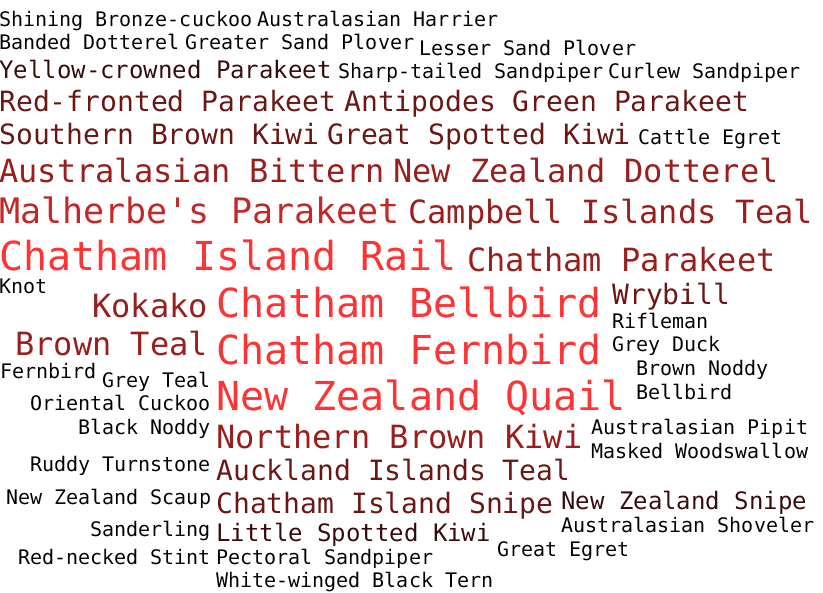
\includegraphics[scale=0.50]{birds.png}
	\caption{\emph{Endangered species ranking for NZ birds}}
	\label{fig:birds}
\end{figure}

\begin{itemize}
	\item \emph{\textbf{Textual datasets:} Optimal datasets contain textual identifiers such as class names or stories}
	\item \emph{\textbf{Filterable tag phrases:} Multiple words waste valuable real estate in a visualisation, so should be filterable}
	\item \emph{\textbf{Establish tag boundaries:} Boundaries between tags with multiple words should be clearly established}
\end{itemize}

\section{Task types to enable data exploration in a tag cloud}\label{sect:tasktypes}

It was suggested by \citet{rivadeneira07} in early empirical work, that the task set supported by tag clouds includes searching, browsing, impression forming and recognition/matching. Evidence exists that suggests tag clouds can provide improvements for summarising descriptive information (overviews) and also that they may be useful as a descriptive supplement for traditional search interfaces \citep{kuo07, sinclair08}. However, research has compared tag clouds negatively to tables or lists for search and locate tasks \citep[such as][]{oosterman10, halvey07, kuo07, rivadeneira07}. These experiments which report sub-optimal results for tag clouds required searching for or locating textual tag names and do not ask users to complete a visual search using additional features such as colour. (See Chapters~\ref{chap:exp1} and  \ref{chap:exp2} which investigate the possibility of the use of tag background colour or dual visual feature mapping improving user performance in a visual search.) Furthermore, we believe that more complex datasets (such as those with multiple data variables and intricate relationships between records) and other domain-specific factors, add more substance than the simplistic search and locate experiments might suggest. 

We have identified an appropriate set of tasks shown in Table~\vref{tab:taskset} which match the potential capabilities of tag clouds to tasks that are useful in software engineering (and also have a wider application in multi-variate data analysis). For categorisation purposes these can be further assigned to task types associated with data mining.

\begin{table}
\centering
\caption{\textit{Tasks}}
\begin{tabular}{|p{8cm}|p{3cm}|} \hline
 \textbf{Task Description} & \textbf{Task Type} \\ \hline
Identify similar characteristics of data & Clustering \\
Identify data distribution & Summarising \\
Identify data correlations & Associative \\
Detect outliers in a correlation & Summarising \\
Finding minimum/maximum values & Classifying \\
Comparison of data elements  & Classifying\\\hline
\end{tabular}
\label{tab:taskset}
\end{table}

As an example of how tag clouds may be used to complete the associative task of identify correlations between variable, see Figure~\vref{fig:tagcorrelation} which shows (artificially composited) composer popularity against the date of death. We can see that modern composers (who died later) are more popular than composers who died earlier such as those from the Classical or Baroque period. In Figure~\vref{fig:datasets2} we can use the tag cloud font size to establish a general data distribution (summarising task). Most user names in the tag cloud are very small with only a few larger names, therefore we can hypothesise that most users take a comparatively lower number of days to complete bug fixes.

\begin{figure}[!htb]
	\centering
	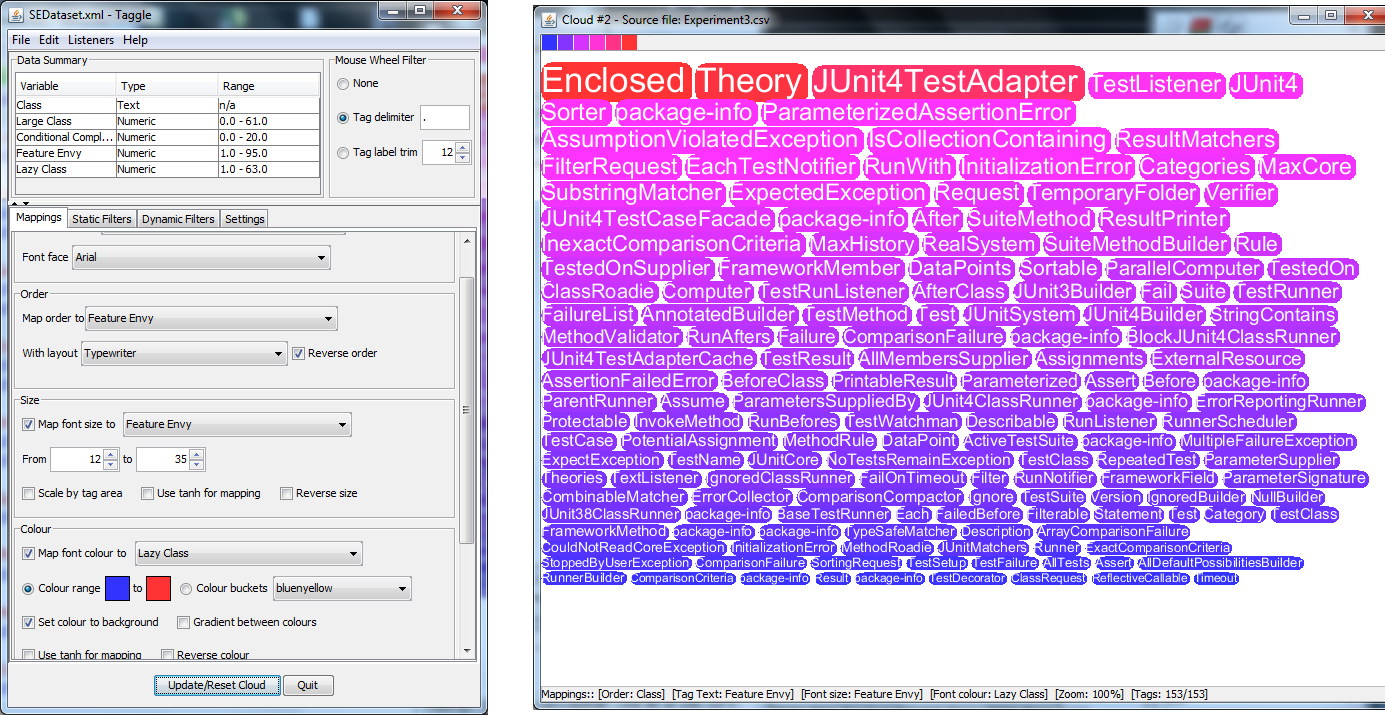
\includegraphics[scale=0.45]{correlation.png}
	\caption{\emph{Popularity ranking and composer date of death}}
	\label{fig:tagcorrelation}
\end{figure}

\section{Summary and discussion}

The design considerations for an interactive tag cloud visualisation tool presented in this chapter have been developed through analysis of current tag cloud and information visualisation research, guidelines, and principles. We summarise these considerations in Table~\ref{tab:designconsiderations}.

\begin{longtable}{|p{5cm}|p{9cm}|} 
%\caption{\textit{Design considerations for an interactive tag cloud tool}}
\hline
\textbf{Design Considerations} & \textbf{Description} \\
\hline
\endfirsthead
\multicolumn{2}{c}%
{\tablename\ \thetable\ -- \textit{Continued from previous page}} \\
\hline
\textbf{Design Considerations} & \textbf{Description} \\
\hline
\endhead
%\hline 

\multicolumn{2}{r}{\textit{Continued on next page}} \\
\endfoot
\hline
\endlastfoot
Textual datasets & Optimal datasets contain textual identifiers such as class names or stories.\\
Filterable tag phrases & Multiple words waste valuable real estate in a visualisation, so should be filterable.\\
Establish tag boundaries & Boundaries between tags with multiple words should be clearly established.\\
Tag order & Visual property tag order is suitable for mapping to data fields.\\
Equal length tag identifiers & It should be possible to set the length of the tag identifiers to an equal length to minimise effects on user perception.\\
Font size & Visual property tag order is suitable for mapping to data fields.\\	
Constrained font sizes & Font size should be constrained to greater than 9pt, and a suitable maximum font size according to canvas and screen boundaries.\\
Comparable tags & Tags should be able to be compared by moving closer together to assist quantitative comparisons.\\
Font family & Visual property tag order is not suitable for mapping to data fields.\\	
Familiar fonts & For reading accuracy, fonts should be familiar such as Times New Roman, Arial or Helvetica.\\	
Colour hue & Visual property colour hue is suitable for mapping to data fields.\\	
Colour transparency & Visual property colour transparency is suitable for mapping to data fields.\\	
Colour selection & Colour codes should be taken from Ware's  colour code recommendations (red, green, yellow, black, blue, white, pink, cyan, grey, orange, brown, and purple).\\	
Colour background & Visual property colour background is suitable for mapping to data fields.\\	
Colour contrasts & Strongly contrasting colour schemes should be selected such as red, blue and green on a white background.\\	
Font styles & Visual property font styles are not considered suitable for mapping to data fields.
\label{tab:designconsiderations}
\end{longtable}


In \S\ref{sect:tasktypes}, we presented a set of task types that we believe should be supported in a tag cloud visualisation tool in order to enable exploration of a software engineering dataset. These task types were generated from analysing software visualisation challenges and tag cloud capabilities. The task types and design considerations were used to inform the design of our interactive tag cloud visualisation system `Taggle', presented in Chapter~\ref{chap:taggle}.
	
% ------------------------------------------------------------------------


%%% Local Variables: 
%%% mode: latex
%%% TeX-master: "../thesis"
%%% End: 


%Introducing Taggle prototype
% %% Quotation for introducing the taggle prototype

\begin{savequote}[55mm]                                              
\sffamily Never try to solve all the problems at once - make them line up for you one-by-one. 
\qauthor{\textbf{Richard Sloma}}                        
\end{savequote}  

%%%-----------------------------
\chapter[Taggle: A Tag Cloud Visualisation Tool]{Taggle: A Tag Cloud Visualisation Tool}


\label{chap:taggle}
\ifpdf
    \graphicspath{{Chapters/Taggle/TaggleFigs/PNG/}{Chapters/Taggle/TaggleFigs/PDF/}{Chapters/Taggle/TaggleFigs/}}
\else
    \graphicspath{{Chapters/Taggle/TaggleFigs/EPS/}{Chapters/Taggle/TaggleFigs/}}
\fi  

To more effectively support exploration of unknown datasets in software engineering, we designed and
implemented a tag cloud visualisation tool, Taggle, targeted at exploration of software quality assurance metric data. Guided by the design considerations of Chapter~\ref{chap:tagcloud}, the system uses the visual properties of tag clouds to represent data fields, and provides rich interactive features such as dynamic and static filtering to support knowledge discovery. This chapter describes the details of Taggle's implementation; in \S\ref{sect:original} we first discuss the original inherited prototype and changes made in the course of this research. In \S\ref{sect:datamodel} we then review the Taggle data model and describe how data is transformed to fit into this model. Visual encoding used to render the transformed data for display and mapping selection is discussed in the \S\ref{sect:visualencoding}. Finally, in \S\ref{sect:softwaretasks} we present options to complete a set of software engineering tasks using Taggle.

\section{Original prototype}\label{sect:original}

An interactive tag cloud visualisation tool implemented using the Java 2D API was inherited from previous University of Canterbury research. Some aspects of the original prototype are shown in Figure~\vref{fig:original} and descriptions can be found in technical documents: \citet{deaker11, deaker11b, deaker11c}.

\begin{figure}[!htb]
\centering
\begin{subfigure}{.5\textwidth}
  \centering
  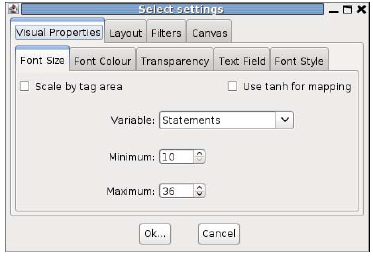
\includegraphics[scale=0.50]{old1.png}
  \caption{Mapping selection font size}
\end{subfigure}%
\begin{subfigure}{.5\textwidth}
  \centering
  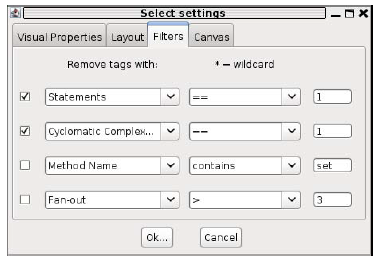
\includegraphics[scale=0.50]{old2.png}
  \caption{Tag filtering}
\end{subfigure}
\begin{subfigure}{\textwidth}
  \centering
  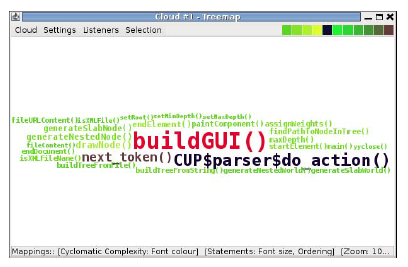
\includegraphics[scale=0.80]{old3.png}
  \caption{Canvas with tag cloud and colour chip legend}
\end{subfigure}%
\caption{\textit{Original Taggle prototype}}
\label{fig:original}
\end{figure}

In this research, I have extended and enhanced this prototype in order to create a stable system which could satisfactorily explore software quality assurance data such as metrics and code smells using tag cloud visualisation. Additionally, the possibility of using other software artefacts such as process management data and general multi-variate data, has been left open.

In the course of this research, changes were made to the original prototype which included:

\begin{itemize}
\item implementation of changes resulting from software engineering challenges and tag cloud visual variable analysis (Chapter~\ref{chap:tagcloud})
\item improvements generated from heuristic evaluation (Chapter~\ref{chap:heuristiceval})
\item implementation of an XML data conversion utility 
\item usability improvements and bug fixes
\end{itemize}

The software pictured and described in the rest of this chapter refer to the final prototype, after all alterations and improvements have been made.

\section{Data model and transformation}\label{sect:datamodel}

Source data for Taggle may be generated externally and provided in an XML format conforming to a DTD. There are a variety of tools/methods which can produce software metric data from static analysis of source code (such as that proposed by \citet{irwin03}, and see Appendix~\ref{appdx:tools} for a list of available plugins, software analysis platforms and frameworks/tools that can generate metric data). Most of these tools can output data into a CSV or XML format (\S\ref{sect:met}). I produced a tool to convert CSV formatted data to the Taggle XML format. This has also proved useful for conversion of datasets that may easily be obtained from external sources such as \url{www.findthedata.com}. Tools which produce XML formatted output only may also be transformed (using XSLT for example). 

The Taggle XML format specifies such things as measurement scales (nominal, ordinal and ratio) and relationships. Datasets consist of records (data points), each containing a number of fields. Visual mappings to properties and constraints for each data field can be specified via the GUI. Once the constraints of the visual property are set, a relative weighting for each tag is calculated according to the rank of the measurement. The calculation of rank is dependent on the measurement scale type. The weightings are used to calculate the value of the visual property for an individual tag, between the user defined constraints for a visual property (for example minimum and maximum font sizes). A full description of the Taggle XML format and weighting calculations can be found in \citet{deaker11c}.

As an example, consider the tag cloud in Figure~\vref{fig:activemqcamel}: the XML source file contained quality metrics from a subproject of open source project  ActiveMQ, the metrics were of the Chidamber and Kemerer suite generated by the CKJM toolkit. These were originally produced in space-separated text format, converted to CSV by OpenOffice, and then converted to the Taggle XML format by our conversion tool. In the GUI, the nominal field ``Class'' was mapped to the tag text (Arial font), the ratio field ``LCOM'' was mapped to the tag ordering property and the font size property (spanning from 20pt to 35pt), and the ratio field ``CBO'' was mapped to a background colour range from black to red. The tags have been positioned according to a simple tag cloud layout algorithm ``typewriter'', where the tags are mapped sequentially left to right, top to bottom (ways to improve the overall presentation are discussed later in the chapter). Default values for the visual mappings and other settings for Taggle can be controlled using an external XML file. 

\begin{figure}[!htb]
  	\centering
   	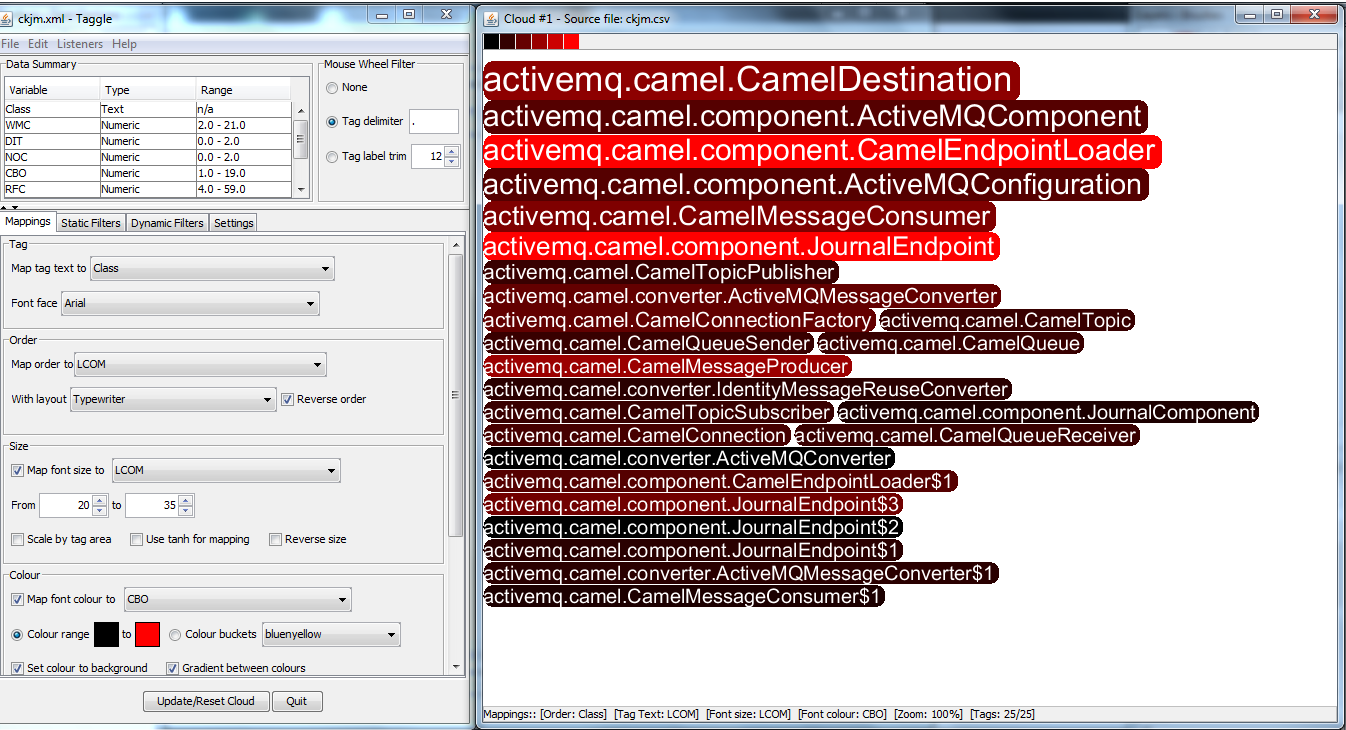
\includegraphics{activemqcamel.png}
  	\caption{\textit{A tag cloud generated by Taggle depicting a subproject of ActiveMQ with metrics derived from CKJM. Visual mapping interface is on the left.}}
	\label{fig:activemqcamel}
\end{figure}

\section{Visual encoding and mapping selection}\label{sect:visualencoding}

For brevity, only visual encoding and mapping features utilised in this research are discussed in this section. Information regarding other mapping properties and tag cloud layout algorithms can be found in the following technical documents: \citet{deaker11, deaker11c} (note that these documents describe the basic procedure which hasn't changed much, whereas the graphical interface, numbers of options, and features have changed significantly through the course of this research).

The mapping selection interface can be seen in Figure~\vref{fig:mappingselection}. In the analysis of visual properties available in tag clouds (Chapter~\ref{chap:tagcloud}), order, size, colour and transparency were deemed the most appropriate visual variables for data mapping purposes. The order in which they are displayed on the central mapping pane is in order of perceived usefulness and importance (with tag order being the most useful and transparency the least useful). By default, only the minimum mappings essential for display (tag and tag order) are turned on.

\begin{figure}[!htb]
\begin{subfigure}{.5\textwidth}
	\centering
	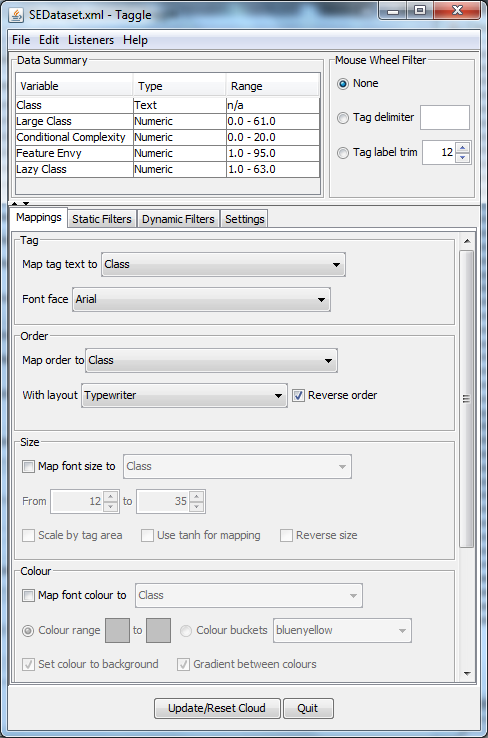
\includegraphics[scale=0.40]{mappings1.png}
	\caption{\textit{Data summary panel toggled on}}
\end{subfigure}%
\begin{subfigure}{.5\textwidth}
  \centering
  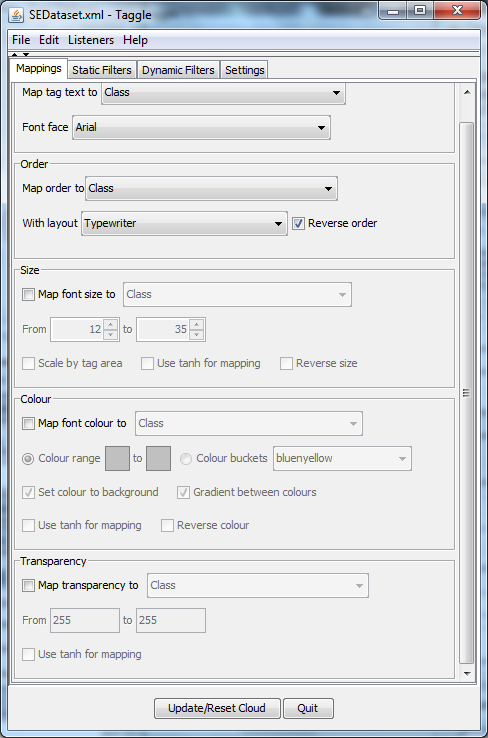
\includegraphics[scale=0.40]{mappings2.png}
  \caption{\textit{Data summary panel toggled off}}
\end{subfigure}
  \caption{\textit{Mapping selection interface: the data summary panel can be toggled by the user as desired to save valuable screen space}}
  \label{fig:mappingselection}
\end{figure}

The user is supported in the choice of appropriate mappings for the tag cloud by a data summary screen shown in a resizeable pane at the top of the GUI --- for an example see Figure~\vref{fig:datasummary}. Each field in the data file is shown along with data type (text, numeric or categorical) and the range of values in the category.  The data summary panel was included by request from a heuristic evaluation (see Chapter~\ref{chap:heuristiceval}).

\begin{figure}[!htb]
  	\centering
   	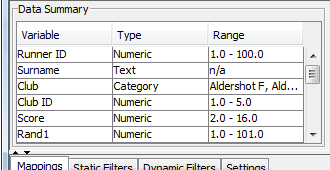
\includegraphics[scale=0.80]{datasummary2.png}
  	\caption{\textit{Closeup of an example data summary panel}}
	\label{fig:datasummary}
\end{figure}

\subsection{Categorical and continuous data}

Data types displayed in the data summary screen are determined programmatically. Fields are labelled categorical when the value ranges correspond to a certain maximum distinct number of values (the actual number is controlled via a setting). It is limited to a particular number of distinct values to match the number of colour chips displayed in the legend --- categorical variables are used predominantly in display colour mappings (\S\ref{colourmappings}). Providing a method for distinguishing these two types of data was included by request from the heuristic evaluation, where it was determined to be useful to display categorical data using a unique colour for each category.

\subsection{Tag}

\paragraph{Visual variable: tag length} The user is free to select any field to map to the tag text, including numeric types. The tag lengths for each tag will differ depending on the number of characters in the tag text. To minimise the possible effects on perception long textual identifiers may have, see \S\ref{sect:textualdata} for a description of the application of filters.

\paragraph{Visual variable: font family} The font face dropdown box is pre-populated with fonts that are installed on the machine running Taggle. Because reading ease is improved when presented with familiar fonts \citep[pg 106, chap 11:7][]{usability06}, Arial, Helvetica and Times New Roman (or the equivalents depending on the operating system and installed word processing software) are presented for selection at the top of the dropdown box, separated by a divider (see Figure~\vref{fig:fontfamily}).

\begin{figure}[!htb]
  	\centering
   	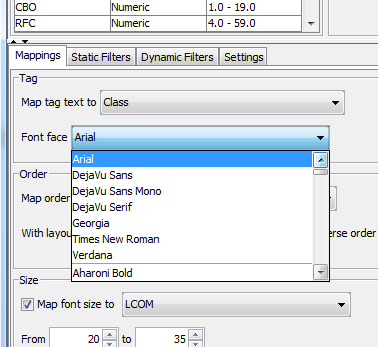
\includegraphics[scale=0.50]{fontfamily.png}
  	\caption{\textit{Prompting selection of familiar fonts.}}
	\label{fig:fontfamily}
\end{figure}

\subsection{Order}

\paragraph{Visual variable: order} If the order visual property is mapped to a field containing textual data, ordering of the tags is determined alphabetically, otherwise tags are ranked by their numerical value. The selected ordering can be reversed with the ``reverse order'' checkbox and updating the tag cloud. The user can select an appropriate layout from typewriter, spiral or force directed (defaulting to the simplest layout, typewriter).

\subsection{Size}

\paragraph{Visual variable: font size} Research has indicated slower reading performance for smaller font size \citep[pg 107, chap 11:8][]{usability06}, so there are constraints on the minimum font size to be set to no less than 9pt. The maximum font size is constrained to 250pt: by default this is set to a much smaller 35pt to allow for a smaller screen and canvas size (canvas size can be adjusted from the settings tab). The data mapped to the selected font sizes can be reversed with the ``reverse size'' checkbox.

\subsection{Colour and transparency} \label{colourmappings}

\paragraph{Visual variable: background colour} The heuristic evaluation and controlled experiments conducted in this research determined that the use of background colour was useful for visual search with colour mappings, as well as dataset features such as multiple word tags. Background colour has also been found to support more accurate estimation of relevant tags \citep{waldner13}. Therefore tag display via background colour is the default setting in Taggle. 

The user may select from a choice of colour range (between user defined colours) or colour buckets (a set palette of colours) --- see Figure~\vref{fig:colourinterface}. When the user chooses a data field to map to colour, colour range or colour bucket is automatically selected depending on whether the data field is categorical data. Categorical data is best displayed through a unique set of colours preselected from a colour palette (the colour palettes can be user defined through external string property files, although default palettes are provided.) For example, in Figure~\vref{fig:colourbuckets} a dataset about agile projects is displayed in a tag cloud. With the aim of finding what actors are related to the agile stories with the highest time estimates, order/size are mapped to estimate and colour is mapped to actor. The user can determine stories with the greatest estimated workload corresponding to tags coloured dark grey and brown, and find details via a colour legend mouse hover or tag label mouse hover (actors `Preferred customer' or `Bookstore customer').

Continuous data is best displayed through a colour range. The user has the option of choosing a colour gradient between two selected colours, or colours which appear on the colour wheel between two selected colours (see Figure~\vref{fig:continuous}. Colour models are complicated and won't be discussed in full detail). Like other mappings, the user also has the option to reverse the selected mappings so high values can be shown with the `from' colour and low values can be shown with the `to' colour.

\begin{figure}[!htb]
  	\centering
   	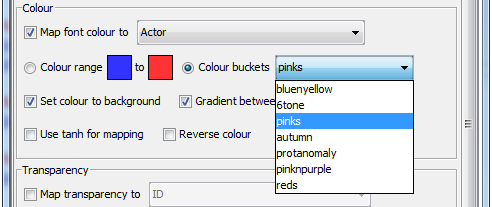
\includegraphics[scale=0.75]{colourinterface.png}
  	\caption{\textit{Colour mapping interface}}
	\label{fig:colourinterface}
\end{figure}

\begin{figure}[!htb]
\begin{subfigure}{.5\textwidth}
	\centering
	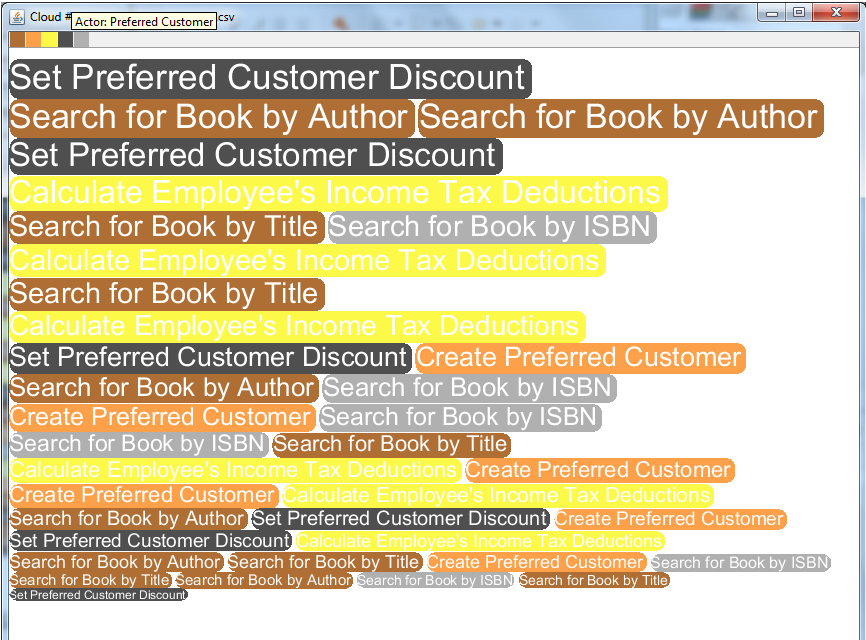
\includegraphics[scale=0.20]{colourbuckets1.png}
	\caption{\textit{Mouse over the legend}}
\end{subfigure}%
\begin{subfigure}{.5\textwidth}
  \centering
  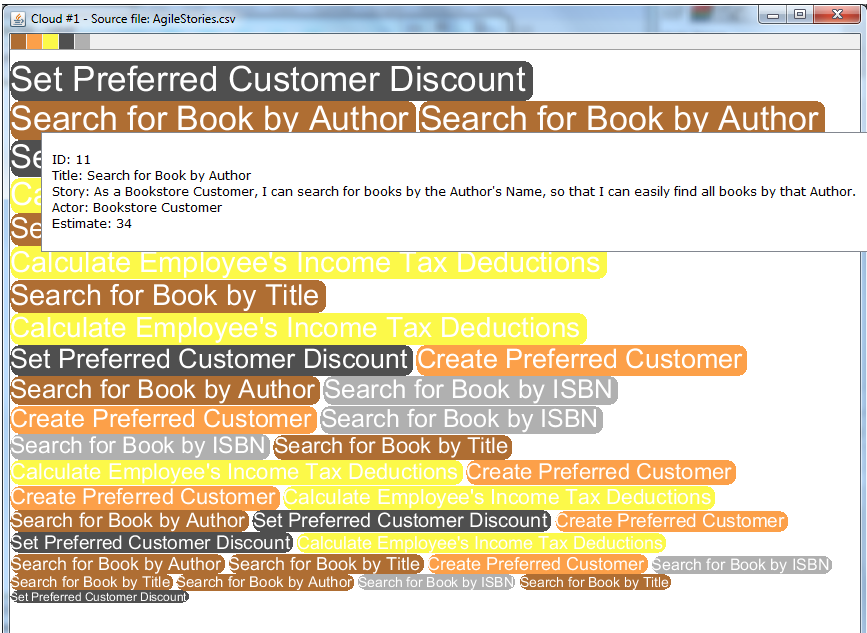
\includegraphics[scale=0.20]{colourbuckets2.png}
  \caption{\textit{Mouse over a tag}}
\end{subfigure}
  \caption{\textit{Displaying categorical data with colour buckets}}
  \label{fig:colourbuckets}
\end{figure}

\begin{figure}[!htb]
\begin{subfigure}{.5\textwidth}
	\centering
	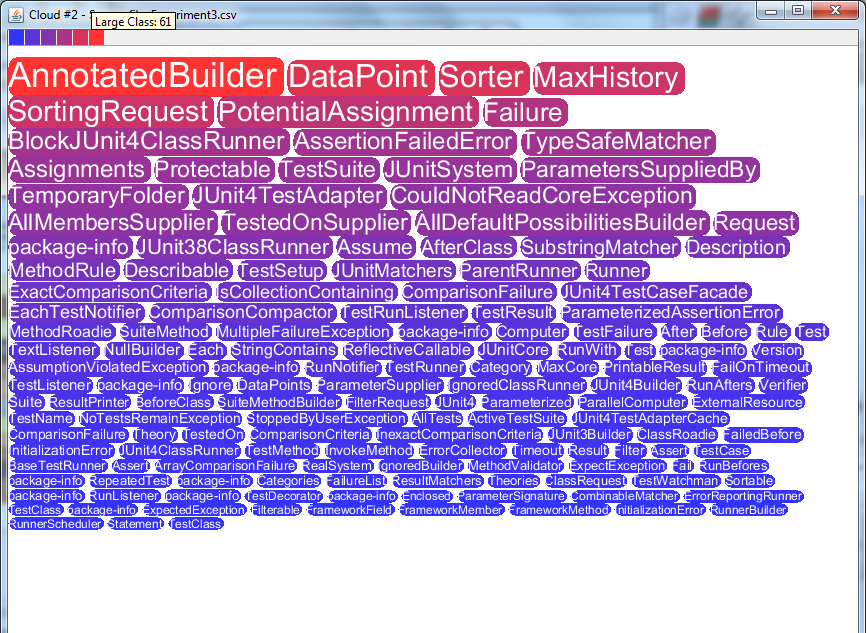
\includegraphics[scale=0.20]{colourbuckets3.png}
	\caption{\textit{Colour gradient between red and blue}}
\end{subfigure}%
\begin{subfigure}{.5\textwidth}
  \centering
  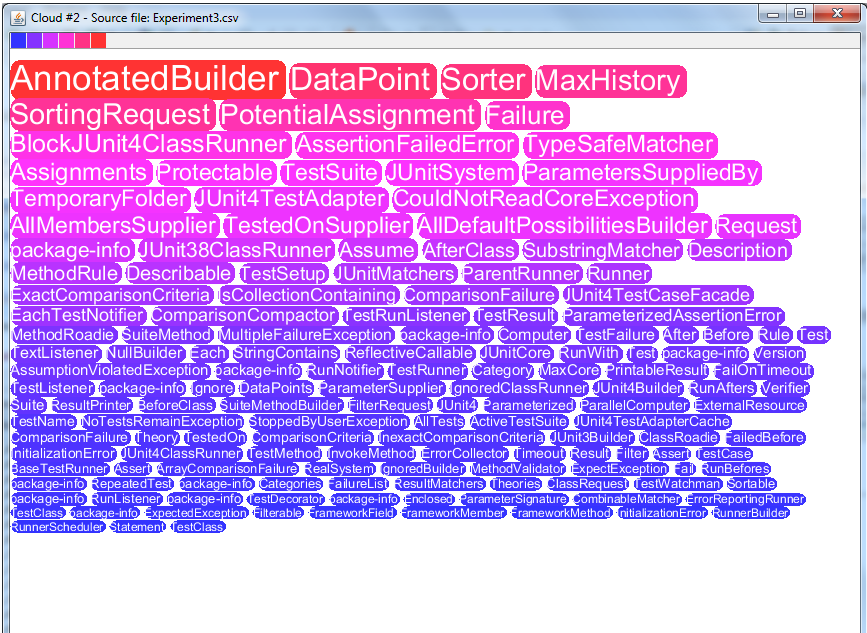
\includegraphics[scale=0.20]{colourbuckets4.png}
  \caption{\textit{Colour wheel between red and blue}}
\end{subfigure}
\begin{subfigure}{\textwidth}
  \centering
  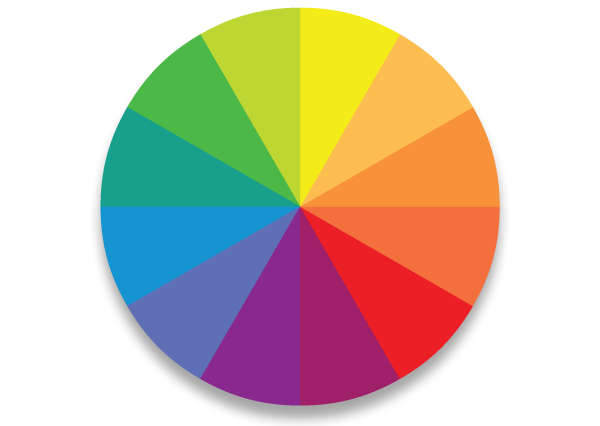
\includegraphics[scale=0.40]{colour_wheel.png}
  \caption{\textit{A colour wheel}}
\end{subfigure}
  \caption{\textit{Displaying continuous data with colour ranges}}
  \label{fig:continuous}
\end{figure}

\paragraph{Visual variable: font colour} The user also has the choice of displaying a more conventional looking tag cloud, with colour mapped to the font rather than the background (see Figure~\vref{fig:fontcolour}).

\begin{figure}[!htb]
  	\centering
   	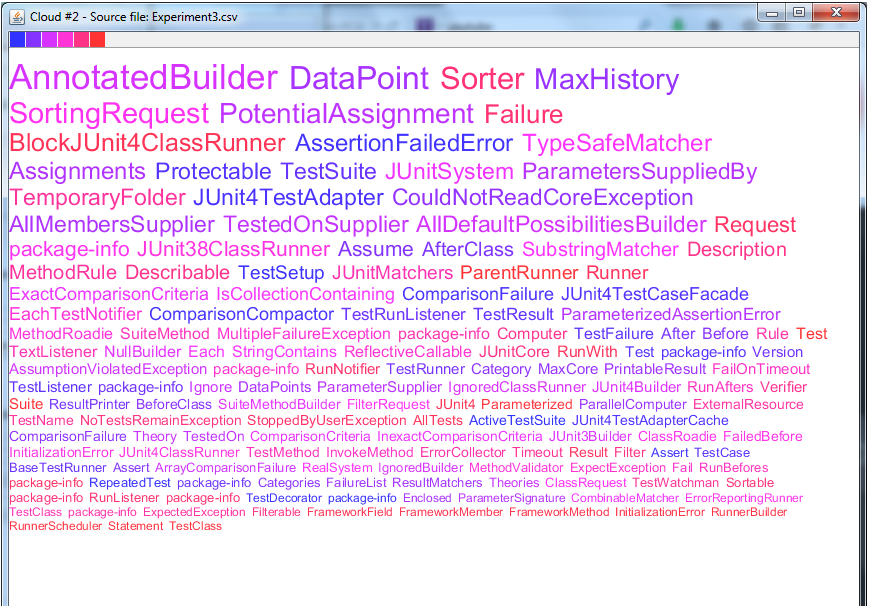
\includegraphics[scale=0.35]{fontcolour.png}
  	\caption{\textit{Colour mapped to the font}}
	\label{fig:fontcolour}
\end{figure}

\paragraph{Visual variable: transparency} The user may map data fields to a visual property which is familiarly used in tag clouds online --- transparency --- see Figure~\vref{fig:transparency}. This can be applied with or without colour.

\begin{figure}[!htb]
\begin{subfigure}{.5\textwidth}
	\centering
	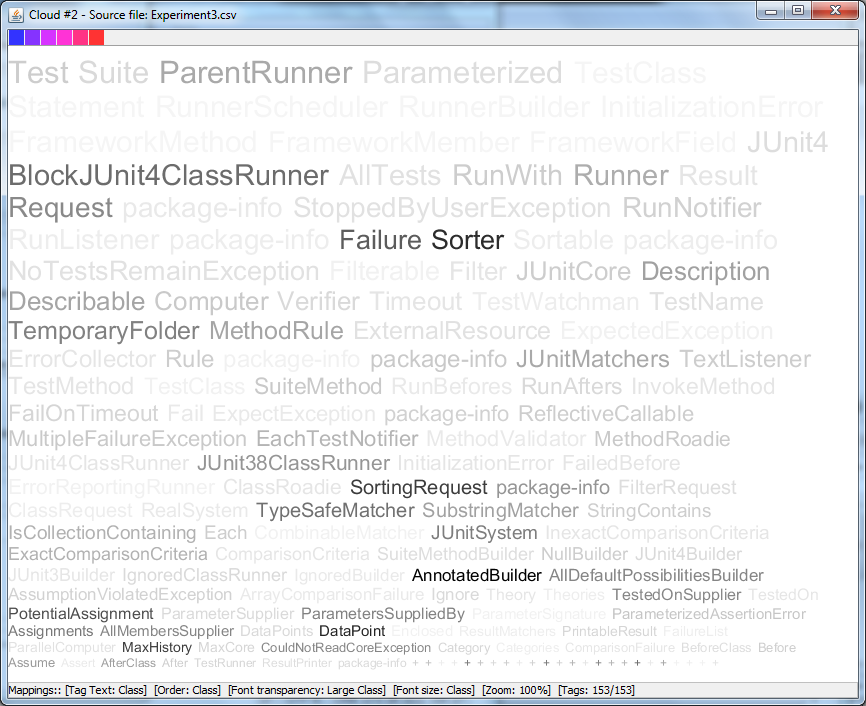
\includegraphics[scale=0.20]{transparency.png}
	\caption{\textit{Without colour applied}}
\end{subfigure}%
\begin{subfigure}{.5\textwidth}
  \centering
  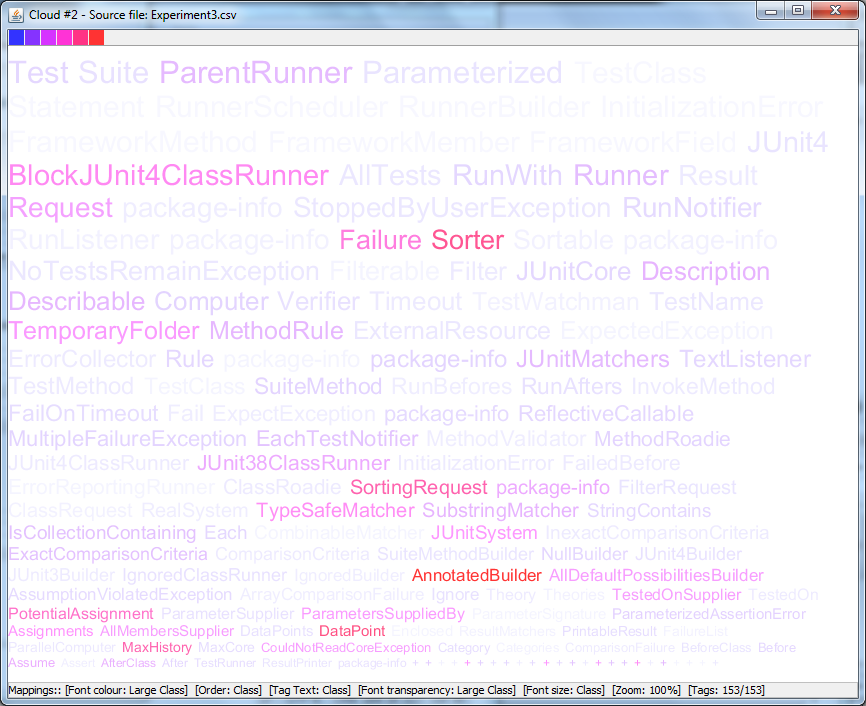
\includegraphics[scale=0.20]{transparency2.png}
  \caption{\textit{With colour applied}}
\end{subfigure}
  	\caption{\textit{Transparency mapping}}
	\label{fig:transparency}
\end{figure}

%\subsection{Bertin's visual variables}

%Chosen mappings are selective and associative. Quantitative issues - comparisons using mouse drags.

\section{Software engineering tasks}\label{sect:softwaretasks}

Taggle includes a number of interactive features to enable rich data exploration. Only the features which were utilised in this research and pertain directly to completing the software engineering tasks outlined in \S\ref{sect:tasktypes} are described in this section. For further information describing features such as relationship highlighting, cloud listeners, sub-clouds and linking, see technical documents: \citet{deaker11, deaker11c}.

\subsection{Filtering textual data}\label{sect:textualdata}

Textual data is an issue with some multi-variate data visualisation techniques such as treemaps or scatterplots because of issues with screen real estate. On the other hand, a tag cloud is designed to include the (often important and identifying) textual data as a key part of the graphic. Software textual data is often in the form of long identifiers such as class or agile story names. Taggle's mouse wheel filtering (used for textual data displayed in the tag, interface shown in Figure~\vref{fig:filtering1}) can be used to dynamically select the portions of the text identifier that the user deems most important and/or maximise the available visualisation space. When the `Tag delimiter' option is selected, the user may filter the text by a particular character by scrolling the mouse wheel (scrolling up filters off leading text while scrolling down filters off trailing text). In Figure~\vref{fig:filtering2} you can see an example of typical software engineering data displaying Java package and class names as the textual identifier in the text with a) showing the original tag text and b) text filtered to two packages above the class name.

\begin{figure}[!htb]
  	\centering
   	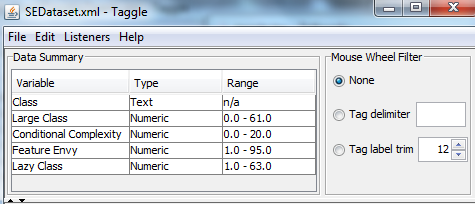
\includegraphics[scale=0.75]{mousefilter.png}
  	\caption{\textit{Mouse filtering interface}}
	\label{fig:filtering1}
\end{figure}

\begin{figure}[!htb]
\begin{subfigure}{\textwidth}
	\centering
	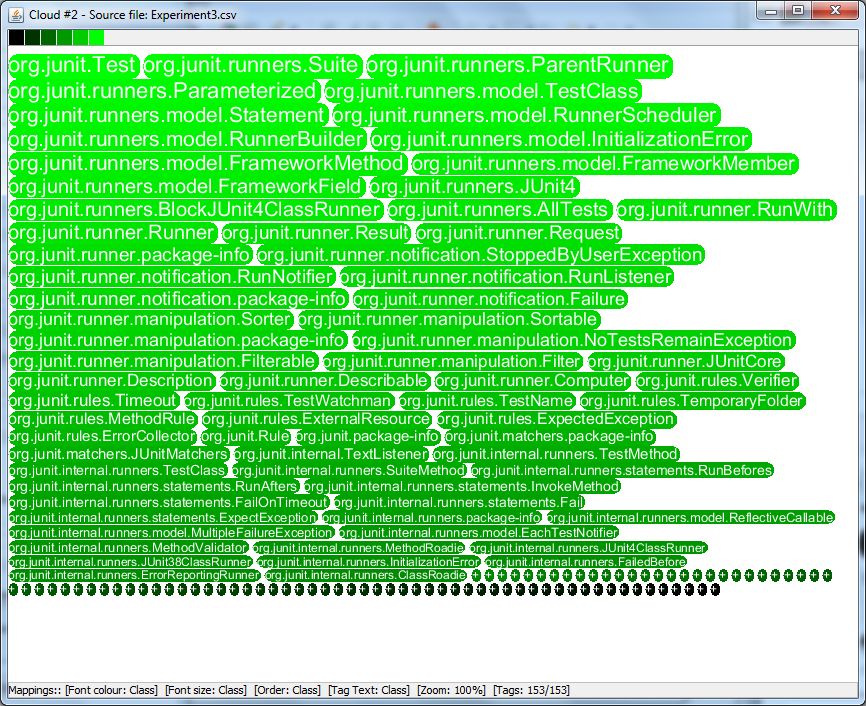
\includegraphics[scale=0.35]{delimiterfilter1.png}
  	\caption{\textit{Original tag text}}
\end{subfigure}
\begin{subfigure}{\textwidth}
 	 \centering
	 \includegraphics[scale=0.35]{delimiterfilter2.png}
	 \caption{\textit{Filtered on a `.' delimiter}}
\end{subfigure}
  \caption{\textit{Filtering on a character delimiter}}
  \label{fig:filtering2}
\end{figure}

The user also has the option of filtering the text to a fixed number of characters from either the leading or trailing text (Figure~\vref{fig:filtering3}). This has two purposes, to maximise available real estate in the canvas, and to minimise any effect a greater number of characters in a tag may have on user perception. This filter can be used in combination with removing the font size mapping selection, which further minimises bias in eye attention.  

\begin{figure}[!htb]
  	\centering
   	\includegraphics[scale=0.35]{taglabeltrimfilter.png}
  	\caption{\textit{Filtering on a fixed number of characters from the leading text}}
	\label{fig:filtering3}
\end{figure}

\subsection{Dealing with large scale data}

One feature of software engineering datasets is that there is often a large number of data points to contend with, and any potential visualisation tool must provide a mechanism to deal with this. Using the ``Information Seeking Mantra'' \citep{schneiderman96}, we first provide the user with an overview of the dataset (see Figure~\vref{fig:detailsondemand}), and allow additional details to be accessed on demand via a mouse hover. As seen in Figure~\vref{fig:filtering2}, tag labels too long to be displayed on the canvas are minimised into symbols. This has the advantage that they don't disappear from view together, and hovering over the iconified form reveals their details. As the user interacts with the data using filtering and dynamic queries, these symbols are transformed into textual labels as canvas real estate becomes available. 

\begin{figure}[!htb]
  	\centering
   	\includegraphics[scale=0.35]{detailsondemand.png}
  	\caption{\textit{Overview first, then details-on-demand}}
	\label{fig:detailsondemand}
\end{figure}

Filtering can be applied to the dataset (Figure~\vref{fig:staticfilter}) to narrow the view as desired, or dynamic querying (Figure~\vref{fig:taggledynamicfilter}) where the user is able to see the tags filtered from display in real time using a range slider. 

\begin{figure}[!htb]
  	\centering
   	\includegraphics[scale=0.30]{staticfilter.png}
  	\caption{\textit{Applying filtering to the data}}
	\label{fig:staticfilter}
\end{figure}

\begin{figure}[!htb]
  	\centering
   	\includegraphics[scale=0.30]{dynamicfilter.png}
  	\caption{\textit{Dynamic querying}}
	\label{fig:taggledynamicfilter}
\end{figure}

It is also possible to display an overview of data while allowing detailed information to be shown simultaneously with a zoom function (Figure~\vref{fig:zoom}). A particular concern using the tag cloud technique is lack of space due to long label lengths, or many labels with a large dataset. In this case the user may apply dynamic mouse wheel filtering and label trimming as detailed in \S\ref{sect:textualdata}.

\begin{figure}[!htb]
  	\centering
   	\includegraphics[scale=0.40]{zoom.png}
  	\caption{\textit{Zoom in on a small area}}
	\label{fig:zoom}
\end{figure}

\subsection{Identify similar characteristics of data}

Similar data characteristics can be identified using filtering and details-on-demand. In Figure~\vref{fig:cluster}, a user inspects the classes with a low level of the `lazy class' metric within a software dataset. Using either dynamic queries or details-on-demand on the filtered dataset it is possible to establish that classes with a low level of `lazy class' also have a low level of metric `feature envy' (refer to Chapter~\ref{chap:exp3} for further details regarding this example dataset). Following this kind of filtered inspection, a user might make use of a visual property mapping such as colour to identify a data correlation between the two variables (see \S\ref{sect:datacorrelation}).

\begin{figure}[!htb]
  	\centering
   	\includegraphics[scale=0.30]{cluster1.png}
  	\caption{\textit{Using filtering to identify similar data characteristics}}
	\label{fig:cluster}
\end{figure}

\subsection{Identifying data distribution}

The distributions of variables in software engineering metric datasets are often heavily skewed (see Figure~\vref{fig:distributions} for some graphical examples of this). In Taggle, colour and order are mapping choices which can be applied to the data in order to highlight data distribution. In Figure~\vref{fig:distribution}, the metric `large class' is being visualised from a software project. To avoid bias in user perception, font size is unmapped and the tag labels have been filtered to a fixed length. The ordering of the tags is arranged in order of the metric in question, from largest value to smallest. A colour gradient between green and black is also mapped to `large class', where black identifies tags which have the lowest levels of `large class', and green shows tags with the highest levels. The distribution of colour across the visualisation shows the user that values of `large class' are skewed towards the lower end as expected. As a user of Taggle, the classes that would now become of interest as possible candidates for refactoring would be the few brightest green tags to the top left.

\begin{figure}[!htb]
  	\centering
   	\includegraphics[scale=0.40]{distribution.png}
  	\caption{\textit{Using colour to identify data distribution of the `large class' metric}}
	\label{fig:distribution}
\end{figure}

\subsection{Identify data correlations and outliers}\label{sect:datacorrelation}

Software metric data distributions are typically heavily skewed and may contain outliers. In statistics, outliers are often discarded or ignored during analysis: in software engineering these outliers are often points of interest. In Figure~\vref{fig:correlation}, colour and order are used to investigate a possible correlation between data variables, metrics `lazy class' and `feature envy'. Size and order are dually mapped to `feature envy' while a colour range (blue to red) is mapped to `lazy class'. We see that as the font size becomes smaller, the colour mapping changes gradually from red to blue in a progressive fashion. This is indicative of a correlation between the two variables. There are three data points which have colouring that stands out amongst the rest (classes `Enclosed', `Theory' and `JUnit4TestAdapter'), these points may appear as outliers in the correlation between the data variables. In Figure~\vref{fig:correlation1}, colour is scattered without pattern across the order and font size, no correlation can be seen between variables `conditional complexity' and `feature envy'.

\begin{figure}[!htb]
  	\centering
   	\includegraphics[scale=0.30]{correlation.png}
  	\caption{\textit{Using colour to identify a data correlation and outliers}}
	\label{fig:correlation}
\end{figure}

\begin{figure}[!htb]
  	\centering
   	\includegraphics[scale=0.30]{correlation1.png}
  	\caption{\textit{No data correlation between variables}}
	\label{fig:correlation1}
\end{figure}

\subsection{Finding minimum/maximum values}

In software metric analysis, finding classes which hold the minimum or maximum values of a metric is useful for identifying classes that are candidates for refactoring. The order mapping, or a dual mapping of order and font size, are useful for identifying classes in the lower and upper boundaries. In Figure~\vref{fig:minimum1}, `AnnotatedBuilder' and `DataPoint' classes are easily identified as having the highest values of the `conditional complexity' metric when dually mapped to order and font size.

\begin{figure}[!htb]
  	\centering
   	\includegraphics[scale=0.40]{minimum1.png}
  	\caption{\textit{Finding classes with the highest value of a metric using \\dual order and font size mappings}}
	\label{fig:minimum1}
\end{figure}

\subsection{Comparison of data elements}

Comparison of data points is another key task useful in any software engineering or multi-variate dataset. In Figure~\vref{fig:minimum1} font size and order are dually mapped to field `conditional complexity'.  It is obvious for example, that tag `JUnitSystem' has a higher conditional complexity than tag `JUnitMatchers'. When font size and order are not mapped to the same data field it may not be so obvious. Using drag and drop a user may pull out the relevant tags and put them next to one another for easier comparison --- see Figure~\vref{fig:comparison}. Additionally, a user may hover over the tags and view the class metric information in the pop-up details-on-demand for comparison.

\begin{figure}[!htb]
  	\centering
   	\includegraphics[scale=0.35]{comparison.png}
  	\caption{\textit{Comparison of `JUnitSystem' and `JUnitMatchers'}}
	\label{fig:comparison}
\end{figure}

\section{Summary and discussion}

In this chapter, we introduced the tag cloud visualisation tool Taggle. This tool was inherited from previous research and extensively modified to create a stable system able to explore software quality metrics and other more general multi-variate data. Most notably, a variety of implementation changes were made as a result of considering design aspects from software engineering and tag cloud visual variable analysis (Chapter~\ref{chap:tagcloud}) as well as improvements generated from a heuristic evaluation by domain experts (Chapter~\ref{chap:heuristiceval}).

Data can be gathered from a variety of sources and then converted (through XML transform or conversion utility) into a special Taggle XML format. This XML file is then input into Taggle through the user interface, where the user can view generated tag clouds and customise the visual property mappings as they explore the dataset. Interface and visual encoding design choices such as the visual properties included, constraints and options for each property, and filtering selections were made with respect to the software engineering and design considerations listed in previous chapters. Some choices, such as the data summary screen and categorical data options, were incorporated by request during the heuristic evaluation.

In Chapter~\ref{chap:tagcloud}, a list of tasks was presented that represented meaningful ways users could interact with software data. These included tasks from data mining task types --- clustering, summarising,  associating and classifying --- and involved activities such as identifying similar data characteristics, distribution and correlations. In \S\ref{sect:softwaretasks}, we showed how a user could interact with a sample software engineering dataset to complete each task using the system. Taggle's design was intended to cope specifically with the challenges of software engineering datasets, by using appropriate visual mappings available in tag clouds to render the data.

% ------------------------------------------------------------------------


%%% Local Variables: 
%%% mode: latex
%%% TeX-master: "../thesis"
%%% End: 


%Systematic mapping study of evaluation
\chapter[Systematic Mapping Study of Tag Cloud Research]{Systematic Mapping Study\\of Tag Cloud Research}

\label{chap:strateval}
\ifpdf
    \graphicspath{{Chapters/SystematicMappingStudy/SystematicMappingStudyFigs/PNG/}{Chapters/SystematicMappingStudy/SystematicMappingStudyFigs/PDF/}{Chapters/SystematicMappingStudy/SystematicMappingStudyFigs/}}
\else
    \graphicspath{{Chapters/SystematicMappingStudy/SystematicMappingStudyFigs/EPS/}{Chapters/SystematicMappingStudy/SystematicMappingStudyFigs/}}
\fi


Information visualisation techniques can be challenging to evaluate \citep{plaisant04}. This is because, in addition to general evaluation challenges (such as choosing appropriate questions and tasks, defining methods and then executing the evaluation correctly) the visualisation focus on the data exploration process is difficult to capture and quantify. We embarked on a systematic mapping study of previous research evaluating the tag cloud technique or interactive tools that included tag cloud visualisation. This study identified topics, fields or domains that had not been extensively researched, and approaches and methods which had been used for evaluation. To classify our work, we used a set of information visualisation guiding scenarios which are outlined in \S\ref{sect:strategies}. Research questions and goals for the study are presented in \S\ref{sect:researchquestions}. The research methodology including data sources, study selection and data extraction are outlined in \S\ref{sect:mappingmethods}. Results for research topic, methods, domains and approaches are discussed in \S\ref{sect:mappingresults}. Finally, summary and conclusions are presented in  \S\ref{sect:mappingdiscussion} and \S\ref{sect:mappingconclusions}. 

%This work provided an overview of what is known about tag clouds, and helped us plan and focus our overall evaluation strategy.

\section{Strategies for evaluation}\label{sect:strategies}

In 2012, \citet{lam12} identified seven guiding scenarios for information visualisation evaluation. These scenarios were gathered from a systematic review of 803 information visualisation papers (345 of which included evaluations). Of these scenarios, four can be roughly defined as evaluation of the \emph{data analysis process} (EWP, VDAR, CTV, CDA -- described in \S\ref{sect:dataextraction}) and the remaining three evaluate the \emph{visualisation use} (UP, UE, VA). These two types of strategies have different goals and use different methodologies. 

Evaluation of the \emph{data analysis process} has a goal of understanding the underlying process and roles played by the visualisation itself, and captures a more whole-tool holistic view. The results from this type of analysis may be more meaningful as realistic tasks and scenarios are used. However, results can be more difficult to quantify. Also, the whole tool is evaluated so evaluation may require full featured and mature tool.

The \emph{visualisation use} type strategies do not evaluate the whole tool but a system slice or technique. They are used to evaluate design decisions, explore the design space, benchmark existing systems or test usability. For these strategies, outputs are easier to quantify generated insight. There is a need to break the evaluation into techniques or visual encoding types, so careful prioritisation is needed. Because of this breaking off into sections, more than one experiment may be needed. Tasks may also need to be heavily abstracted which impacts realism.

In the systematic review performed by \citet{lam12}, only 15 percent of papers used data analysis process type strategies in their evaluation. They concluded that evaluation in the information visualisation sector has been following in the footsteps of evaluations for Human Computer Interaction (HCI) and Computer Graphics (CG), both of which are traditionally focused on controlled experiments and usability evaluations. The data process strategy research questions (such as a tools support for reasoning, knowledge discovery or decision making) are of high relevance and practical value. \citet{lam12} highlighted the need to think critically about the goals of the types of evaluations needed for information visualisation.

We were interested to find out what types of evaluations had been performed for tools utilising tag cloud visualisation techniques, and what research topics and domains the evaluations focused on so we performed a systematic mapping study on 60 selected primary studies from 2007 to 2012. 

%We found that 93\% of evaluations used visualisation use type strategies. This was despite 43\% of papers incorporating tag clouds (or enhanced tag clouds) into interactive systems which likely had goals of exploring data or discovering information. Research was strongly focussed in the WWW domain. 

\section{Systematic mapping study}\label{sect:researchquestions}

We had a number of goals for our systematic mapping study. We wanted to find all papers which have evaluated the effectiveness of the tag cloud visualisation technique in order to identify those areas of tag cloud visualisation which contain either exhaustive research (allowing us to apply and build on), or deserts of information (allowing us to shape future research in this area). Secondly, tag clouds are most commonly associated with the web - we were interested to find out what other domains had proposed and evaluated tag cloud visualisation techniques. Finally, we wanted to discover what evaluation approaches and methods had been used by tag cloud evaluation studies in order to achieve their research goals. Overall, the systematic mapping study should serve to build an overview of what is known about tag clouds as a visualisation technique in general, identifying clusters of evidence and establishing areas of research where knowledge gaps exist. 

\begin{description}
\item[RQ:] \textit{What topics for tag cloud visualisation have been evaluated and to what extent?} We want to establish which topic areas have been focused on in previous research, in order to help shape future research.
\item[RQ:] \textit{What evaluation approaches and methods have been used?} We want to discover what types of evaluation have been undertaken for tag cloud visualisation, and what methods were used.
\item[RQ:]\textit{ For which fields or domains have tag cloud visualisations been evaluated?} The domain which tag clouds are primarily associated with is the web. We want to know what other fields or domains tag cloud visualisation has been proposed and evaluated for. 
\end{description}


%\section{Research Questions}\label{researchquestions}
%\input{Chapters/SystematicMappingStudy/researchquestions}

\section{Methods}\label{sect:mappingmethods}
%Scope of the study is as follows:
%\begin{itemize}
%\item Population: Published scientific literature reporting on information visualisation.
%\item Intervention: Research including an evaluation of tag cloud visualisation.
%item Outcomes of relevance: Quantity and type of evidence relating to tag clouds as a visualisation or user interface.
%\item Experimental design: Any scientific experiment or empirical study.
%\end{itemize}
During the course of the systematic mapping study, the following activities were carried out: define research questions, define data sources and search strategy, perform searches in all designated digital libraries and search engines using the filter, remove duplicate studies (results reported from multiple search engines), review each paper using specified inclusion/exclusion criteria and determine relevance to the topic and research questions, perform data extraction, and perform data synthesis.

\subsection{Data sources and search strategy}

The digital libraries and search engines which were used to extract the articles were ACM digital library\footnote{\url{dl.acm.org/}},  IEEE Explore\footnote{\url{ieeexplore.ieee.org}}, SpringerLink\footnote{\url{www.springerlink.com}}, CiteSeer\footnote{\url{citeseerx.ist.psu.edu/}}, Scopus\footnote{\url{www.scopus.com}}, Sage Journals\footnote{\url{online.sagepub.com/}}, Scirus\footnote{\url{www.scirus.com}}, Web of Science\footnote{\url{wokinfo.com/}}, ScienceDirect\footnote{\url{www.sciencedirect.com/}} and arXiv\footnote{\url{arxiv.org/}}.

The search terms were grouped into three categories 1) pertaining to visualisation technique 2) relating to visualisation type and 3) search terms relating to evaluation.

\pagebreak

\begin{verbatim}
("tag cloud" OR "tag clouds" OR "tagcloud" OR "tagclouds") AND
("evaluation" OR "qualitative" OR "quantitative"
OR "experiment" OR "experimentation" OR "experiments"
OR "study" OR "studies") AND 
("visualisation" OR "visualization" OR 
"user interface" OR "user interfaces")
\end{verbatim}

These search groups were joined together with the use of a boolean AND to search document metadata (where available) such as title, abstract, classification and keywords. Additionally, each query had to be adapted according to the interface and query specification of the search engine.

In order to validate the search strategy, a check was performed to ensure a small sample of papers (12) was included in the search results \citep[][]{bateman08, hearst08, kaser07, lohmann09, oosterman10, rivadeneira07, schrammel09, schrammel09b, seifert08, kuo07, halvey07, sinclair08}. These papers had previously been noted as relevant to the research questions during an initial review of the literature.

\subsection{Primary study selection}
Each paper returned from the digital libraries and search engines using the specified query was checked for duplication against other database results. An initial result total of 181 was whittled down to 100 after removal of duplicates (see Table~\vref{tab:searchresults1}).

\begin{table}
\centering
\caption{\textit{Initial search results from digital libraries and corresponding duplicates}}
\begin{tabular}{|l|c|c|c|} \hline
\textbf{Digital Libraries}&\textbf{Results}&\textbf{Duplicates}&\textbf{Total}\\ \hline
ACM digital library&16&1&15\\ \hline
IEEE Explore&38&0&38\\ \hline
SpringerLink&10&0&10\\ \hline
CiteSeer&2&2&0\\ \hline
Scopus&70&55&15\\ \hline
Sage Journals&2&2&0\\ \hline
Scirus&0	&0&0\\ \hline
Web of Science&40&19&21\\ \hline
ScienceDirect&2&2&0\\ \hline
arXiv&1&0&1\\ \hline
\textbf{Totals}&\textbf{181}&\textbf{81}&\textbf{100}\\
\hline\end{tabular}
\label{tab:searchresults1}
\end{table}

Each paper was then checked for relevancy using the title, abstract and keywords. Studies that met one of the following inclusion criteria were included: 

\begin{itemize}
\item studies describing the evaluation of tag cloud visualisation
\item studies describing the evaluation of a visualisation or user interface based on the tag cloud technique
\item studies describing the evaluation of a system which utilises tag cloud visualisation 
\item studies describing the evaluation of a system which utilises a visualisation or user interface based on the tag cloud technique
\end{itemize}

Studies that met one of the following exclusion criteria were excluded:

\begin{itemize}
\item studies where only an abstract was available
\item studies where the paper was not available in English
\item studies describing the evaluation of a system where the evaluation method did not specifically include the tag cloud component
\item studies where the described evaluation served as a proof of concept
\item duplicate articles of the same study from different sources
\end{itemize}

In many cases it was not possible to determine relevancy of the study from the abstract alone, particularly in determining whether the evaluation method actually included evaluation of the tag cloud component of a system. For these studies, it was necessary to consider the paper as a whole. Each paper was reviewed twice for inclusion/exclusion criteria, during two passes of the search results as a means of validation. During the second review of the paper, a set of keywords was extracted. These served as the basis for the creation of the classification categories within mapping facets.

During the inclusion/exclusion phase a further 40 documents were excluded from the study, bringing the total number of primary papers included to 60 (see Table~\vref{tab:searchresults2} for the exclusion details, after duplicates had been removed).

\begin{table}
\centering
\caption{\textit{Search results from digital libraries and corresponding excluded papers}}
\begin{tabular}{|l|c|c|c|} \hline
\textbf{Digital Libraries}&\textbf{Results}&\textbf{Excluded}&\textbf{Total}\\ \hline
ACM digital library&15&1&14\\ \hline
IEEE Explore&38&22&16\\ \hline
SpringerLink&10&4&6\\ \hline
Scopus&15&8&7\\ \hline
Web of Science&21&5&16\\ \hline
arXiv&1&0&1\\ \hline
\textbf{Totals}&\textbf{100}&\textbf{40}&\textbf{60}\\
\hline\end{tabular}
\label{tab:searchresults2}
\end{table}

\subsection{Data extraction}\label{sect:dataextraction}

For each research question, a set of classification categories was devised within a mapping facet.

For RQ \textit{Research topic}, we determined the categories by extracting keywords from the primary studies:

\begin{itemize}
\item evaluating the effectiveness of the tag cloud technique
\item determining perceived physical demand or workload
\item proposal of evaluation metrics or methodologies
\item making design guidelines or recommendations
\item determining support for user process (social navigation, incidental learning, reflections of learners, determining credibility of sources, dynamic representation of places/situations)
\item discovering limits of visual perception (visual features or properties, layout)
\item determining user motivation for use
\item proposal of a tag cloud enhancement (with respect to relationships, topic clustering, temporal evolution, tag ranking algorithms, tagging interfaces, interfaces for a special dataset or medium, layout optimisation)
\item evaluations of systems/visualisations targeting a special population (Chinese readers, Hebrew readers, tools for the blind)
\end{itemize}

For RQ \textit{Evaluation approaches and methods}, the Seven Guiding Scenarios for Information Visualisation Evaluation proposed by \citet{lam12} were used to classify the evaluation approaches and methods:

\begin{description}
\item[EWP:] \emph{Understanding Environments and Work Practices.} Studying the design context for visualisation tools including tasks, work environments, and current work practices. Types of research methods include field observation, interviews and laboratory observation.
\item[VDAR:] \emph{Evaluating Visual Data Analysis and Reasoning.} Discovering if and how a visualisation tool supports the generation of actionable
and relevant knowledge in a given domain. Types of research methods include case studies and controlled experiments.
\item[CTV:] \emph{Evaluating Communication Through Visualisation.} Discovering if and how communication can be supported by visualisation (for example through learning, teaching, idea presentation and casual consumption of ambient displays). Types of research methods include controlled experiments and field observation and interviews. 
\item[CDA:] \emph{Evaluating Collaborative Data Analysis.} Studying whether a tool allows for collaboration, collaborative analysis, and/or collaborative decision-making processes. Types of research methods include heuristic evaluation, log analysis and field or laboratory observation.
\item[UP:] \emph{Evaluating User Performance.} Studying if and how specific visualisation features affect objectively measurable user performance. Types of research methods include controlled experiments and field logs.
\item[UE:] \emph{Evaluating User Experience.} People's subjective feedback and opinions.  Types of research methods include informal evaluation, usability tests and field observation.
\item[VA:] \emph{Evaluating Visualisation Algorithms.} Study the performance and quality of visualisation algorithms by judging the generated output. Types of research methods include algorithmic performance measurement and quality metrics.
\end{description}

By classifying the studies based on these guiding scenarios we get a picture of the underlying evaluation goals, rather than just a description of the type of research methods employed. 

For RQ \textit{Visualisation domain}, the categories were again determined by keywords we extracted from the primary studies:

\begin{itemize}
\item web (user generated content, database search results, recommendation systems)
\item mixed media (image, film, television and audio)
\item software engineering
\item text corpora
\item geographical information
\item mobile phone
\item digital forensics
\item health and medicine (online forums, tool for the blind)
\item situated displays
\item database search results (OLAP, online database)
\item multi-variate data
\end{itemize}

Papers may cover more than one domain or topic so can be associated with multiple classification types. Where applicable, papers were categorised into sub-topics (as indicated within the brackets).


\section{Results}\label{sect:mappingresults}

The distribution of primary papers over time can be seen in Figure~\vref{fig:barchart1} --- papers span from 2007 to 2012 (the mapping study was conducted 2012). Figure~\ref{fig:bubble1} shows a bubble chart of the mapping facets research topic and evaluation method. The totals do not match exactly with the total number of papers included in the study as it is possible for papers to cover both multiple topics and use multiple evaluation methods within the study. This is particularly common where studies use the evaluation approach UP (measuring user performance) as this evaluation method tends to use controlled studies and a corresponding UE (user evaluation) component, such as a lab questionnaire requesting subjective user feedback. It is possible to see in this chart a heavy tendency towards UP and UE evaluation approaches within the domains of text corpora and web. The focus on web and text is not surprising as these are the domains where tag clouds are most commonly found.

\begin{figure}[!htb]
\centering
\includegraphics{barchart1.png}
\caption{\textit{Distribution of papers over time}}
\label{fig:barchart1}
\end{figure}

\begin{figure}[!htb]
\centering
\includegraphics[scale=0.75]{bubble1.png}
\caption{\textit{Mapping facets: research topic and evaluation method}}
\label{fig:bubble1}
\end{figure}

\subsection{Research topic}\label{topic}

A breakdown of the numbers of studies found in each research topic and sub-topic can be found in Table~\vref{tab:researchtopic}. The research topics were heavily skewed towards evaluations of proposed enhancements to tag clouds (see Figure~\vref{fig:pie1}). The most commonly proposed type of enhancement was to cater for a special dataset or medium \citep[such as][]{aras09, kim09, kurtz11, shrinivasan09} where interfaces were built for domains such as geo-graphical information, mobile phone, software engineering or multi-variate data. Other popular topics were proposals for improving perceived tag cloud visualisation shortcomings, such as determining relationships and displaying temporal evolution \citep[for example][]{DiCaro2011120, gomez11}. Only two papers proposed design guidelines or recommendations \citep{rivadeneira07, bateman08}. Evaluations of effectiveness and determining the limits of visual perception made up 22 percent of papers. Tag cloud support was researched by 6 percent of papers for a particular user process.

\begin{landscape}
\begin{table}
\centering
\caption{\textit{Results for the research topic}}
\begin{tabular}{|l|c|p{6cm}|x{2cm}|} \hline
\textbf{Topic}&\textbf{Number}&\textbf{Sub-topic}&\textbf{Number}\\ \hline
Proposal of a tag cloud enhancement&
41&
\parbox[t]{7cm}{\raggedright relationships\break  topic clustering\break temporal evolution\break tag ranking algorithms\break tagging interfaces\break  interface for a special dataset\break interface for a special medium\break layout optimisation}&
7\par 6\par 4\par 9\par 2\par 13\par 2\par 5\\
%relationships\par  topic clustering\par  temporal evolution\par tag ranking algorithms\par tagging interfaces\par  interface for a special dataset\par interface for a special medium\par layout optimisation&7\par 6\par 4\par 9\par 2\par 13\par 2\par 5\\ 
Proposal of evaluation metrics or methodologies&2&&\\
Evaluating the effectiveness of the tag cloud technique&9&&\\
Discovering limits of visual perception&8&visual features or properties\par layout&5\par 3\\
Making design guidelines or recommendations&2&&\\
Determining user motivation for use&3&&\\
Determining support for user process&6&social navigation\par incidental learning\par reflections of learners\par determine credibility of sources\par dynamic representation of places&1\par 1\par 1\par 1\par 1\\
Determining perceived physical demand or workload&2&&\\
Evaluations of systems targeting a special population&4&\par Chinese readers\par Hebrew readers\par tools for the blind&2 \par 1\par 1\par\\
\hline\end{tabular}
\label{tab:researchtopic}
\end{table}
\end{landscape}

\begin{figure}[!htb]
\includegraphics[scale=0.75]{pie1.png}
\caption{\textit{Research topic as a percentage of total papers included in the study}}
\label{fig:pie1}
\end{figure}

\subsection{Research approach and methods}

Table~\vref{tab:evaluation} shows results for research approach and method. By far the most popular methods of evaluation were the `User Performance' and `User Experience' categories, closely followed by `Automated Evaluation of Visualisation' (for brevity these shall be referred to elsewhere as UP, UE and AEV). These three evaluations strategies make up one of the two main categories of evaluation strategies referred to as `visualisation use'. They represent a total of 93 percent of papers surveyed. This is consistent with the findings of \citet{lam12}, where 85 percent of evaluations in information visualisation papers surveyed were representative of these categories. This was thought to be a possible by-product of the traditions in Human Computer Interaction (HCI) and Computer Graphics (GC) which historically have focused on evaluation by controlled experiment, usability and algorithm evaluation. 

All UP category papers reviewed in this study performed controlled experiments, and the vast majority of evaluations within the UE category were carried out via lab questionnaires. 

\begin{table}
\centering
\caption{\textit{Results for the research approach and method}}
\begin{tabular}{|p{2cm}|x{2cm}|p{5cm}|x{2cm}|} \hline
\textbf{Approach}&\textbf{Number}&\textbf{Method}&\textbf{Number}\\ \hline
AEV	&14&algorithm perfomance\par quality metrics&13\par 5\\
UP&32&controlled experiments&32\\
UE&35&informal evaluation\par usability test\par lab questionnaire&3\par3\par30\\
CDA&2&log analysis&2\\
EWP&2&interviews&2\\
VDAR&1&case study&1\\
CTV	&1&field observation\par interviews&1\par1\\
\hline\end{tabular}
\label{tab:evaluation}
\end{table}

\subsection{Visualisation domain}

Visualisation domain category results are found in Table~\vref{tab:domain}. Nearly half of all visualisation domains pertained to the web, with a significant portion of those relating to user generated content \citep[for example][]{bateman08, halvey07, kaser07, skoutas11}. Furthermore, another 11 percent of all domains evaluated visualisations of text corpora. This is understandable given tag cloud visualisation web-based beginnings, and visualisation of label identifiers and textual data is a key advantage of tag clouds. However, it should be possible to apply an information visualisation technique  such as this to any domain where textual data exists. Database search results, particularly for online databases, were another popular domain of research \citep{Wilson11, yamamoto09}.

\begin{table*}
\centering
\caption{\textit{Results for the visualisation domain}}
\begin{tabular}{|l|c|p{5cm}|x{2cm}|} \hline
\textbf{Domain}&\textbf{Number}&\textbf{Sub-domain}&\textbf{Number}\\ \hline
Web&33&user generated content\par database search results\par  recommendation systems&25\par 7 \par 1\\
Mixed media&4&image\par film \par television\par audio&1\par 1\par 1\par 1\\
Text corpora&9&&\\
Mobile phone&2&&\\
Digital forensics&1&&\\
Health and medicine&3&online forums\par tools for the blind&1\par 1\\
Situated displays&1&&\\
Multi-variate data&2&&\\
Database search results&9&online database\par OLAP&7\par 2\\
Geographical information&3&&\\
Situated displays&1&&\\
Software engineering&1&&\\
\hline\end{tabular}
\label{tab:domain}
\end{table*}

\begin{figure}[!htb]
\includegraphics[scale=0.75]{pie2.png}
\caption{\textit{Visualisation domain as a percentage of total papers included in the study}}
\label{fig:pie2}
\end{figure}


\section{Summary and discussion}\label{sect:mappingdiscussion}

We wanted to build an overview of what was known about tag clouds as a visualisation technique in general, identifying clusters of evidence and establishing areas of research where knowledge gaps existed. We identified 60 papers spanning from 2007 to 2012 which were relevant to this evaluation of tag cloud visualisation evaluation. 

\begin{description}

\item[RQ:] \textit{What topics for tag cloud visualisation have been evaluated and to what extent?} Topics and total number of papers are found in Table~\vref{tab:researchtopic}. We wanted to find all papers which have evaluated the effectiveness of the tag cloud visualisation technique  so we could identify relevant research that might be applied and built upon, or areas where information was sparse. Only nine papers evaluated the effectiveness of tag cloud visualisation. While this can be widened to 16 to include papers which discuss issues surrounding the visual perception of tag clouds, this indicates there is still room to define the overall effectiveness of tag clouds as a technique. There was a large proportion of papers (43 percent) evaluating interactive interfaces for special datasets, mediums or populations. 

\item[RQ:] \textit{What evaluation approaches and methods have been used?} Evaluation approaches and total number of papers are found in Table~\vref{tab:evaluation}. We wanted to discover what types of evaluation have been undertaken for tag cloud visualisation, and what methods were used. The vast majority (93 percent) of research performed evaluations relating to `User Performance', `User Experience' and `Automated Evaluation of Visualisation' -- \emph{visualisation use} type categories. Within these categories, the methods of evaluation included controlled experiments, lab questionnaires and automated algorithm performance measurements.

\item[RQ:]\textit{ For which fields or domains have tag cloud visualisations been evaluated?} Domains  and total number of papers are found in Table~\vref{tab:domain}. The domain which tag clouds are primarily associated with is the web. We wanted to know what other fields or domains tag cloud visualisation had been proposed and evaluated for.  The surveyed research indicated a majority of papers (48 percent) were researching tag cloud visualisation for the web and user generated data domain. This is understandable and stems from the initial beginnings of tag cloud visualisation on the web. However, recent research in domains such as mobile phones, digital forensics, and health and medicine indicate researchers are beginning to consider the viability of tag cloud visualisation in other areas \citep[such as][]{ogrady12, aras09, jankun11}. In the software engineering domain, there has been one evaluative study utilising tag clouds \citep{kurtz11}.

\end{description}

The results in this systematic mapping study match those discovered by \citet{lam12} where information visualisation evaluations methods focus primarily on controlled experiments and lab questionnaires within approaches UP, UE and AEV. This is despite 43 percent of papers evaluating interactive interfaces to explore data or discover information for special datasets, mediums or populations. Other approaches to evaluation may need to be considered to cover a wider variety of research goals.

\section{Conclusion}\label{sect:mappingconclusions}

The surveyed research indicates a strong prevalence in the research for the web and user generated data domain with software engineering focused on in only one paper. Tag cloud visualisation itself has not been as extensively evaluated as other areas, indicating there is still room to define their overall effectiveness and develop ways to improve the tag cloud as a technique. A large proportion of papers evaluated interactive interfaces tailored to particular datasets, populations or mediums. We should note that no interface identified in the mapping study proposed a system such as Taggle, where data fields from a multi-variate dataset are mapped to tag cloud visual properties and manipulated interactively. Moreover, despite the prevalence of interactive interfaces, evaluation approaches were of a limited range --- predominantly \emph{visualisation use} techniques measuring user responses times, as opposed to strategies that consider the \emph{data analysis process}, which are of high relevance and value when evaluating tools with data exploration and knowledge discovery goals. 

In recent years there has been a spate of research surrounding tag cloud visualisation. This systematic study of 60 papers (from 2007 to 2012) was undertaken in order to discover what sorts of topics relating to tag cloud visualisation have been evaluated and to what extent. This work provided an overview of what is known about tag clouds, and helped us plan and focus our overall evaluation strategy which is presented in Chapter~\ref{chap:eval}.

% ------------------------------------------------------------------------


%%% Local Variables: 
%%% mode: latex
%%% TeX-master: "../thesis"
%%% End: 


%Planning a two-pronged evaluation of Taggle
\chapter{Evaluation Strategy for Taggle}
\label{chap:eval}
\ifpdf
    \graphicspath{{Chapters/Evaluation/EvaluationFigs/PNG/}{Chapters/Evaluation/EvaluationFigs/PDF/}{Chapters/Evaluation/EvaluationFigs/}}
\else
    \graphicspath{{Chapters/Evaluation/EvaluationFigs/EPS/}{Chapters/Evaluation/EvaluationFigs/}}
\fi  


Our systematic mapping study of tag cloud research (presented in Chapter~\ref{chap:strateval}) identified tag cloud visualisation as a technique had not been as extensively evaluated as other topics (such as interactive interfaces incorporating tag clouds), indicating opportunities for measuring effectiveness and developing ways to improve the tag cloud approach. No research identified in the mapping study described a system with interactive features like Taggle, where data fields from a multi-variate dataset are mapped to tag cloud visual properties. There were a limited range of evaluation approaches despite the widespread presence of interactive interfaces, typically utilising user performance measurements (\emph{visualisation use} type techniques), rather than strategies considering the \emph{data analysis process}, which are of high practical value and relevance when evaluating systems to explore data and discover information. We were therefore encouraged in several aspects: by focusing on software engineering we were promoting use of tag cloud visualisation outside the typical web and user generated data domains; that our tool was unique in its approach, and that to conduct an evaluation with broad-ranging goals we should consider multiple targeted evaluation strategies. 

Based on the results of the systematic study, this chapter outlines the process and outcomes of designing an evaluation plan for Taggle. We describe mapping out our overall evaluation strategy and associated methodologies in \S\ref{sect:evalstrat}, and evaluations that were selected to be conducted in \S\ref{sect:evals}. Generation of suitable datasets for experimentation is discussed in \S\ref{sect:dataselection}. In \S\ref{sect:eyetracker} we describe the process we took to conduct three of our experiments on an eye-tracking machine. 

%Two types of evaluation strategy (visualisation use and data analysis process) were introduced from the categories outlined by \citet{lam12} along with their relative goals, methodologies and pros/cons. 
%To evaluate Taggle in a balanced and broad manner, we split evaluations into two parts; one part to evaluate considerations with tag cloud visualisation itself (`visualisation use' category type), and one part that evaluated Taggle itself (`data analysis process' category type). The goal of the whole-system evaluation was to find out if and how Taggle supported user comprehension and exploration of relevant knowledge in the software engineering domain.

\section{Overall evaluation strategy}\label{sect:evalstrat}

Our overall goal for evaluation was to explore the potentials and limitations of our tag cloud visualisation tool Taggle. We decided to map out sample areas of the tool which were of interest, in order to strategically plan a broad-ranging series of evaluations. This map is represented in Figure~\vref{fig:evaluationmap}. Potential areas of evaluation were divided into the part of the system being looked at --- \emph{visual encoding} or \emph{interactive tool}. Each potential research question was associated with an appropriate evaluation strategy (highlighted in blue): \emph{User Performance, User Experience, Visual Data Analysis and Reasoning} (for more details of strategies identified by \citet{lam12} see Chapter~\ref{chap:strateval}). For each design choice or evaluation strategy, sample methodologies are outlined (presented in a white cloud).

\begin{landscape} %make this single page display as landscape
\begin{figure}[!htb]
   	\centering
  	\includegraphics[scale=0.6]{TaggleEvaluation.png}	
	\caption{\textit{Evaluation strategy map for an interactive tag cloud visualisation tool}}
	\label{fig:evaluationmap}
\end{figure}
\end{landscape}

In the green box on the map under the \emph{visual encoding} section, there are a list of \emph{design choices} that needed to be made. Selection of approaches could be made either through controlled experiments comparing choices, or relevant information found in previously defined guidelines, research or design principles. Questions regarding the visual encoding of the tool that are suited to evaluation by \emph{user performance} are divided into understanding the limits of human visual perception and cognition, or involving a comparison of interaction or visual encoding techniques. These questions can be answered by experimentation if no previous research exists. Additionally, visual encoding of the tool may benefit from evaluation of \emph{user experience}, where questions are answered through subjective user questionnaires or the process of heuristic evaluation.

In the red box section describing research questions for the \emph{interactive tool}, there is a second set of \emph{user experience} questions which may be answered by heuristic evaluation or laboratory questionnaire. An evaluate \emph{visual data analysis and reasoning} section defines research questions related to decision making and knowledge discovery, where responses can be gathered from case studies or user experiments with the interactive tool.

Ultimately, the creation of this map was a highly worthwhile experience as it allowed us to select the most appropriate evaluation methodologies for the research questions in which we were interested. 

\section{Selected evaluations}\label{sect:evals}

Many of the design choices that were possible for the visual encoding of the tool had been made according to the design considerations outlined in Chapter~\ref{chap:tagcloud} which were informed by guidelines or other research. A decision was made to conduct user experiments comparing the enhanced tag cloud features which were included in Taggle with tag clouds generated in a more conventional fashion. Two experiments were designed for the following special features:

\begin{itemize}
\item the use of background colour to increase the colour space of the tag text
\item the use of multiple visual features to highlight and reinforce data mappings 
\end{itemize}

\paragraph{Use of background colour} Small tags in Taggle (or any tag cloud visualisation) are inevitable if we are using a full range of tag sizes. In software engineering we are dealing with lots of tags due to the large dataset sizes, and we need to know if users can identify the variables mapped to colour, should they be displayed with smaller tags (or Taggle's small iconified tags). Use of background colour --- which increases the amount of colour space of the tag text --- may help here. 

\paragraph{Use of multiple visual mappings} We think mapping multiple visual features may be helpful for users to identify data correlations, through highlighting and reinforcing selected data mappings. Reinforcing these all important mappings may also assist users to explore the data more effectively. 

\paragraph{}These experiments are a good starting point in our evaluation plan, laying the foundations for more specific targeting of other areas of Taggle's visual encoding in future. Two different layouts were also tested in each experiment. The experiments compared user visual search response times (a \emph{user performance} evaluation strategy) and were conducted on an eye-tracking machine. Details can be found in Chapters~\ref{chap:exp1} and \ref{chap:exp2}.

An evaluation with domain experts using a special heuristic set for information visualisation was planned to elicit user experience feedback on both the visual encoding and interactive tool. Subjective user feedback was sought to clarify research questions regarding the comprehensibility of the visualisation technique, as well as assessing the system usability. Outcomes of this evaluation are discussed in Chapter~\ref{chap:heuristiceval}.

A \emph{visual data analysis and reasoning} experiment was conducted to try to discover if (and how) Taggle supports data exploration for a software engineering dataset. This was a whole-tool approach focused on the knowledge discovery process. Chapter~\ref{chap:exp3} details the executed experiment and results. 

\section{Dataset generation}\label{sect:dataselection}

Previous tag cloud research has used a variety of sources for experiments requiring tag corpora. In general, for quantitative experiments the tag labels themselves were taken from real life data such as psycholinguistic databases \citep{bateman08, rivadeneira07}, online sources such as Flickr, Zoomclouds \citep{schrammel09, kaser07} or contained encyclopaedic-type categorical data (unspecified sources) \citep{oosterman10, halvey07} while the tag weightings were generated artificially to match experiment goals. These experiments focused on datasets with a more conventional tag cloud application in mind (web site content visualisation for example), and were using only one weighting. Creation of tag corpora for a multi-variate dataset is a more complex affair as we are concerned with multiple variables. For realism in tasks both general and in the software engineering domain, we need the data to make sense, with variables containing correlations and realistic distributions. In addition, we need to avoid user bias which might occur in datasets where users could be expected to have some personal knowledge.

We required two types of datasets in our experiments. For the \emph{visualisation use} experiments (Chapters~\ref{chap:exp1} and \ref{chap:exp2}), we wanted to use datasets from a general domain (to widen both the pool of participants and potential datasets) containing categorical data with a nominal data field which could be used as a text label for tags. Like previous research, we chose to source the textual data fields from real life data and selected lesser-known knowledge areas to minimise bias. Data for numeric variables in the same dataset were generated artificially. For the second type of dataset for use in the \emph{data analysis process} evaluation, we required a software engineering dataset. This was generated in the same way as the general domain datasets, with class names taken from an open source project and software metrics generated artificially. See Figure~\vref{fig:datasets} for example datasets compiled from both real life data and generated data.

It also would have been possible in many cases to have used a subset of the original data rather than artificial generation, but this would have required careful analysis first to discover outliers/distributions and other special features. Taking a subset may have affected the dataset features in unintended ways whereas artificial data generation gave absolute control over the correlations and features of the dataset.

\begin{figure}[!htb]
\centering
\begin{subfigure}{.5\textwidth}
	\centering
	\includegraphics[scale=0.25]{C2S2L1.png}
	\caption{\textit{Populations of counties in the USA}}
\end{subfigure}%
\begin{subfigure}{.5\textwidth}
  \centering
  \includegraphics[scale=0.25]{C1S1L2.png}
  \caption{\textit{Extinction categories of birds in NZ}}
\end{subfigure}
\begin{subfigure}{.5\textwidth}
  \centering
  \includegraphics{exp3.png}
  \caption{\textit{Code smells in open source project JUnit}}
\end{subfigure}%
  \caption{\textit{Examples of datasets compiled from both real life and artificially generated data}}
  \label{fig:datasets}
\end{figure}

\section{Conducting an eye-tracking experiment}\label{sect:eyetracker}

Experiments in Chapters~\ref{chap:exp1}, \ref{chap:exp2} and \ref{chap:exp3} were performed using an eye-tracking machine. Eye-tracking is the technique used to capture and measure eye movements, allowing analysis to be performed on the patterns of visual attention of a user performing a series of specific tasks. From these analyses, inferences can be made about the user's cognitive processes \citep{olsen10}. Eye-movement is typically divided into two types 1) saccades (quick movements of the eye from one location to another) and 2) fixations (cessation of the eye movement, pausing on an object of interest for a period of time). Eye-tracking data is collected and then interpreted through visual representations such as gaze plots (a presentation of saccades between fixations, showing the eye scan path), or heat maps showing time spent at each fixation (example Figure~\vref{fig:visualfeaturesearch} for an example of a gaze plot).

Experiments were performed using a Tobii T60 eye-tracker. This has an optimal operating distance of 65 cm, so the participant must be place approximately this far away from the eye-tracker. The T60 can capture stimuli at a maximum radius of 35 degrees and is integrated with a high resolution 17'' monitor. 

Figure~\vref{fig:eyetrackpipeline} shows the pipeline process which was followed using the Tobii studio software to complete experiment design and recording through to statistical data exportation. Tobii studio was used to input the experimental design with selected test media and manage the participants and experiment counter-balancing. During the experiment process, participant eye-movement was recorded. Areas of interest (target tags) were defined within the tag cloud images and the software collected metrics regarding those areas of interest (such as the time to first fixation). The software was used to play back video recordings with eye-movements, to manually analyse eye movement search patterns within the media.

\begin{figure}[!htb]
   	\centering
  	\includegraphics[scale=0.60]{pipeline.png}	
	\caption{\textit{Pipeline of an eye-tracking experiment}}
	\label{fig:eyetrackpipeline}
\end{figure}

\section{Summary and discussion}

Our systematic mapping study of tag cloud research showed us that to broadly evaluate Taggle we should consider multiple targeted evaluation strategies. To that end, we followed a procedure of mapping out our overall evaluation strategy based on evaluation approaches presented by \citet{lam12}. From this map we selected evaluations and appropriate methodologies. Experimentation conducted from this map required generation of realistic datasets sourced from both general and software engineering domains. Three of our experiments were run on eye-tracking machines, allowing us to perform analysis on patterns of user visual attention. The process of conducting an eye-tracking experiment also required carefully management and adherence to a pipeline process from experiment design to statistical data exportation. 

% ------------------------------------------------------------------------


%%% Local Variables: 
%%% mode: latex
%%% TeX-master: "../thesis"
%%% End: 


%Heuristic evaluation
\chapter{Heuristic Evaluation of Taggle}
\label{chap:heuristiceval}
\ifpdf
    \graphicspath{{Chapters/HeuristicEvaluation/HeuristicEvaluationFigs/PNG/}{Chapters/HeuristicEvaluation/HeuristicEvaluationFigs/PDF/}{Chapters/HeuristicEvaluation/HeuristicEvaluationFigs/}}
\else
    \graphicspath{{Chapters/HeuristicEvaluation/HeuristicEvaluationFigs/EPS/}{Chapters/HeuristicEvaluation/HeuristicEvaluationFigs/}}
\fi  

An inexpensive and popular method for evaluating the usability of an interactive tool is to employ an evaluation using a set of heuristics such as Nielsen's \textit{Ten Usability Heuristics} for user interface design \citep{nielsen92}. In this type of evaluation, a number of experts review a tool and determine how well it follows some predefined guidelines. As part of our overall evaluation strategy, we conducted a heuristic evaluation of interactive tag cloud visualisation tool Taggle using a heuristic set specially designed for information visualisation tools. Subjective user feedback was sought to clarify research questions regarding the comprehensibility of the visualisation technique, as well as assessing the system usability. In \S\ref{sect:heuristics}, we outline the set of heuristics used to evaluate Taggle. The methodology of the evaluation is detailed from \S\ref{sect:heuristicparticipants} through \S\ref{sect:heuristicprocedure}. Results from the heuristics themselves, the guideline checklist and questionnaire are presented in \S\ref{sect:heuristicevalresults}. Finally, subsequent adaptations resulting from the evaluation are presented and summarised in \S\ref{sect:heuristicadaptations} and \S\ref{sect:heuristicconclusion}.

\section{Heuristics}\label{sect:heuristics}

Heuristic evaluation is intended as a ``discount usability engineering'' method as opposed to an expensive user trial, in particular because so few participants are needed. Nielsen's recommendation was to use three to five evaluators since that number is sufficient to identify most of the issues.

Information visualisation tools require a set of heuristics specifically tailored to finding usability issues that focus on the process of data exploration and visualisation techniques. Existing research has identified a number of heuristic sets and guidelines. The well-known `information seeking mantra' by \citet{schneiderman96} guides successful data exploration. \citet{luzzardi04} proposed an extended set of ergonomic criteria for information visualisation techniques which were designed to assess both visualisation and interactivity techniques for hierarchical data representations. \citet{zuk06b} outlined a set of heuristics based on previous theories and principles in perception and cognition by \citet{bertin83}, \citet{tufte90} and \citet{ware04}. Finally, \citet{forsell10} took these and other developed heuristic sets such as \citep{nielsen92} and used empirical methods to synthesize them into a new set of ten heuristics which could provide the widest possible explanatory cover proportionally for all 63 heuristics presented in their study. It is this set of heuristics which was used to evaluate Taggle. Artefacts used in the heuristic evaluation sessions (including a complete description of the heuristics with additional guidelines on how to apply them) are available in Appendix~\ref{app:heartefacts}.

The purpose of the heuristic evaluation was to elicit user feedback which resulted in design refinements, and to check the tool was sufficiently detailed to be used in further trials. Subjective feedback was gained on certain points of interest to help shape tasks for future experiments. In particular, we wished to clarify the following research questions:

\begin{description}
  \item[RQ:]Is the visualisation technique itself instinctively comprehensible? Can the visualisation supply the user with a good overall picture of the data?
  \item[RQ:]Can users infer general information about the data from interacting with the visualisation? What kind of information? 
  \item[RQ:]Is the data mapping process understandable?
  \item[RQ:]Is the supplied system interactivity sufficient for accumulating knowledge about the data? 
\end{description}

By evaluating our software through the use of a heuristic set, we wished to elicit user opinion on the system usability with regards to visual representation, interactivity, flexibility and consistency in design choices.

\section{Participants}\label{sect:heuristicparticipants}
Three evaluators were recruited from Lincoln University and Canterbury University (two female and one male, two academic staff from the Department of Applied Computing and one graduate student from the Department of Computer Science). All evaluators had a solid background in computer science or human computer interaction, and had gained practical and theoretical experience in the field of usability engineering. 

\section{Apparatus}
The evaluations were conducted with the Taggle prototype on a Windows XP PC with 2GB RAM. The 20-inch LCD screen had a resolution of 1680$\times$1050 pixels.

\section{Tag corpora}

Table~\vref{table:datasetheuristiceval} describes the datasets used in the heuristic evaluation. Four datasets were developed, two generic domain datasets and two software engineering. Text fields were sourced from real datasets found online, and in some cases numeric data was artificially generated. 

\begin{table*}
\centering
\caption{\textit{Datasets used in heuristic evaluation}}
\begin{tabular}{|p{2cm}|p{5cm}|p{6cm}|} \hline
\textbf{Data}&\textbf{Columns}&\textbf{Description}\\ \hline
Baby name\par popularity 
& 
Name (text)\par
US popularity (number)\par
NZ popularity (number)\par
&
The popularity rankings are a number between 1\textendash75 representing the popularity ranking of that particular baby name in a given country. For the 75 names represented, the name ranked number 75 is the most popular, and the name ranked number 1 is the least popular. \\ \hline
Software\par metrics
&
Java class name (text)\par
12 software engineering metrics (numeric)\par
&
The software being measured is the open source project jUnit. Twelve metrics have calculated per class, generated by the Sonar software quality platform.\\ \hline
Agile\par development\par stories&
Title (text)\par
Story (text)\par
Actor (text)\par
Estimate in hours (number)\par
&
Describing 35 stories for use in an agile development project for creation of an book store management system. A time figure given in hours has been estimated for the completion of each story.\\ \hline
Cross country challenge
&
Runner ID (number)\par
Surname (text)\par
Club name (text)\par
Score (number)\par
&
The surname and club for 100 runners in a cross country challenge. Each ID pertains to a runner. There are five possible clubs and runners are associated with one club only. The lower score represents a higher placing in the race. \\ \hline
\end{tabular}
\label{table:datasetheuristiceval}
\end{table*}

\section{Procedure}\label{sect:heuristicprocedure}

Each evaluator completed the heuristic evaluation in a separate session which followed the process outlined below:

\begin{enumerate}
	\item Training --- tag clouds and data exploration (5 minutes)
	\item Taggle guided navigation (10 minutes)
	\item Heuristic overview (5 minutes)
	\item Free exploration and issue sheet fill-out (30 minutes) 
	\item Heuristic checklist and questionnaire (10 minutes)
\end{enumerate}

Pre-evaluation, five minutes of training describing tag cloud visualisation using both generic domain and software engineering datasets was given (see Figure~\vref{fig:training} for an example training image used). Evaluators then completed a short tutorial on the Taggle software --- using the same generic dataset, the user was guided through a tour of various interactive features of the software. Participants were given a full and complete description of each heuristic including guidelines on how to apply them (\S\ref{sect:hedescriptions}) and these were then outlined in brief with the opportunity for the evaluator to ask questions.

\begin{figure}[!htb]
	\centering
	\includegraphics[scale=0.80]{nationalanthem.png}
	\caption{\textit{Training image: tag cloud visualising the New Zealand national anthem. Size and transparency visual properties are used to display word frequency of anthem verses. Stop words such as `is' and `the' have been ignored.}}
	\label{fig:training}
\end{figure}

Following the training sessions, the evaluators were then asked to freely explore Taggle to try to discover information about one or more of the provided datasets. As they explored Taggle, they completed an issue sheet detailing each usability problem found and the severity level. Each evaluator was observed throughout the session and notes taken regarding their comments and suggestions. Evaluators were told to look at any number of the datasets, whichever contained data that was more interesting to them. To take pressure off the analysis, they were also informed that some datasets contained a correlation between data variables, showed an obvious skewed distribution in the data, or contained obvious outliers and that some datasets did not --- there was no `right answer' or any specific data pattern to look for.

Evaluators were also given a sheet of Taggle typical usage patterns (can be found in \S\ref{sect:usagepatterns}) that provided a set of sample tasks for exploration of a dataset. These matched the exact steps taken in the guided navigation tutorial and included steps to set up data mappings, interact with and filter the data, and explore the data to generate hypotheses.

When the evaluator felt that they had learned all they could regarding the chosen dataset or datasets, they then completed a checklist where the evaluator could mark off whether they felt the tool had sufficiently or partially met the recommended guideline for each heuristic. Following this, a questionnaire was completed where evaluators were asked to rate the tool with regards to comprehensibility and knowledge discovery support on a 5-point Likert scale (from 1=``Strongly disagree'' to 5=``Strongly agree'').

\section{Results}\label{sect:heuristicevalresults}

\subsection{Heuristics --- issues, comments and observations}

A complete and full list of usability issues found mapped to the appropriate heuristic with evaluator assigned severity level can be found in \S\ref{sect:heuristicresults}. Figure~\vref{fig:issues} shows the number of issues found per heuristic. This doesn't reflect the total number of issues found, as some issues are related to multiple heuristics.

\begin{figure}[!htb]
	\centering
	\includegraphics[scale=0.70]{issues.jpg}
	\caption{\textit{Number of issues per heuristic (issues may be related to more than one heuristic)}}
	\label{fig:issues}
\end{figure}

\paragraph{Initial presentation of dataset}
Evaluators thought that the initial starting point when exploring unknown data was confusing. Some users felt that it would be helpful to have the cloud pre-mapped to data fields and a starting cloud displayed on initiation of the software. The default mappings select all options except for transparency. Users felt that starting with just one mapping and adding others as needed was more useful to build knowledge about the dataset.

\paragraph{Selection of data mappings}
The mapping selections were perceived to be the major area which needed improvement. Although not given specific tasks, users quickly ascertained what useful questions might be asked of a dataset (e.g. what club has the best cross country runners?), but had some difficulty selecting mappings that might help them answer these questions. What was useful for decision making in mapping selection was an overview of each variable as a starting point for further investigation (e.g. what is the data range for this variable? Is it text or numerical? Is it categorical?). This information had been provided for them on paper (Table~\vref{table:datasetheuristiceval}), but users commented it would be useful information to integrate into the tool. As a result of initial misunderstandings over data field type, users were sometimes confused by mapping variables to textual data instead of numerical data (this is not useful for mapping to some visual properties such as font size). Conversely, evaluators didn't always map the text label to the tag text but used an numeric ID column. While not as immediately/obviously useful as mapping text, this did have the added advantages of maximising space efficiency in the visualisation, minimising the overemphasising effect of long text and allowing the user to gain an overview of the data in the ID column (ranges for example).

Users didn't use the transparency mapping much at all --- it wasn't perceived to be as useful as font size or colour, and some users were confused by the transparency mapping interface. The drop-down box for layout was confusing as it contained layout options that were for layout research purposes. Evaluators didn't change the default colour set much, although one user commented that black and white were the most helpful colour combinations. A suggestion was made for data to be more complemented by the colour legend. It would be useful for categorical data to be displayed as a colour for every category in a data field.

Another feature requested for mapping selection was the reversal of the mappings properties. This was available for the ordering property but not for size or colour. An evaluator noted that data wasn't always best displayed from smallest to largest numeric value.

\paragraph{Static and dynamic filtering}

Most time was spent by users changing mappings rather than filtering data. One user remarked that this was because of the free exploration nature of the evaluation --- if we had asked more specific questions about the dataset, then more time would have been spent filtering the data to a more appropriate subset according to the question.

The mouse wheel filter was a dynamic filter (appearing on static tab). It was suggested that it would be more useful as a static filter --- useful to discover what settings are most appropriate to display --- and should stay observed after the reset/update button click. This option is not known to the user until they select the filter tab. The dynamic filtering interface was problematic for one user as they didn't realise they could select the knobs on the slider.

\paragraph{Visual encoding}

The visualisation itself didn't pose too many problems for the users. One user wasn't aware of the overview right click pop-up because of an oversight in the training. A complaint about typewriter layout was that it created a disjoint in the flow of the data field mapped to order at the end of each row.

\subsection{Heuristics --- guideline checklist}

The guideline checklist can be found in \S\ref{sect:checklist}. Evaluators were asked to mark each guideline specifying whether they considered each criteria fulfilled, not fulfilled, or partially fulfilled. Each figure visualising results of a heuristic presents marks averaged from  evaluators on a scale between zero and one (where zero means the criteria is not fulfilled, and one means the criteria is fulfilled). This section summarises and discusses guideline checklist results for each heuristic.

\begin{figure}[!htb]
\centering
\begin{subfigure}{.5\textwidth}
	\centering
	\includegraphics[scale=0.65]{informationcoding.jpg}
\end{subfigure}%
\begin{subfigure}{.5\textwidth}
  \begin{description}
	\item[Q1]Are the data to visual element mappings understandable and effective?
	\item[Q2]Is the use of additional symbols in the representation understandable and effective? 
	\item[Q3]Can you get a general understanding of the underlying data values of an individual item and where the individual data item fits into the overall dataset?
  \end{description}
\end{subfigure}
\caption{\textit{Information coding --- visual representation}}
\label{fig:informationcoding}
\end{figure}

\paragraph{Information coding --- visual representation (Figure~\vref{fig:informationcoding})}

Evaluators felt this criterion was partially fulfilled. One evaluator felt that an overall understanding of the underlying dataset was only possible after a user had some experience or practice with the system. We felt that the responses to this guideline reflected the problems evaluators found with the mapping selection interface. 

\begin{figure}[!htb]
\centering
\begin{subfigure}{.5\textwidth}
	\centering
	\includegraphics[scale=0.65]{minimalactions.jpg}
\end{subfigure}%
\begin{subfigure}{.5\textwidth}
  \begin{description}
	\item[Q1]Are the number of steps required to perform a task reasonable?
	\item[Q2]For data entry, are currently defined default values displayed in their appropriate data fields?
	\item[Q3]Can the user directly go to a requested view, without having to go through intermediaries?
  \end{description}
\end{subfigure}
\caption{\textit{Minimal actions --- interactivity}}
\label{fig:minactions}
\end{figure}

\paragraph{Minimal actions --- interactivity (Figure~\vref{fig:minactions})}

This criterion was generally satisfied. Issues regarding the number of steps required to perform a task were interpreted as relating to default mapping values and the initial display of the dataset. 

\begin{figure}[!htb]
\centering
\begin{subfigure}{\textwidth}
	\centering
	\includegraphics[scale=0.80]{flexibility.jpg}
\end{subfigure}
\begin{subfigure}{\textwidth}
  \begin{description}
	\item[Q1]Are users provided with sufficient means to control visualisation configuration?
	\item[Q2]Are users permitted to define, change or remove default values for settings?
	\item[Q3]When some displays are unnecessary, can users remove or hide them temporarily?
	\item[Q4]Can users change settings in any order?
  \end{description}
\end{subfigure}
\caption{\textit{Flexibility --- interactivity}}
\label{fig:flexibility}
\end{figure}

\paragraph{Flexibility --- interactivity (Figure~\vref{fig:flexibility})}

Evaluators were satisfied that the system provided sufficient flexibility in controlling tag cloud configuration.

\begin{figure}[!htb]
\centering
\begin{subfigure}{\textwidth}
	\centering
	\includegraphics[scale=0.80]{consistency.jpg}
\end{subfigure}
\begin{subfigure}{\textwidth}
  \begin{description}
	\item[Q1]Are window titles always located in the same place?
	\item[Q2]Are the configuration controls consistent?
	\item[Q3]Are similar procedures used to perform tasks?
	\item[Q4]Are labels (phrasing, punctuation, placement) consistent?
  \end{description}
\end{subfigure}
\caption{\textit{Consistency --- interactivity}}
\label{fig:consistency}
\end{figure}

\paragraph{Consistency --- interactivity (Figure~\vref{fig:consistency})}

Criterion was satisfied for consistency in user interface --- configuration controls, window titles, labels and general task procedures. 

\begin{figure}[!htb]
\centering
\begin{subfigure}{.5\textwidth}
	\centering
	\includegraphics[scale=0.65]{recognition.jpg}
\end{subfigure}%
\begin{subfigure}{.5\textwidth}
  \begin{description}
	\item[Q1]Are the available user actions visible to the user?
	\item[Q2]Can the user perform tasks without having to recall information?
	\item[Q3]Can tasks be performed without referring to external documentation?
  \end{description}
\end{subfigure}
\caption{\textit{Recognition rather than recall --- interactivity}}
\label{fig:recognition}
\end{figure}

\paragraph{Recognition rather than recall --- interactivity (Figure~\vref{fig:recognition})}

This criterion was generally satisfied although evaluators wanted greater access to summary information relating to the dataset.

\begin{figure}[!htb]
\centering
\begin{subfigure}{\textwidth}
	\centering
	\includegraphics[scale=0.80]{organisation.jpg}
\end{subfigure}
\begin{subfigure}{\textwidth}
  \begin{description}
	\item[Q1]Can I easily locate an information element in the display?
	\item[Q2]Are the individual elements legible?
	\item[Q3]Is space used efficiently in the layout?
	\item[Q4]Am I aware of the overall distribution of information elements in the representation?
	\item[Q5]Are some objects occluded by others?
	\item[Q6]Does the layout follow a logical organisation?
	\item[Q7]Do I understand how tag placement is related to the selected layout and ordering? 
  \end{description}
\end{subfigure}
\caption{\textit{Spatial organisation --- visual representation}}
\label{fig:organisation}
\end{figure}

\paragraph{Spatial organisation --- visual representation (Figure~\vref{fig:organisation})}

Evaluators rated Taggle fairly well for this criteria. One comment regarding the spatial aspect of the visualisation was that the tag cloud could sometimes be very small in the middle of the canvas which wasn't an efficient use of space. This depended on the data mapped though. Another evaluator commented that layout may or may not follow a logical organisation because it depended on their own appropriate mapping selections.

\begin{figure}[!htb]
\centering
\begin{subfigure}{.5\textwidth}
	\centering
	\includegraphics[scale=0.65]{extraneous.jpg}
\end{subfigure}%
\begin{subfigure}{.5\textwidth}
  \begin{description}
	\item[Q1]Are means provided to reduce the distracting effect of extra information when locating information?
	\item[Q2]Are means provided to reduce the distracting effect of extra information when gaining an overview?
	\item[Q3]Are means provided to reduce the distracting effect of extra information when making a comparison?
  \end{description}
\end{subfigure}
\caption{\textit{Remove the extraneous --- interactivity }}
\label{fig:extraneous}
\end{figure}

\paragraph{Remove the extraneous --- interactivity (Figure~\vref{fig:extraneous})}

This criteria was marked as partially met. Evaluators felt that it was important to get a simplified overview of the dataset initially which hadn't been provided for in the interface.

\begin{figure}[!htb]
\centering
\begin{subfigure}{.5\textwidth}
	\centering
	\includegraphics[scale=0.65]{reduction.jpg}
\end{subfigure}%
\begin{subfigure}{.5\textwidth}
  \begin{description}
	\item[Q1]Are means provided to filter/reduce a dataset?
	\item[Q2]Are means provided to ``prune'' or cut off information that may be irrelevant?
	\item[Q3]Are filtering mechanisms efficient and easy to use?
  \end{description}
\end{subfigure}
\caption{\textit{Dataset reduction --- interactivity }}
\label{fig:reduction}
\end{figure}

\paragraph{Dataset reduction --- interactivity (Figure~\vref{fig:reduction})}

Evaluators were satisfied that the system provided sufficient means for filtering and reducing the dataset.

\begin{figure}[!htb]
\centering
\begin{subfigure}{.5\textwidth}
	\centering
	\includegraphics[scale=0.65]{help.jpg}
\end{subfigure}%
\begin{subfigure}{.5\textwidth}
  \begin{description}
	\item[Q1]Are means provided to control levels of detail?
	\item[Q2]Are means provided to redo/undo user actions?
	\item[Q3]Is requested additional information represented, or accessible?
  \end{description}
\end{subfigure}
\caption{\textit{Orientation and help --- interactivity }}
\label{fig:help}
\end{figure}

\paragraph{Orientation and help --- interactivity (Figure~\vref{fig:help})}

Evaluators felt help interactivity was only partially satisfied. More assistance could be provided to orientate the user to the system through means such as redo and undo. 

\begin{figure}[!htb]
\centering
\begin{subfigure}{\textwidth}
	\centering
	\includegraphics[scale=0.80]{prompting.jpg}
\end{subfigure}
\begin{subfigure}{\textwidth}
  \begin{description}
	\item[Q1]Are users aware of valid values for interface options?
	\item[Q2]Are measurement units displayed for data entry?
	\item[Q3]Is status information displayed?
	\item[Q4]Are labels provided for all fields?
	\item[Q5]Are cues provided on the acceptable length of data entries?
	\item[Q6]Are titles provided for each window?
	\item[Q7]Is online help and guidance provided?
  \end{description}
\end{subfigure}
\caption{\textit{Prompting --- interactivity}}
\label{fig:prompting}
\end{figure}

\paragraph{Prompting --- interactivity (Figure~\vref{fig:prompting})}

As with orientation and help, evaluators felt the prompting status of Taggle could be improved with the addition of things such as online help and more cues on acceptable data entries. We feel manuals and online help guides are more useful and expected for a mature tool rather than a prototype.


\subsection{Questionnaire}

This section presents results for a 5-point Likert scale questionnaire where evaluators were asked to rate the tool with regards to comprehensibility, knowledge discovery support, and other research questions from 1 (``Strongly disagree'') to 5 (``Strongly agree''). Results for each questionnaire section are summarised and discussed.

\begin{figure}[!htb]
\centering
\begin{subfigure}{\textwidth}
	\centering
	\includegraphics[scale=0.60]{comprehensible.jpg}
\end{subfigure}
\begin{subfigure}{\textwidth}
  \begin{description}
	\item[Q1]I immediately understood that underlying data values between large tags and small tags were different
	\item[Q2]I immediately understood that underlying data values between tags with contrasting colours were different
	\item[Q3]I immediately understood that underlying data values between tags with contrasting transparency levels were different
	\item[Q4]When looking at a visualisation the tag label gave me an immediate visual clue as to the kind of data the tag was representing
  \end{description}
\end{subfigure}
\caption{\textit{Is the visualisation technique instinctively comprehensible?}}
\label{fig:comprehension}
\end{figure}

\paragraph{Is the visualisation technique instinctively comprehensible? (Figure~\vref{fig:comprehension})}

Users agreed or strongly agreed that they could immediately comprehend that tags with contrasting font sizes, colours or transparencies had differing underlying data values. It was observed that evaluators frequently mapped the tag text to numeric fields. This may have contributed to the feeling that the tag label didn't always give an immediate visual clue to the represented data, as this greatly depends on the users choice of mappings.

\begin{figure}[!htb]
\centering
\begin{subfigure}{\textwidth}
	\centering
	\includegraphics[scale=0.60]{inferinformation.jpg}
\end{subfigure}
\begin{subfigure}{\textwidth}
  \begin{description}
	\item[Q1]I could infer the underlying data distribution of a dataset/datasets 
	\item[Q2]While interacting with the tag cloud, I could identify outliers of a dataset/datasets
	\item[Q3]In a dataset/datasets, I could distinguish which tags had similar (data) characteristics
	\item[Q4]I could distinguish a relationship between one data variable and another data variable
  \end{description}
\end{subfigure}
\caption{\textit{Are users able to infer general information about the data from interacting with the visualisation? What kind of information?}}
\label{fig:inferinformation}
\end{figure}

\paragraph{Are users able to infer general information about the data from interacting with the visualisation? What kind of information? (Figure~\vref{fig:inferinformation})}

All users were able to infer the underlying data distribution (ranging from one dataset to all datasets), although with various levels of difficulty. All users were able to identifier outliers in a dataset and distinguish tags which had similar data characteristics. One evaluator commented they “found it difficult to choose the right mappings ” when trying to distinguish relationships between data variables.

\begin{figure}[!htb]
\centering
\begin{subfigure}{.5\textwidth}
	\centering
	\includegraphics[scale=0.50]{backgroundcolour.jpg}
\end{subfigure}%
\begin{subfigure}{.5\textwidth}
  \begin{description}
	\item[Q1]Tag clouds were easier to read with background colour around the text
	\item[Q2]Background colour around the text enhanced my knowledge of a particular dataset/s
	\item[Q3]I forgot that I could put the colour around the background of the tag 
  \end{description}
\end{subfigure}
\caption{\textit{Does background colour around the text make data easier to understand?}}
\label{fig:backgroundcolour}
\end{figure}

\paragraph{Does background colour around the text make data easier to understand? (Figure~\vref{fig:backgroundcolour})}

Background colour was used minimally and evaluators required prompting about the option of putting background colour around the text. Although once used, most agreed it made the tag cloud easier to read.

\paragraph{Is a spiral or typewriter layout preferred? For what kinds of information?}

Evaluators did not establish a clear preference for spiral or typewriter layout for any particular dataset. The comment was made that ``it really depended on the variables mapped''. One user felt that the spiral layout was useful for finding data with similar characteristics and that the typewriter layout affected user perception unnaturally, with arbitrary points for line breaking creating a disjoint in the data. However typewriter layout was perceived as useful for textual labels that benefited from being displayed in alphabetical order. There was an expectation by one evaluator that data with similar characteristics might cluster together or make exact circles in rows around the centre when using the spiral layout.

\begin{figure}[!htb]
\centering
\begin{subfigure}{.5\textwidth}
	\centering
	\includegraphics[scale=0.50]{datamapping.jpg}
\end{subfigure}%
\begin{subfigure}{.5\textwidth}
  \begin{description}
	\item[Q1]I found it useful to map a data variable to more than one tag cloud visual feature
	\item[Q2]I didn't try to map a data variable to more than one tag cloud visual feature
  \end{description}
\end{subfigure}
\caption{\textit{Is it useful to map a single data variable to multiple visual features?}}
\label{fig:datamapping}
\end{figure}

\paragraph{Is it useful to map a single data variable to multiple visual features? (Figure~\vref{fig:datamapping})}

All the users tried mapping a single data variable to multiple visual features. Users agreed it was useful to map a single data variable to multiple visual features. When mapping multiple data variables to multiple visual features the comment was made that the tag cloud ``became less useful when mapping more than two data variables''.


% ------------------------------------------------------------------------

%%% Local Variables: 
%%% mode: latex
%%% TeX-master: "../thesis"
%%% End: 


\section{Adaptations resulting from the evaluation}\label{sect:heuristicadaptations}

Having considered the evaluators' responses, we decided to modify Taggle to include some of their more significant suggestions.

\paragraph{Initial presentation of dataset}

Simpler default settings were selected. The background colour option was changed to be the default setting, as users agreed on its usefulness but forgot to use it. Linear mappings were set to be the default. Minimal visual features were mapped on cloud load --- only tag text and order are automatically selected, with font size, colour and transparency mappings deselected. This is so not to overwhelm the user. Taggle was also altered to produce a cloud automatically after dataset selection to provide the user with a useful starting point.

\paragraph{Selection of data mappings}

\begin{figure}[!htb]
\centering
\begin{subfigure}{.5\textwidth}
	\centering
	\includegraphics[scale=1.20]{datasummary1.png}
\end{subfigure}%
\begin{subfigure}{.5\textwidth}
	\centering
	\includegraphics[scale=1.20]{datasummary2.png}
\end{subfigure}
\caption{\textit{Expandable data summary screen}}
\label{fig:datasummaries}
\end{figure}

Evaluators wanted the underlying data field names, ranges and data forms (such as text, number, category) more visible to the user to assist them with mapping selection. Figure~\vref{fig:datasummaries} shows a scrollable, expandable data summary screen which was added above the tabbed panes showing information about each data field. This panel could be visible at all times while selecting mappings or applying filters, but could also be expanded or contracted to match user's preference or knowledge of the dataset.

For mapping selection data entry, editable fields applied rules to help the user make more appropriate choices. For example, the font size maximum spinner buttons were changed to move the minimum font size to always less than the maximum number within the specified absolute minimum/maximum).

Mapping boxes were disabled when dechecked to make it absolutely clear that they were not being applied in the tag cloud. Layout algorithms were better labelled and unused items were disabled to minimise confusion (see Figure~\vref{fig:layout}).

\begin{figure}[!htb]
	\centering
	\includegraphics[scale=1.80]{layout.png}
	\caption{\textit{Layout algorithm relabelled}}
	\label{fig:layout}
\end{figure}

Evaluators used colour as a visual mapping property a lot, but were confused about which colour would be appropriate, and tended to use the default settings. It was also noted that the colour mapping was best used for continuous data rather than categorical; colours were presented on a scale with a colour gradient between a minimum and maximum value range. Figure~\ref{fig:colourmapping} shows a change providing an optimal option for categorical data --- colour buckets, where each colour represented a category value. If the mapped data field is categorical then the colour bucket option is automatically selected, otherwise the colour range option is used. For colour buckets, there is a list of colour sets available to use rather than total flexibility in colour choice by user. Colour schemes with appropriate contrast can be entered into an external property file and this will be loaded into the colour bucket drop-down box on Taggle initiation.

\begin{figure}[!htb]
\centering
\begin{subfigure}{\textwidth}
	\centering 
	\includegraphics[scale=0.4]{colourmappingcloud.png}
\end{subfigure}
\begin{subfigure}{\textwidth}
	\centering
	\includegraphics[scale=1.8]{colourmapping.png}
\end{subfigure}
\caption{\textit{Colour options for categorical data --- brown tags are US mines with an operating status of `Intermittent'}}
\label{fig:colourmapping}
\end{figure}

\paragraph{Static and dynamic filtering}

The mouse wheel filtering of the tag text was perceived to the most important filtering option and evaluators requested that the options be more visible to users, especially when performing mapping variable selection. Therefore, these options were moved to the new expandable data summary panel to be viewed at all times (see Figure~\vref{fig:datasummaries}). A third filtering option ``None'' was added, and set to be the default. The maximum label size was renamed a more user-friendly `Tag label trim'. 

\paragraph{Visual encoding}

One aspect of the visual encoding which evaluators wished included was to have categorical data complemented with an associated colour box in the legend. This has been implemented with a fix to the mapping selection colour property (see Figure~\vref{fig:colourmapping}).
 
The overview pop-up in the visual encoding was changed to display on hovering over a tag rather than on right-click, so that it was easier to find.

\section{Summary and discussion}\label{sect:heuristicconclusion}

We felt that through the combination of heuristic issue identification, heuristic guideline checklist, questionnaire and general observation and comment gathering, that we had a reasonable idea of the answers to our initial research questions.

\begin{description}
  \item[RQ:]\textit{Is the visualisation technique itself instinctively comprehensible? Can the visualisation supply the user with a good overall picture of the data?} Users felt they instinctively comprehended that tags with contrasting font sizes, colours or transparencies had differing underlying data values. The tag itself didn't always give an immediate visual clue to represented data as it relied on appropriate user selected mappings.
  \item[RQ:]\textit{Can users infer general information about the data from interacting with the visualisation? What kind of information? } Users were able to infer underlying data distributions, identify outliers and distinguish tags with similar characteristics. This again relied on useful user selected mappings, so difficulty levels varied among evaluators. 
  \item[RQ:]\textit{Is the data mapping process understandable?} Overall, this was the area which evaluators had the most trouble with. Evaluators felt they needed to be supplied with more information about the dataset to support them in choosing appropriate data mappings, since selection of mappings was the most important step in the creation of a cloud which would enable them to refine their knowledge of the underlying data.
  \item[RQ:]\textit{Is the supplied system interactivity sufficient for accumulating knowledge about the data?} There were a number of suggestions made during the heuristic evaluation about how to improve the interactivity of the system. These suggestions were generally around the area of mapping selection. Filtering features were not used extensively in the evaluation --- this could have been improved by providing the evaluators with more specific questions about the given datasets.  
\end{description}

Two of our posed questions in the questionnaire were relating to tag background colour and dual mappings, this served as a initial sanity check for our two planned visual encoding controlled experiments. Tag background colour was agreed to be useful especially when mapping multi-word textual data to the tag label, but as it wasn't set on by default, it wasn't applied until evaluators were reminded that it was an option. Dual mappings for one data field were also perceived as useful when asked. It was commented that multiple mappings for multiple variables became unhelpful when mapping more than two data fields. Based on this primer, we felt confident there were no serious issues in continuing with the planned experiments (presented in Chapters~\ref{chap:exp1}, \ref{chap:exp2}, and \ref{chap:exp3}). As a result of the comments observed and discussed in the heuristic evaluation, a number of adaptations were made to the Taggle prototype in order to improve usability. 


% ------------------------------------------------------------------------


%%% Local Variables: 
%%% mode: latex
%%% TeX-master: "../thesis"
%%% End: 


%Experiment One
\chapter[Experiment One: Tag Colour Placement]{Experiment One: Tag Colour Placement}
\label{chap:exp1}
\ifpdf
    \graphicspath{{Chapters/ExperimentOne/Exp1Figs/PNG/}{Chapters/ExperimentOne/Exp1Figs/PDF/}{Chapters/ExperimentOne/Exp1Figs/}}
\else
    \graphicspath{{Chapters/ExperimentOne/Exp1Figs/EPS/}{Chapters/ExperimentOne/Exp1Figs/}}
\fi  

A series of experiments was conducted to explore the potentials and limitations of the interactive tag cloud visualisation tool Taggle. Properties of the enhanced tag cloud features utilised in the system were investigated in two experiments using eye-tracking technology to discover if improvements could be made in user performance for visual search tasks. This chapter details the first experiment, where we investigated manipulation of the tag colour placement in the font and tag background. Research questions and goals for the study are presented in \S\ref{sect:experimentone}. The methodology of the evaluation is detailed from \S\ref{sect:exp1participants} through \S\ref{sect:exp1hypotheses}. Results from the response times and the eye-gaze data analysis are discussed in \S\ref{sect:exp1results}, with threats to the experiment validity considered in \S\ref{sect:threatsexp1}. Finally, results are summarised and conclusions are presented in \S\ref{sect:exp1summary} and \S\ref{sect:exp1conclusions}. 

\section{Foreground or background colour}\label{sect:experimentone}

A special feature of the tag cloud visual encoding in Taggle is the optional use of colour around the tag background instead of the font. This has the benefit of increasing the amount of colour which the user needs to locate in a visual search. Larger areas are better for distinguishing colours (see \S\ref{sect:backgroundcolour} for more details). From a software engineering visualisation perspective, this is important as users of our tag cloud tool will need to deal with correlations between data variables mapped to size and colour. Large datasets, such as those found in software engineering, will inevitably contain small tags. Realising distinguishing colour becomes harder when the tag is smaller, we were interested to find out if increasing the area of colour in a tag could provide a search performance time improvement.

\begin{description}
\item[RQ:]How does altering tag colour placement between font or tag background affect user performance for search tasks? 
\end{description}

Further to this, we wanted to find out if a change in layout or tag size made a difference to any performance change.

Five tag cloud sets consisting of eight tag clouds containing 100 tags each were created within a canvas of $850 \times 650$ pixels (40 tag clouds). The canvas size was determined by screen real estate constraints, while allowing enough room to see layout differences and providing for an average tag length of eight characters across the datasets. Participants saw 32 tag clouds each, plus a trial set of eight tag clouds. 

Each set of tag clouds contained a different colour palette of six colours to minimise the effect of colour combinations having a different impact on visual perception between individual participants. Each colour palette contained a set of six contrasting colours so that we could be reasonably assured participants could distinguish each colour.  Order and size mappings within each tag cloud were varied according to a randomly generated variable. Font sizes were set between 15 pt and 45 pt.

\section{Participants}\label{sect:exp1participants}
We recruited ten University of Canterbury students to participate in the study (age 18\textendash35, all male, with no reported uncorrected vision problems). All had completed, or were completing stage two or three computer science university papers. Participants received a \$20 gift voucher for participating in the study.

\section{Apparatus}\label{sect:apparatusexp1}
Tag clouds were presented on a 17-inch LCD screen with $1280 \times 1024$ pixels. The study was run utilising a Tobii T60 eye-tracking machine attached to the monitor. Eye-gaze data was collected with Tobii Studio 3.2.1 software using a minimum fixation duration of 60 milliseconds. Eye movements of each participant were calibrated to five points before beginning the tasks.

\section{Tag corpora}\label{sect:tagcorpora}
Five tag corpora were developed containing 100 data points each, with a categorical variable containing six categories. These were created from knowledge areas we expected were lesser known to our subjects to minimise bias. Textual data (Table~\vref{table:trialdatasets}) was sourced from real-life datasets retrieved from a variety of sources such as the IUCN list of endangered species\footnote{\url{http://www.iucnredlist.org/}}, Find The Data\footnote{\url{http://www.findthedata.org/}} and the Parliament of Australia\footnote{\url{http://www.aph.gov.au/}}.

\begin{table*}
\centering
\caption{\textit{Datasets used in repetitions}}
\begin{tabular}{|p{3cm}|p{3cm}|p{5cm}|} \hline
\textbf{Repetitions}&\textbf{Dataset}&\textbf{Categorical variable}\\ \hline
Training & Cross country\par team members & Team name\\ \hline
No. 1 & Australian MPs & Political party name\\ \hline
No. 2 & NZ birds & Level of endangerment\\ \hline
No. 3 & US counties & US state\\ \hline
No. 4 & US mines & Mining status\\
\hline\end{tabular}
\label{table:trialdatasets}
\end{table*}

\section{Procedure}

After completing a demographic questionnaire and signing a consent form, five minutes of training describing tag cloud visualisation was given pre-experiment. 

Participants were shown sets of tag clouds varying colour placement, size, and layout, with order counter-balanced using a Latin square design. Each set of tag clouds related to a particular tag corpus, where the target tag was identical for each cloud. Before each set of clouds was displayed, a short text was displayed explaining the scenario and naming a target tag. This text was the same for each cloud set with the scenario adapted to the corresponding tag corpus.  Target tags were selected randomly, with the number of data points within the target category varying between corpus. 

The experiment began with a practice tag cloud set containing eight tag clouds. Following this, four tag cloud sets containing eight tag clouds each (timed trials) were presented (a total of 32 timed trials per participant).

To minimise time and bias, participants performed experiment one and three together, but not experiment two. Overall, participation took 40 to 60 minutes.

\section{Design}
We used a $2 \times 2 \times 2$ experimental design for the following within-subject factors and levels:

\begin{itemize}
	\item Colour placement \{background, foreground\}
	\item Size of tag \{smaller, larger\}
	\item Layout \{spiral, typewriter\}
\end{itemize}

\section{Task} \label{task}
 
Participants completed a visual search task with a random target belonging to a particular category in a tag cloud containing 100 tags. The target was specifically named and there was only one such target within each tag cloud. The number of tags in the target category were distributed across the repetitions (9, 12, 27 and 48). The scenario for the dataset and specific target was described in the instruction screen before the trial, as shown in Figure~\vref{fig:exp1}. 

\begin{figure}
\centering

\begin{subfigure}{.5\textwidth}
  \centering
  \includegraphics[scale=0.25]{C1S1L2.png}
  \caption{Background colour, typewriter layout}
\end{subfigure}%
\begin{subfigure}{.5\textwidth}
  \centering
  \includegraphics[scale=0.25]{C1S1L1.png}
  \caption{Background colour, spiral layout}
\end{subfigure}
\begin{subfigure}{.5\textwidth}
  \centering
  \includegraphics[scale=0.25]{C2S2L2.png}
  \caption{Font colour, typewriter layout}
\end{subfigure}%
\begin{subfigure}{.5\textwidth}
  \centering
  \includegraphics[scale=0.25]{C2S2L1.png}
  \caption{Font colour, spiral layout}
\end{subfigure}
\caption{\textit{Colour and layout in experiment one: You are about to see names of Australian members of parliament from different political parties. Red names belong to the political party 'Australian Labour Party'. Find and click on 'Murphy' from the Australian Labour Party.}}
\label{fig:exp1}
\end{figure}

\section{Measurements}\label{sect:measurements}

The dependent measure was response time (time to first mouse click on target). This was captured by the presentation software between the media first appearing and the user clicking the mouse button on a target. Eye-gaze data was also collected. There was only one target tag in each tag cloud and participants had as much time as they needed to locate the target. There were no incorrect targets selected in the experiment.

\section{Hypotheses} \label{sect:exp1hypotheses}
 
We defined two hypotheses:

\begin{description}
\item[H1:]In general, the larger the area of colour in a colour-coded field, the more easily it can be distinguished \citep[pg 125, ch 4][]{ware04}. Therefore, we hypothesize that \textit{the greater area of colour present in a tag background will lead to faster visual search times for tag background colour than tag foreground colour.}
\item[H2:]\textit{A performance increase for visual search time using tag background colour will be greater for smaller tags than larger tags.}
\end{description}

\section{Results}\label{sect:exp1results}

\subsection{Eye-gaze data analysis} \label{subsect:eyegaze}
The analysis of the eye-tracking data was performed manually, in an exploratory manner looking for typical patterns in the visual search. Previous research \cite{schrammel09b} analysing scan paths in tag clouds has identified two typical search patterns within tag clouds; chaotic scanning (no traceable strategy) and serial scanning (following a zig-zag path). Our exploratory analysis on collected data indicates the introduction of a colour hint in tag searches can alter the search strategy, with the eye scan path focusing on tags with the target colour. Table~\vref{table:searchstrategies} describes the search strategies found in tag clouds in experiment one.

\begin{table*}
\centering
\caption{\textit{Search strategies in tag clouds}}
\begin{tabular}{|p{3cm}|p{5cm}|} \hline
\textbf{Search Type}&\textbf{Gaze Path Description}\\ \hline
Serial scanning & Scanning left to right or right to left successively\\ \hline
Feature search & Fixation clustering around tags with a specific visual feature (colour)\\ \hline
Chaotic search & No fixed pattern\\ 
\hline\end{tabular}
\label{table:searchstrategies}
\end{table*}

Visual feature search was found in all repetitions (which featured different datasets and a different colour palette --- see Figure~\vref{fig:visualfeaturesearch}). However, in datasets containing a larger target category size such as in repetition one (48 tags), some participants used chaotic or serial scanning searches to locate the target. This was also the case in repetition three which had a medium-sized target category (27 tags), but gaze analysis showed participants became confused between the target colour and another closely related colour (light purple and dark purple), increasing the target category size to 47. Figure~\vref{fig:combinationsearch} shows examples where in trial repetitions containing datasets with a larger target category, participants also employed combination searches switching between multiple search strategies.

\begin{figure}[!htb]
\centering
\begin{subfigure}{.5\textwidth}
  \centering
  \includegraphics[scale=0.25]{featuresearchgazetrial1.png}
  \caption{Repetition one with red target}
\end{subfigure}%
\begin{subfigure}{.5\textwidth}
  \centering
  \includegraphics[scale=0.25]{featuresearchgazetrial2.png}
  \caption{Repetition two with yellow target}
\end{subfigure}
\begin{subfigure}{.5\textwidth}
  \centering
  \includegraphics[scale=0.25]{featuresearchgazetrial3.png}
  \caption{Repetition three with purple target}
\end{subfigure}%
\begin{subfigure}{.5\textwidth}
  \centering
  \includegraphics[scale=0.25]{featuresearchgazetrial4.png}
  \caption{Repetition four with green target}
\end{subfigure}
\caption{\textit{Visual feature search with fixation clustering around tags with target colour. Animated visualisations of these examples can be found at \url{http://www.cosc.canterbury.ac.nz/research/RG/svg/taggle/}}}
\label{fig:visualfeaturesearch}
\end{figure}

\begin{figure}[!htb]
\centering
\begin{subfigure}{.5\textwidth}
  \centering
  \includegraphics[scale=0.25]{combsearchgazetrial3bgsp.png}
  \caption{Repetition three with dark purple target}
\end{subfigure}%
\begin{subfigure}{.5\textwidth}
  \centering
  \includegraphics[scale=0.25]{combsearchgazetrial3fgty.png}
  \caption{Repetition three with dark purple target}
\end{subfigure}
\begin{subfigure}{.5\textwidth}
  \centering
  \includegraphics[scale=0.25]{combsearchgazetrial1fgsp.png}
  \caption{Repetition one with red target}
\end{subfigure}%
\begin{subfigure}{.5\textwidth}
  \centering
  \includegraphics[scale=0.25]{combsearchgazetrial1bgty.png}
  \caption{Repetition one with red target}
\end{subfigure}
\caption{\textit{Visual searches with combinations of chaotic search, serial scanning and fixation clustering around tags with target colour. Animated visualisations of these examples can be found at \url{http://www.cosc.canterbury.ac.nz/research/RG/svg/taggle/}}}
\label{fig:combinationsearch}
\end{figure}

\subsection{Response time} \label{subsect:responsetime}

\begin{figure}[!htb]
	\centering
	\includegraphics[scale=0.40]{exp1.jpg}
	\caption{\textit{Visual search response time}}
	\label{fig:exp1data}
\end{figure}


Figure~\vref{fig:exp1data} shows response time across colour placement, size and layout and reveals something unexpected in the spiral layout data. While all other colour/layout groups show large tags with a performance advantage over small tags, group foreground colour and spiral layout (FG/SP) show small tags being located faster than large tags. Because of this unexpected and seemingly counter-intuitive result (coupled with the large standard error for that group) the data was carefully screened for the presence of outliers and possible bias.

Data was checked for possible bias in target location between the groups. Target location was assigned randomly to a stimulus. Previous research analysing eye-gaze data for tag clouds has determined initial gaze locations tend towards a central distribution \citep{lohmann09}. It is possible that if the target is positioned further away from a central point that it is found less quickly. We checked to see if randomly placed target positions had resulted in more unfavourable locations for some experimental conditions.

The average location of the first eye fixation across all conditions was calculated. This was close to the stimulus midpoint, but inside the upper left quartile  ---  see Figure~\vref{fig:exp1firstfix}.

\begin{figure}[!htb]
	\centering
	\includegraphics[scale=0.40]{average-firstfixation.png}
	\caption{\textit{Average location of first fixation (blue) and stimulus midpoint (black)}}
	\label{fig:exp1firstfix}
\end{figure}

The distance in pixels between the target tag and average location of first fixation for all stimuli was calculated (4 repetitions $\times$ 8 conditions = 32 visual stimuli). A pictorial representation of a subset of these can be seen in Figure~\vref{fig:fixationdataexp1} where a) shows a favourably located target and b) shows a mildly unfavourably located target (representations of all 32 visual stimuli can be found in Appendix~\ref{appdx:eyegaze}). Average distance to first fixation (Figure~\vref{fig:fixationsexp1}) can be compared with response time results (Figure~\vref{fig:exp1data}) . Response times and average location don't match in the FG/SP condition. Although large tags are more favourably located than small tags, the small tags were found more quickly.

\begin{figure}[h!]
\centering
\begin{subfigure}{.5\textwidth}
  \centering
  \includegraphics[scale=0.25]{C2S2L2fixation.png}
  \caption{}
\end{subfigure}%
\begin{subfigure}{.5\textwidth}
  \centering
  \includegraphics[scale=0.25]{C2S2L1fixation.png}
  \caption{}
\end{subfigure}
\caption{\textit{Foreground colour with large target, typewriter and spiral layout}}
\label{fig:fixationdataexp1}
\end{figure}

\begin{figure}[h!]
	\centering
       \includegraphics[scale=0.40]{fixations.jpg}
       \caption{\textit{Average distance in pixels to first fixation}}
       \label{fig:fixationsexp1}
\end{figure}


For each condition in each repetition one of four categories for location was assigned; Favourable, Mildly Favourable, Mildly Unfavourable, Unfavourable. Assignation to location category was based on whether the distance was above/below median or 1st and 3rd quartile fixation values (see Table~\vref{table:locationsexp1}).

\begin{table*}
\centering
\caption{\textit{Target location favourableness per condition and repetition}}
\begin{tabular}{|p{2cm}|p{2.5cm}|p{2.5cm}|p{2.5cm}|p{2.5cm}|} \hline
\textbf{Stimulus}&\textbf{R1}&\textbf{R2}&\textbf{R3}&\textbf{R4}\\ \hline
BG/SM/SP&Mildly favourable&Mildly favourable&Mildly\par unfavourable&Mildly favourable\\ \hline
BG/SM/TY&Favourable&Unfavourable&Favourable&Unfavourable\\ \hline
BG/LG/SP&Unfavourable&Unfavourable&Favourable&Favourable\\ \hline
BG/LG/TY&Mildly\par unfavourable&Favourable&Mildly favourable&Mildly favourable\\ \hline
FG/SM/SP&Unfavourable&Unfavourable&Mildly\par unfavourable&Mildly\par unfavourable\\ \hline
FG/SM/TY&Mildly\par unfavourable&Favourable&Unfavourable&Unfavourable\\ \hline
FG/LG/SP&Mildly\par unfavourable&Mildly favourable&Mildly\par unfavourable&Mildly\par unfavourable\\ \hline
FG/LG/TY&Favourable&Mildly\par unfavourable&Favourable&Mildly favourable\\ \hline
\end{tabular}
\label{table:locationsexp1}
\end{table*}

A large number of outliers (42) were calculated outside of three standard deviations from the condition mean. Outliers did not appear to be greatly related to presentation in repetition groups with mildly unfavourable or unfavourable target locations (59 percent). The greatest factor correlated to the presence of outliers was target category size. Outliers were mostly contained to repetition one and repetition three (90 percent) which used datasets containing categories with a large and medium number of data points  (48 and 27). Outliers were spread fairly evenly across all eight conditions, and spread across all but one participant. Data distribution is positively skewed (see Figure~\vref{fig:exp1box}). This positive skew is a characteristic of response times in general \citep[][]{luce86, zandt00} and visual search response time \citep{palmer11}. 


\begin{figure}[h!]
\centering
\begin{subfigure}{.5\textwidth}
	\centering
	\includegraphics[scale=0.60]{boxplot.png}
\end{subfigure}%
\begin{subfigure}{.5\textwidth}
  \centering
  \includegraphics[scale=0.40]{distribution.jpg}
\end{subfigure}
\caption{\textit{Distribution of data}}
\label{fig:exp1box}
\end{figure}


Eye-gaze data for all outlying data points was also analysed.  Analysis of eye-gaze data concluded participants often used the colour visual feature to aid their search for the target tag (\S\ref{subsect:eyegaze}). However, when presented with a larger number of coloured targets such as in trial repetition one, participants appeared to resort to using a random search method or serial scanning to locate the target. It appeared that in repetition three, participants were confused by the presence of two colours  (light and dark purple) which were arguably less strongly contrasting than other pairs. Together these two colour made a large proportion of the dataset (47 tags). Participants searched for the target by either scanning both colours or resorting to using random/serial scanning methods.

Analysis of the response time data revealed the presence of a number of outliers and strongly positively skewed data. Careful examination of eye-tracking data showed outliers were due mostly to a variance in category size which increased the complexity of the task for the participant, rather than experiment procedure or participant error. 

%Then I averaged acoss the four trials to assign a location category for each condition. Average location spanned from mildly favourable to mildly unfavourable across the groups.  You can see the results in Exp1Graphs.ods sheet 'Outlier Analysis' - the background colour of the spreadsheet represents the location category - light blue is favourable to dark blue unfavourable.

%I then added in all the outliers calculated earlier - yellow background are the outliers outside of the interquartile range * 1.5, and pink background are the outliers outside of 3 (positive) standard deviations from the mean. (The yellow outliers are a subset of the pink). Outliers were slightly more likely to appear in groups with mildly unfavourable or unfavourable target locations (59\%). Outliers are pretty much spread evenly across all 8 conditions but are mostly contained to within trial 1 and trial 3 (90\%). Outliers were spread across all but 1 participant.

  %For outliers in T1 there was not much difference whether the target was in a favourable location or not (53\% were in less favourable locations)
 %69\% of outliers in T3 had targets which were in less favourable locations
 %For outliers in other trials (and some of the outliers in T1 and T3) it seemed the participant fixated on the target several times during their search before actually selecting it


\subsection{Significance testing}

A two-way ANOVA with repeated measures on the response times data showed a significant main effect for factor size ($F_{1,39}=52.5$, $p<0.000001$), and a three-way interaction between colour placement, tag size and layout ($F_{1,39}=7.13$, $p<0.011008$). A simple two-way interaction between colour placement and font size within the typewriter layout was revealed during post-hoc analysis. Bonferroni-corrected pairwise comparisons showed tag colour placement in the background produced significantly faster visual search response times than tag cloud foreground placement when the target tag size was small ($t(39)=2.90$, $p<0.0061$). This effect was achieved only when using the typewriter layout. Differences in search response time for large tags with background colour placement and foreground colour placement were not statistically significant in either spiral or typewriter layout. Visual search time for large tags was faster than small tags with an average response time of $t=4.79s$ compared to $t=7.06s$ ($t(159)=3.58$, $p< 0.0005$). All statistical testing was performed applying a logarithm transform so ANOVA data normality assumptions could be met. See Figure~\vref{fig:transformeddata} for normalised response times and interactions for typewriter and spiral layout data.

\begin{figure}[h!]
\centering
\begin{subfigure}{.5\textwidth}
  \centering
  \includegraphics[scale=0.35]{typewriter-log.jpg}
\end{subfigure}%
\begin{subfigure}{.5\textwidth}
  \centering
  \includegraphics[scale=0.35]{typewriter-log-interaction.jpg}
\end{subfigure}
\begin{subfigure}{.5\textwidth}
  \centering
  \includegraphics[scale=0.35]{spiral-log.jpg}
\end{subfigure}%
\begin{subfigure}{.5\textwidth}
  \centering
  \includegraphics[scale=0.38]{spiral-log-interaction.jpg}
\end{subfigure}
\caption{\textit{Normalised response times and interactions}}
\label{fig:transformeddata}
\end{figure}

\section{Threats to validity}\label{sect:threatsexp1}

Usage of genuine categorical datasets, while realistic, can add challenges. It is possible that the use of real text with long words increasing text size has introduced bias, as this has been shown to have an effect on user perception of tag importance \citep{bateman08}. However, this may be mitigated by the visual search task type as users were not identifying tags of subjective importance, but searching for a specifically named tag. 

Some of the experiment conditions have (averaged across across all stimuli shown) an overall more potentially favourable target location than other conditions (it is unknown how much influence distance to average first fixation point has on search time). This does not appear to have resulted in a pattern in the response times or impacted the conditions where outliers have appeared. 

\section{Summary and discussion}\label{sect:exp1summary}

Analysis of the response time data revealed an unexpected result in foreground colour and spiral layout conditions  ---  small tags were found more quickly than large tags. This is counter-intuitive and also contravening results in previous studies on the effect of font size on user perception in tag clouds (see \S\ref{sect:fontsize} for details of this). Eye-tracking data did not show a bias in target location that might explain this result, as large tags were more favourably placed than small tags for this condition. Careful analysis of outlying data points indicated outlier presence seemed related to target category size, and overall distribution showed a significant positive skew. Therefore, all statistical testing was completed using a logarithm transform so data would conform to statistical testing requirements of normality.

\textbf{H1:} \textit{Placement of colour in the tag background produced faster visual search times than tag foreground colour, but only when searching for small tags, and only when the tag cloud was displayed in a typewriter layout.}  Placement of tag colour made no difference to response time in a tag cloud displayed in a spiral layout. We don't know why the results were different for layouts: whether there is some inherent difference in the way users search for visual targets in a spiral layout, or there was something particular to the spiral layout algorithm used in our experiment. Further close analysis of the eye-tracking data could be performed in the future to explore this further.

\textbf{H2:}\textit{The performance increase seen in typewriter layout for visual search time using tag background colour was only when locating smaller tags and NOT larger tags.} As expected, using a greater area of colour to search for when locating tags was of benefit mostly when searching for tags with smaller sized fonts.

Analysis of eye-tracking data indicates the introduction of a colour hint in tag searches can alter the search strategy from serial scanning or chaotic search methods, to the eye scan path focusing on tags with the target colour. In trial repetitions containing datasets with a larger target category, participants also employed combination searches switching between multiple search strategies.

\section{Conclusion and future work}\label{sect:exp1conclusions}

Our results indicate usage of tag background colour as a data variable field can produce faster visual search response times than foreground colour when the target tag is small. This has implications for designers of tag cloud visualisations. Small tag sizes are inevitable in tag clouds, especially when visualising large datasets. We think providing the background colour option as the default setting in our interactive tag cloud visualisation tool could help users in the following ways: identifying the variables mapped to colour (particularly those displayed with small or iconified tags), and exploring correlations more efficiently between data variables mapped to size and colour. 

This experiment has provided some insight into tag cloud visual search patterns. Varying target category size over repetitions produced some abnormally long response times (outliers) for categories with greater sizes. Eye-tracking data analysis showed when searching for targets in larger sized categories, participants employed combination search methods switching between visual feature search (with colour), serial scanning and chaotic search. 

For future experiments it would be interesting to focus on category size as an experiment factor to further explore eye scanning methods and to discover at what point (such as an overall percentage or specific tag number) participants start producing greater numbers of atypical long response times. Our experiment produced differing results between the two layouts tested, spiral and typewriter. The reasons for this are unclear. Future eye-tracking data analysis or experiments may focus on finding out more about this difference.


% ------------------------------------------------------------------------

%%% Local Variables: 
%%% mode: latex
%%% TeX-master: "../thesis"
%%% End: 



%Experiment One
\chapter[Experiment Two: Dual Mappings]{Experiment Two: Dual Mappings}
\label{chap:exp2}
\ifpdf
    \graphicspath{{Chapters/ExperimentTwo/Exp2Figs/PNG/}{Chapters/ExperimentTwo/Exp2Figs/PDF/}{Chapters/ExperimentTwo/Exp2Figs/}}
\else
    \graphicspath{{Chapters/ExperimentTwo/Exp2Figs/EPS/}{Chapters/ExperimentTwo/Exp2Figs/}}
\fi  


A series of experiments was conducted to explore the potentials and limitations of the interactive tag cloud visualisation tool Taggle. Properties of the enhanced tag cloud features utilised in the system were investigated in two experiments using eye-tracking technology to discover if improvements could be made in user performance for visual search tasks. This chapter details the second experiment, where we investigated dual data mappings to font size and colour visual properties. Research questions and goals for the study are presented in \S\ref{sect:experimenttwo}. The methodology of the evaluation is detailed from \S\ref{sect:exp2participants} through \S\ref{sect:exp2hypotheses}. Results from the response times and the eye-gaze data analysis are discussed in \S\ref{sect:exp2results}, with threats to the experiment validity considered in \S\ref{sect:threatsexp2}. Finally, results are summarised and conclusions are presented in \S\ref{sect:exp2summary} and \S\ref{sect:exp2conclusions}.

\section{Single or dual data mappings}\label{sect:experimenttwo}

A special feature of the tag cloud visual encoding in Taggle is that we can use multiple visual features for visualising data variables. Previous research \citep[][]{lohmann09, bateman08, halvey07} shows that different visual features have different effects on user perception when searching for a particular tag. From a software engineering visualisation perspective, this is important as users of our tag cloud tool will need to deal with correlations between data variables mapped to multiple visual features. We wanted to find out what effect mapping dual visual properties had --- if using two visual features such as size and colour together to represent a data field would have an improved user visual search performance than one visual feature. We had the following research question: 

\begin{description}
\item[RQ:]How does mapping a data variable to size or colour compare to mapping a data variable to size and colour together with respect to user performance for search tasks?
\end{description}

We also wanted to find out if a change in layout made a difference to performance. Five tag cloud sets consisting of six tag clouds containing 100 tags each were created within a canvas of $850 \times 650$ pixels (30 tag clouds). Participants saw 24 tag clouds each, plus a trial set of six tag clouds. For details regarding how the canvas size was determined and for tag cloud construction information, see \S\ref{sect:experimentone}.

\section{Participants}\label{sect:exp2participants}
We recruited ten University of Canterbury students to participate in the study (age 18\textendash35, 1 female, with no reported uncorrected vision problems). All had completed, or were completing stage two or three computer science university papers.  Participants received a \$20 gift voucher for participating in the study.

\section{Apparatus}
For details regarding the apparatus used, see \S\ref{sect:apparatusexp1}.

\section{Tag corpora}
Five tag corpora were developed containing 100 data points each, with a categorical variable containing six categories --- refer to \S\ref{sect:tagcorpora} for details.

\section{Procedure}

After completing a demographic questionnaire and signing a consent form, five minutes of training describing tag cloud visualisation was given pre-experiment. 

Participants were shown sets of tag clouds varying data to visual property mappings, and layout, with order counter-balanced using a Latin square design. Each set of tag clouds related to a particular tag corpus, where the target tag was identical for each cloud.  Before each tag cloud, a short text was displayed explaining the scenario and naming a target tag. This text was the same for each cloud set with the scenario adapted to the corresponding tag corpus, and the corresponding visual property hint given. Target tags were selected randomly, with the number of data points within the target category varying between corpus.

The experiment began with a practice tag cloud set containing six tag clouds. Following this, four tag cloud sets containing six tag clouds each (timed trials) were presented (a total of 24 timed trials per participant).

To minimise time and bias, participants performed experiment two and three together, but not experiment one. Overall, participation took 40 to 60 minutes.

\section{Design}
We used a $3\times2$ experimental design for the following within-subject factors and levels:

\begin{itemize}
	\item Mappings \{size, colour, dual\}
	\item Layout \{spiral, typewriter\}
\end{itemize}

The dual level in the mappings factor refers to size and colour visual properties being used together to map the same data variable.

\section{Task}
 
Participants completed a visual search task with a random target belonging to a particular category in a tag cloud containing 100 tags. The target was specifically named and there was only one such target within each tag cloud. The number of tags in the target category was distributed across the repetitions (9, 16, 21, and 48). The scenario for the dataset and specific target was described in the instruction screen before the trial, as shown in Figure~\vref{fig:exp2}. 

\begin{figure}[!htb]
\centering
\begin{subfigure}{.3\textwidth}
  \centering
  \textit{You are about to see names of mines in the US and their operating status.
  		Names with a large font size have the status `Non-producing'. 
  		Find and click on `Dora8' which has status non-producing.}
  \label{fig:instructionsM1Spiral}
\end{subfigure}%
\begin{subfigure}{.7\textwidth}
  \centering
  \includegraphics[scale=0.30]{M1Spiral.png}
  \caption{Font size mapping, spiral layout}
  \label{fig:M1Spiral}
\end{subfigure}
\begin{subfigure}{.3\textwidth}
  \centering
   \textit{You are about to see names of mines in the US and their operating status.
 		 Light blue colour names have the status `Non-producing'. 
  		Find and click on `Dora8' which has status non-producing.}
\end{subfigure}%
\begin{subfigure}{.7\textwidth}
  \centering
  \includegraphics[scale=0.30]{M2Typewriter.png}
  \caption{Tag colour mapping, typewriter layout}
\end{subfigure}
\begin{subfigure}{.3\textwidth}
  \centering
   \textit{You are about to see names of mines in the US and their operating status.
 		 Light blue colour names with a large font size have the status `Non-producing'. 
  		Find and click on `Dora8' which has status non-producing.}
\end{subfigure}%
\begin{subfigure}{.7\textwidth}
  \centering
  \includegraphics[scale=0.30]{M3Spiral.png}
  \caption{Tag colour + font size mapping, spiral layout}
\end{subfigure}
\caption{\textit{Mapping and layout combinations in experiment two}}
\label{fig:exp2}
\end{figure}

\section{Measurements}

The dependent measure was response time (time to first mouse click on target) -- this is the same as in experiment one, see \S\ref{sect:measurements} for details.

There were no incorrect targets selected in the experiment. In one trial, a participant could not recall the name of the target. This trial was not included in the statistical analysis.

\section{Hypotheses} \label{sect:exp2hypotheses}
 
We defined a hypothesis:

\begin{description}
\item[H1:]\textit{Mapping a data field to tag font size and colour will lead to faster visual search times than mapping a data field to either tag font size or colour separately.}
\end{description}

\section{Results}\label{sect:exp2results}

\subsection{Eye-gaze data analysis} \label{subsect:eyegaze2}
The analysis of the eye-tracking data was performed manually, in an exploratory manner looking for typical patterns in the visual search. As with the eye-gaze data analysis from experiment one, collected data indicates the introduction of a colour hint in tag searches can alter the search strategy, with the eye scan path focusing on tags with the target colour. Refer to \S\ref{subsect:eyegaze} for details describing the search strategies found in tag clouds in experiment one and experiment two.

Visual feature search was found across all three mapping types and all repetitions   (which featured different datasets and a different colour palette where applicable --- see Figure~\vref{fig:featuresearch}). As in experiment one, with datasets containing a larger target category size (such as repetition one --- 48 tags), some participants used chaotic or serial scanning searches to locate the target. 

In repetition two, the target category size was much smaller (21 tags), but gaze analysis showed the tag cloud created for the underlying dataset took up more space proportionally on the canvas than tag clouds from other repetitions (see \S\ref{subsect:responsetime} for further discussion regarding this). With more text to search through (and a longer response time overall), participants appeared to be more likely to switch between search methods. Figure~\vref{fig:chaoticsearch} shows examples from trial repetitions one and two, where participants employed combination searches switching between multiple search strategies.

\begin{figure}[!htb]
\centering
\begin{subfigure}{.5\textwidth}
  \centering
  \includegraphics[scale=0.25]{t1featuresearch.png}
  \caption{Repetition one with size mapping}
\end{subfigure}%
\begin{subfigure}{.5\textwidth}
  \centering
  \includegraphics[scale=0.25]{t2featuresearch.png}
  \caption{Repetition two with colour mapping}
\end{subfigure}
\begin{subfigure}{.5\textwidth}
  \centering
  \includegraphics[scale=0.25]{t3featuresearch.png}
  \caption{Repetition three with dual mapping}
\end{subfigure}%
\begin{subfigure}{.5\textwidth}
  \centering
  \includegraphics[scale=0.25]{t4featuresearch.png}
  \caption{Repetition four with colour mapping}
\end{subfigure}
\caption{\textit{Visual feature search with fixation clustering around tags with target mapping. Animated visualisations of these examples can be found at \url{http://www.cosc.canterbury.ac.nz/research/RG/svg/taggle/}}}
\label{fig:featuresearch}
\end{figure}

\begin{figure}[!htb]
\centering
\begin{subfigure}{.5\textwidth}
  \centering
  \includegraphics[scale=0.25]{t1chaoticsearch1.png}
  \caption{Repetition one with dual mapping}
\end{subfigure}%
\begin{subfigure}{.5\textwidth}
  \centering
  \includegraphics[scale=0.25]{t1chaoticsearch2.png}
  \caption{Repetition one with colour mapping}
\end{subfigure}
\begin{subfigure}{.5\textwidth}
  \centering
  \includegraphics[scale=0.25]{t2chaoticsearch1.png}
  \caption{Repetition two with size mapping}
\end{subfigure}%
\begin{subfigure}{.5\textwidth}
  \centering
  \includegraphics[scale=0.25]{t2chaoticsearch2.png}
  \caption{Repetition two with dual mapping}
\end{subfigure}
\caption{\textit{Visual searches with combinations of chaotic search, serial scanning and fixation clustering around tags with target mapping. Animated visualisations of these examples can be found at \url{http://www.cosc.canterbury.ac.nz/research/RG/svg/taggle/}}}
\label{fig:chaoticsearch}
\end{figure}

\subsection{Response time} \label{subsect:responsetime}

\begin{figure}[!htb]
	\centering
	\includegraphics[scale=0.40]{exp2.jpg}
	\caption{\textit{Visual search response time in seconds}}
	\label{fig:exp2data}
\end{figure}

Figure~\vref{fig:exp2data} shows visual search response time across mappings (size, colour and dual) and layout type. While time differences in spiral layout don't appear to vary much between singular and dual mappings, there is a difference across the typewriter layout. Analysis of the tag cloud set-up in experiment one detailed in Chapter~\ref{chap:exp1} identified a possible bias in target location between the conditions. Therefore, data was also checked for bias in target location in experiment two.

Like experiment one, target location in experiment two was assigned randomly to a stimulus. We checked to see if randomly placed target positions had resulted in more unfavourable locations --- locations further away from the average first eye fixation --- for some experimental conditions. The average location of the first eye fixation across all conditions was calculated. This was again close to the stimulus midpoint, but further inside the upper left quartile --- see Figure~\vref{fig:exp2firstfix}.

\begin{figure}[!htb]
	\centering
	\includegraphics[scale=0.40]{averagefixation.png}
	\caption{\textit{Average location of first fixation (black) and stimulus midpoint (blue)}}
	\label{fig:exp2firstfix}
\end{figure}


The distance in pixels between the target tag and average location of first fixation for all stimuli was calculated (4 repetitions $\times$ 6 conditions = 24 visual stimuli). A pictorial representation of a subset of these can be seen in Figure~\vref{fig:fixationdata} where a) shows a favourably located target and b) shows a mildly unfavourably located target (representations of all 24 visual stimuli can be found in Appendix~\ref{appdx:eyegaze}). Average distance to first fixation (Figure~\vref{fig:fixations}) can be compared with response time results (Figure~\vref{fig:exp2data}). There is an average difference of 210 pixels to the first fixation point between spiral and typewriter layouts for the singular font size mapping. Despite this seemingly large difference, visual search average response times for singular font size mappings between spiral and typewriter layout are very similar ($t=4.51s$ and $t=4.77s$). It is unclear how much influence distance to average first fixation point has on search time.  

\begin{figure}[!htb]
\centering
\begin{subfigure}{.5\textwidth}
  \centering
  \includegraphics[scale=0.25]{M1Spiralfixation.png}
  \caption{}
\end{subfigure}%
\begin{subfigure}{.5\textwidth}
  \centering
  \includegraphics[scale=0.25]{M1Typewriterfixation.png}
  \caption{}
\end{subfigure}
\caption{\textit{Singular font size mapping, spiral and typewriter layouts}}
\label{fig:fixationdata}
\end{figure}

\begin{figure}[!htb]
	\centering
	\includegraphics[scale=0.40]{fixations.jpg}
 	\caption{\textit{Average distance in pixels to first fixation}}
	\label{fig:fixations}
\end{figure}

For each condition in a repetition one of four categories for location was assigned; Favourable, Mildly Favourable, Mildly Unfavourable, Unfavourable. Assignation to location category was based on whether the distance was above/below median or 1st and 3rd quartile fixation values (see Table~\vref{table:locations}).

\begin{table*}
\centering
\caption{\textit{Target location favourableness per condition and repetition}}
\begin{tabular}{|p{3cm}|p{2.5cm}|p{2.5cm}|p{2.5cm}|p{2.5cm}|} \hline
\textbf{Stimulus}&\textbf{R1}&\textbf{R2}&\textbf{R3}&\textbf{R4}\\ \hline
size/spiral&Favourable&Favourable&Unfavourable&Favourable\\ \hline
size/typewriter&Mildly\par unfavourable&Mildly\par  unfavourable&Favourable&Unfavourable\\ \hline
colour/spiral&Mildly favourable&Unfavourable&Mildly favourable&Mildly favourable\\ \hline
colour/typewriter&Mildly\par  unfavourable&Mildly\par  unfavourable&Unfavourable&Unfavourable\\ \hline
dual/spiral&Favourable&Unfavourable&Mildly favourable&Mildly\par  unfavourable\\ \hline
dual/typewriter&Favourable&Favourable&Mildly favourable&Mildly favourable\\ \hline
\end{tabular}
\label{table:locations}
\end{table*}

Several outliers (seventeen) were calculated outside of three standard deviations from the condition mean. Only 29 percent of outliers were in groups with mildly unfavourable or unfavourable target locations, so outlier presence was not related to a poorer level of target location favourableness. The greatest factor correlated to the presence of outliers was repetition/dataset. Outliers were mostly contained to repetition one and repetition two (88 percent). The greatest number of outliers (11) were found in repetition two which had 21 data points in the target category, the next largest target category contained 16 data points and had no outliers. Outliers were spread fairly evenly across all eight conditions, and spread across all but one participant. Data distribution is positively skewed (see Figure~\vref{fig:exp2box}) --- skewness is characteristic of response times \citep[][]{luce86, zandt00, palmer11}). 

\begin{figure}[!htb]
\begin{subfigure}{\textwidth}
	\centering
	\includegraphics[scale=2.4]{boxplot.png}
\end{subfigure}
\begin{subfigure}{\textwidth}
  \centering
  \includegraphics[scale=0.50]{distribution.jpg}
\end{subfigure}
\caption{\textit{Distribution of data}}
\label{fig:exp2box}
\end{figure}

Eye-gaze data for all outlying data points was also analysed.  Analysis of eye-gaze data concluded participants used primarily the mapping visual feature to aid their search for the target tag (\S\ref{subsect:eyegaze2}). However, when presented with a larger number of coloured targets such as in trial repetition one, participants appeared to resort to using a random search method or serial scanning to locate the target. 

The underlying dataset used in repetition two (containing the most outliers) had a target category with only 21 tags. Analysis of the dataset revealed a longer than average character length (11.46 characters compared to a range of 6.55\textendash7.69 characters for the other three datasets). Total characters in the dataset numbered 1146 compared to 722, 769 and 655 for the other datasets. The greater number of characters in the underlying dataset meant the tag cloud took up more space proportionally on the canvas than tag clouds from other repetitions. With the larger tag cloud filling up the canvas, participants appeared to be more likely to switch between search methods. 

Figure~\vref{fig:rep2} shows the eye-gaze data for two response time outlying values within repetition two. In this case participants applied a feature search with fixations clustered around tags with a large font size, but it appears that the larger tag cloud size resulted in making the search take longer than we might have expected (despite the target tag being in a potentially favourable location close to the average first fixation point). 

\begin{figure}[!htb]
\begin{subfigure}{.5\textwidth}
	\centering
	\includegraphics[scale=0.25]{t2sizespiralp3.png}
  	\caption{Participant three}
\end{subfigure}
\begin{subfigure}{.5\textwidth}
 	 \centering
 	 \includegraphics[scale=0.25]{t2sizespiralp6.png}
 	 \caption{Participant six}
\end{subfigure}
\caption{\textit{Gaze data for repetition two: size mapping, with spiral layout, response times are outlying values}}
\label{fig:rep2}
\end{figure}

Analysis of the response time data revealed the presence of several outliers and strongly positively skewed data. Careful examination of eye-tracking data showed outliers were due to a variance in either category size, or average tag length which increased the complexity of the task for the participant, rather than experiment procedure or participant error. 

\subsection{Significance testing}

A two-way ANOVA with repeated measures on the response times data showed a significant main effect for mapping ($F_{2,78}=7.93$, $p<0.000733$). Bonferroni-corrected pairwise comparisons showed the dual mapping of colour and size produced significantly faster visual search response times than singular size mapping ($t(39)=2.66$, $p<0.0113$) and singular colour mapping ($t(39)=3.93$, $p<0.0003$). This effect was achieved only when using the typewriter layout. Differences in search response time for mappings were not statistically significant in spiral layout, nor were the differences between singular size or colour mappings for either layout. All statistical testing was performed applying a logarithm transform so ANOVA data normality assumptions could be met. See Figure~\ref{fig:exp2log} for normalised response times for typewriter and spiral layout data.

\begin{figure}[h!]
	\centering
	\includegraphics[scale=0.40]{exp2log.jpg}
	\caption{\textit{Normalised visual search response time}}
	\label{fig:exp2log}
\end{figure}

\section{Threats to validity}\label{sect:threatsexp2}

As in experiment one, there is the possibility that usage of genuine categorical datasets introduced bias by increasing the tag size of some tags through number of characters (this has been shown to have an effect on user perception of tag importance \citep{bateman08}). However, users were not identifying tags of subjective importance but searching for a specifically named tag. One dataset used (in trial repetition two) contained tags which had a larger average character length than datasets used in other repetitions. In experiment two, this resulted in that repetition containing a number of outliers with significantly longer response times to target selection. This dataset was used across all conditions so this shouldn't affect the comparison of the outcomes between conditions.

Some of the experiment conditions have (averaged across across all stimuli shown) an overall potentially more favourable target location than other conditions, although it should be noted it is not clear exactly what functional relationship there is between the average first fixation point and location of the target. This does not appear to have resulted in a clear pattern in the response times or impacted the conditions where outliers have appeared --- in fact, more outliers appeared in groups with favourable or mildly favourable target locations. 

\section{Summary and discussion}\label{sect:exp2summary}

Analysis of the visual search response time data revealed a difference between singular and dual mappings for typewriter layout. As with experiment one, a number of outlying data points were noted across the conditions. In experiment one the outlying data values were confined mostly to two repetitions, and were related to a large target category size (for one dataset, and the other dataset became an accidentally large target category size due to inappropriate colour palette choices).

In experiment two there were also two repetitions which contained most of the outlying data values -- one with a dataset with a large target category size, and one with a dataset with a long average tag length. It seems the long average tag length of this particular dataset was not a problem in experiment one when the target category size was very small (nine tags) but in experiment two, it suddenly became a problem when the category size was increased to 21. The extra number of characters in that particular dataset created a larger tag cloud filling up the canvas, and seemed to make it harder for people to find one individual tag (when they were searching for it within a larger target group of tags).

The dataset was used across all conditions (as was the large target category size dataset), but has caused some variability in the data, and probably contributed to the overall significant positive skew found in the data distribution. Therefore, like experiment one, all statistical testing was completed using a logarithm transform so data would conform to statistical testing requirements of normality.

\textbf{H1:} \textit{Mapping a data field to both tag font size and colour leads to faster visual search times than mapping a data field to either tag font size or colour separately, when the tag cloud was displayed in a typewriter layout.} Differences in search response time for mappings were not statistically significant in spiral layout, nor were the differences between singular size or colour mappings for either layout. As in experiment one, results were different for both layouts, and the reasons for this remain unclear. Further close analysis of the eye-tracking data could be performed in the future to explore this further.

Supporting the analysis of eye-tracking data in experiment one, the eye-gaze data for experiment two also indicates the introduction of a visual property hint in tag searches can alter the search strategy from serial scanning or chaotic search methods, to the eye scan path focusing on tags with the target mapping. 

\section{Conclusion and future work}\label{sect:exp2conclusions}

Our results indicate dual mappings of font size and colour as a data variable field can produce faster visual search response times than font size or colour alone. We think provision of multiple data mapping options to tag cloud visual properties in the Taggle interface highlights and reinforces the data mappings: this may help users identify data correlations and explore the data more effectively.

As with experiment one (Chapter~\ref{chap:exp1}), experiment two produced different results between the spiral and typewriter layouts, and future experimentation may help discover reasons behind this.

Varying target category size and average tag length over repetitions produced some abnormally long response times (outliers) for categories with greater sizes/tag lengths. Supporting our work from experiment one, eye-tracking data analysis showed when elements such as target category size or tag length increase the complexity of the task, participants tend to employ combination search methods switching between visual feature search, serial scanning and chaotic search. Future experiments may focus on the relationship between search methods and task complexity. 


% ------------------------------------------------------------------------


%%% Local Variables: 
%%% mode: latex
%%% TeX-master: "../thesis"
%%% End: 


%Experiment One
\chapter[Experiment Three: Knowledge Discovery]{Experiment Three: Knowledge Discovery}
\label{chap:exp3}
\ifpdf
    \graphicspath{{Chapters/ExperimentThree/Exp3Figs/PNG/}{Chapters/ExperimentThree/Exp3Figs/PDF/}{Chapters/ExperimentThree/Exp3Figs/}}
\else
    \graphicspath{{Chapters/ExperimentThree/Exp3Figs/EPS/}{Chapters/ExperimentThree/Exp3Figs/}}
\fi  

A series of experiments was conducted to explore the potentials and limitations of the interactive tag cloud visualisation tool Taggle. This chapter details the third experiment, where we examined data exploration and knowledge discovery support for software engineering data in Taggle.  Research questions and goals for the study are presented in \S\ref{sect:experimentthree}. The methodology of the evaluation is detailed from \S\ref{sect:exp3participants} through \S\ref{sect:exp3measurements}. Results from the response times and the eye-gaze data analysis are discussed in \S\ref{sect:exp3results}. Finally, results are summarised and conclusions are presented in \S\ref{sect:exp3summary} and \S\ref{sect:exp3conclusions}.

\section{Knowledge discovery support in Taggle}\label{sect:experimentthree}

We wanted to investigate the applicability of the tag cloud visualisation technique for gaining insight into multi-dimensional software engineering data. The tag cloud visualisation tool Taggle includes a number of interactive features to enable rich data exploration which are detailed in Chapter~\ref{chap:taggle}. In this experiment we focus on the effectiveness of using an interactive tag cloud tool such as Taggle to compete data exploration tasks on an unfamiliar software engineering dataset. In particular, we ask the user to freely use the tool's features to discover information about a dataset which contains simulated quality assurance metrics for a popular opensource project. These metrics represent indicators for ``codesmells'' (see \S\ref{sect:codesmells} and \S\ref{sect:qualityassurance}), whose values should give the user insight into areas of the source code that are candidates for refactoring and overall source code quality. We had the following research questions:

\begin{description}
\item[RQ:]Does Taggle support data exploration and knowledge discovery (discovery of relevant information) for software engineering data? How does it do this?
\item[RQ:]Is the tool easy to learn? Can users manage to successfully complete typical software engineering tasks after a minimum or realistic amount of training?
\end{description}

To achieve these objectives, we conducted a empirical user study which involved 18 participants. To assess the effectiveness with which users were able to discover knowledge using Taggle, user completion of tasks attempting to find patterns in multidimensional software engineering data was monitored. For collection of data, we used both a questionnaire and recordings of eye-gaze data or mouse movements. We hoped to observe people analysing and interpreting data correctly by making good use of Taggle features, such as applying appropriate data mappings to visual properties such as font size and order.

%Users were given a set of benchmark tasks for a software metric/codesmells dataset. The tasks highlighted interesting software engineering dataset characteristics such as correlations, outliers and distribution. These tasks are representative of a sample taskset utilised in analysing a software metric dataset. Benchmark tasks were distributed across task types traditionally associated with data mining - summarisation, classification, clustering and association

%Reiss paradox, ease of learning.

\section{Participants}\label{sect:exp3participants}
We recruited 18 University of Canterbury students to participate in the study (age 18\textendash35, one female, with no reported uncorrected vision problems). All had completed, or were completing stage two or three computer science university papers.  Participants received a \$20 gift voucher for participating in the study.

\section{Apparatus}
Due to performance issues on one of the machines, the study was run with some participants utilising a Tobii T60 eye-tracking machine attached to the 17-inch LCD screen. Eye-gaze data in this case was collected with Tobii Studio 3.2.1 software using a minimum fixation duration of 60 milliseconds with eye movements of each participant calibrated to five points.  Other participants' mouse movements were recorded utilising Camtasia Studio 7.1.1 on a 15-inch LCD screen. 

\section{Tag corpus}
A software engineering dataset was partially artificially generated to present typical characteristics of software engineering metric data (see \S\ref{sect:dataselection} for the rationale behind using a mixture of real and artificial data). The dataset contained 120 classes with package and class names taken from open source software project JUnit. Five data variables were created for each class; the class name (a string identifier), and four numeric fields representing code smells associated with that class (large class, conditional complexity, feature envy and lazy class). The code smell fields contained a number between 0\textendash100, where 0 represented no code smell, and 100 represented a very smelly class. This smell intensity scale is an arguably fairly realistic dataset, for instance this could be produced if a team rated code during a sprint, then assessed aggregate data as part of a sprint refactoring. To mimic typical qualities of a software engineering dataset of this type, numeric data fields were generated with the features described in Table~\vref{tab:features}. 

\begin{table}
\centering
\caption{\textit{Features mimicking typical qualities of a metric dataset}}
\begin{tabular}{|p{4cm}|p{9cm}|} \hline
\textbf{Feature}&\textbf{Details}\\ \hline
Variable correlation & Strong correlation (95\%) between large class and conditional complexity\par Medium correlation (75\%) between feature envy and lazy class\\ \hline
Data distribution & Large class and conditional complexity have a positively skewed distribution\\ \hline
Outliers &Three obvious outliers in the correlation between feature envy and lazy class\\
\hline\end{tabular}
\label{tab:features}
\end{table}

\section{Procedure}

After completing a demographic questionnaire and signing a consent form, five minutes of training describing tag cloud visualisation was given pre-experiment. 

Ten minutes was then spent on a software tutorial, exploring a dataset from a generic domain with Taggle. As one of our research questions was to explore the ease of learning capability of Taggle, the amount of time given on software training was kept to a minimum. We hoped a short exploration of a known dataset (explained in the pre-experiment tag cloud training) in the tool would mimic a realistic training session given between colleagues.

After training, participants were asked to freely explore a software engineering dataset using Taggle, and to use this exploration to attempt to complete a set of benchmark tasks. The tasks highlighted particular software engineering dataset characteristics such as correlations, outliers and distribution. These tasks are representative of a sample taskset utilised in analysing a software metric dataset. Benchmark tasks were distributed across task types traditionally associated with data mining --- summarisation, classification, clustering and association.

Following completion of the taskset, participants filled in a NASA Task Load Index \citet{hart88} questionnaire to assess their task workload with the Taggle system on five 7-point scales. To minimise time and bias, participants performed either experiment one or two and then three together. Overall, participation in both experiments took 40 to 60 minutes.

%\section{Design}
%There are some issues designing an experiment comparing Taggle to other available software visualisation and generic visualisation tools (such as sonar, ndepend, ggobi or xmdvtool) as these tools contain some key differences. Software visualisation systems usually hook directly into code/byte code without requiring additional processing. Multiple visualisation techniques are used. These systems are also at a different level of maturity and sophistication than a prototypical implementation such as Taggle. 
%Instead of an experiment comparing performance of benchmark tasks between tools, this experiment investigates the feasibility of using a tag cloud visualisation system to complete key software engineering knowledge discovery tasks. How Taggle supported completion of these benchmark tasks is also investigated.


\section{Tasks}\label{sect:tasks}
Nine benchmark tasks were created to specifically explore the typical software engineering metric dataset features (Table~\vref{tab:features}) that were contained in the target dataset. These were categorised across a subset of task types typically associated with data mining --- summarisation, classification, clustering and association (trend analysis tasks usually were not included as the target dataset did not contain temporal data). Table~\vref{tab:benchmarktasks} describes the benchmark tasks and task types.

\begin{table}
\centering
\caption{\textit{Benchmark Tasks}}
\begin{tabular}{|p{1cm}|p{8cm}|p{3cm}|} \hline
 &\textbf{Task Description} & \textbf{Task Type} \\ \hline
T1 & What class has the smelliest lazy class codesmell?  & Classifying \\\hline
T2& What codesmells does class\par org.junit.runners.model.InitializationError have? & Classifying \\\hline
T3& What class has no smell for feature envy?   & 
Classifying \\\hline
T4 & What can you tell me about the classes from package org.junit.runners.model?   & 
Clustering \\\hline
T5& What can you tell me about the classes which contain low smelliness levels of lazy class?  & 
Clustering \\\hline
T6& For which codesmells can you establish a\par  relationship? What is the strength of the relationship?  & 
Associative \\\hline
T7& What can you tell me about the distribution of values for codesmell large class ie. normal, skewed?  & 
Summarising \\\hline
T8& Are there classes which exhibit out-of-place values (outliers) for the correlation between codesmell feature envy and lazy class?   & 
Summarising \\\hline
T9 & Which class --- \par junit.framework.JUnit4TestAdapter or \par org.junit.experimental.theories.Theory\par --- is smellier overall?  & 
Classifying\\ 
\hline\end{tabular}
\label{tab:benchmarktasks}
\end{table}

\section{Measurements} \label{sect:exp3measurements}

The dependent measures were accuracy in task completion (measured as the percentage of correct answers given), and experienced mental workload (measured by NASA's task load index questionnaire).

\section{Results}\label{sect:exp3results}

\subsection{Eye-gaze and mouse-tracking data analysis} \label{subsect:eyegaze3}

The analysis of the eye-tracking data was performed in two ways --- in an exploratory manner looking for typical patterns of usage for various areas of the interface, and using Tobii Studio automatically calculated eye measurement metrics for dynamic areas of interest in the interface. Selected segments from recordings of individual participants in this experiment (including eye-gaze data or mouse movements) can be viewed at \url{http://www.cosc.canterbury.ac.nz/research/RG/svg/taggle/}.

\paragraph{Mapping selections}

Users tended to map data fields to tag order, font size and colour to answer questions --- although some participants did try the transparency mapping also. Generally, participants used the default colours of black to green only and used the default setting of background colour with the tag mappings. Participants used mappings of font size against colour to complete tasks such as T6 relating to data correlations and discovery of outliers (T8). Successful discovery of data distributions for variables occurred by unmapping font size visual properties to get a clear picture of the distribution of colour across the tags. Examples of mappings to discover correlations, outliers and data distributions may be seen in Figure~\vref{fig:mapping}.

\begin{figure}[!htb]
	\centering
\begin{subfigure}{\textwidth}
	\centering
  \includegraphics[scale=0.50]{distribution.png}
  \caption{\textit{Participant finding the data distribution for conditional complexity field, question T7}}
\end{subfigure}
\begin{subfigure}{\textwidth}
	\centering
 \includegraphics[scale=0.50]{outliers.png}
  \caption{\textit{Participant finding outliers in correlation between lazy class and feature envy, questions T6 and T8}}
\end{subfigure}
  \caption{\textit{Participants mapping font size and tag background colour to complete tasks}}
\label{fig:mapping}
\end{figure}


\paragraph{Legends, helpers and summary information}

We were interested in finding out more about particular areas of the interface which provided information to help the user in interpreting the visual encoding --- how much attention was paid to them, and how they were used. Those areas are as follows: \emph{legend} (the colour chip legend in the top left hand corner of the visual encoding, showing a sample colour for a variable numeric value), \emph{status bar} (the status bar at the bottom of the canvas showing what fields are mapped to which visual properties), \emph{details on demand} (pop-up screen supplying information about an individual record in the dataset), and the \emph{data summary screen} (the summary table describing ranges and data types for data fields in the dataset). Each area of interest is circled in Figure~\vref{fig:visualencoding}.

\begin{figure}[!htb]
\begin{subfigure}{.4\textwidth}
	\centering
  \includegraphics[scale=0.27]{interfacecircled.png}
\end{subfigure}%
\begin{subfigure}{.6\textwidth}
	\centering
 \includegraphics[scale=0.27]{visualencodingcircled.png}
\end{subfigure}
  \caption{\textit{Areas of interest circled (from top left to bottom right): data summary screen, legend, details on demand pop-up, status bar}}
\label{fig:visualencoding}
\end{figure}

Figure~\vref{fig:noofvisits} shows the participant average number of fixations and number of visits to each area of interest. Number of fixations is the total number of fixations that occur within an area of interest. Number of visits is the number of times participants looked at the area of interest -- there may be multiple fixations in the area of interest during a visit. (Note that automatically calculated metrics for details on demand pop-up screens could not be retrieved as they are user-initiated and do not appear constantly, or consistently in the same place on the interface). For the participants whose eye-tracking data was collected, no fixations or visits were made to the status bar. The colour chip legend had an average of one visit and fixation. This is generally because participants only used the default colour set when mapping to font colour, and only looked at the legend one time after first mapping to this visual property. We expect the colour chip legend would have received much more attention, had a categorical data field been included in the target dataset, as the user would have been required to look at the legend to find out which colour was mapped to which category. The data summary screen received the most attention with an average of 20 fixations within 13 visits. It appears users initially spent a lot of time assessing the data fields available within the dataset. 

\begin{figure}[!htb]
	\centering
	\includegraphics[scale=0.70]{noofvisits.jpg}
	\caption{\textit{Average number of fixations and number of visits to area of interest}}
	\label{fig:noofvisits}
\end{figure}

Figure~\vref{fig:totalvisitduration} shows the participant average of total duration of visits in seconds to the area of interest. In agreement with the number of fixations and durations spent in each area, the legend received an average of 0.28 seconds for all visits, the data summary screen received 4.87 seconds and the status bar received no visits. 

\begin{figure}[!htb]
	\centering
	\includegraphics[scale=0.70]{totalvisitduration.jpg}
	\caption{\textit{Average total duration of visits to area of interest (in seconds)}}
	\label{fig:totalvisitduration}
\end{figure}

Details on demand pop-ups are different from the other three information sources in that some user action is required to use them whereas the others are nearly always visible (unless the data summary screen is contracted). Therefore, eye-gaze data for usage of pop-up details on demand had to be assessed manually. These pop-ups appear to be used much more frequently than any of the other three information sources.  Typical pop-up frequency (calculated from an indicative sample) is around four per minute, or about 75 for the whole of completion of experiment three. We suspect that the use of some of these are ``accidental'' --- this is because the default mouse mappings cause the pop-up to appear whenever the mouse rests over a tag.  (Initially we tried an explicit right-click action to display this pop-up, but during the heuristic evaluation detailed in Chapter~\ref{chap:heuristiceval} participants found it difficult to remember how to access this information).  For future work, we might consider logging the pop-up duration in order to distinguish deliberate and accidental pop-up display. Details on demand pop-ups were used particularly during classifying tasks such as T9 where users were asked to compare overall smelliness of particular classes (see Figure~\vref{fig:demandpopup} for examples) --- pop-up usage helped users discover information about other smells associated with the classes they were interested in.

\begin{figure}
	\centering
\begin{subfigure}{\textwidth}
	\centering
  \includegraphics[scale=0.27]{popup1.png}
\end{subfigure}
\begin{subfigure}{\textwidth}
	\centering
 \includegraphics[scale=0.27]{popup2.png}
\end{subfigure}
  \caption{\textit{Eye-gaze on details on demand pop-up during question T9}}
\label{fig:demandpopup}
\end{figure}

\paragraph{Filtering}

The mouse wheel filtering was used by most participants. This was used to apply a tag delimiter filter to strip out package names of the classes and make the tag cloud size more managable. In Figure~\vref{fig:mousewheel}, the participant is in the process of applying the mouse wheel filter.

\begin{figure}[!htb]
	\centering
	\includegraphics[scale=0.25]{mousewheelfilter.png}
	\caption{\textit{Participant is in the process of applying the mouse wheel filter to strip out package names}}
	\label{fig:mousewheel}
\end{figure}

Participants applied static filtering for questions which required specific information about tags, such as in clustering question T4 where users had to find information about classes from a particular package. Figure~\vref{fig:staticfiltering} shows a participant applying a static filter for question T4.

\begin{figure}[!htb]
	\centering
	\includegraphics[scale=0.25]{staticfiltering.png}
	\caption{\textit{Participant has applied a static filter to locate particular classes in a package for question T4}}
	\label{fig:staticfiltering}
\end{figure}

Dynamic filtering was also applied by several participants when trying to find correlations between variables (T6), and when discovering information about classes with low values of a particular smell (T5 --- see Figure~\vref{fig:dynamicfilter}). 

\begin{figure}[!htb]
	\centering
	\includegraphics[scale=0.50]{dynamicfilter.png}
	\caption{\textit{Participant has applied a dynamic filter to locate classes low values of lazy class smell for question T5}}
	\label{fig:dynamicfilter}
\end{figure}


\subsection{Task analysis}

We defined three categories of answers for the tasks:
\begin{description}
\item[Correct answers:] the participant has given all correctly named classes, or explanations/illustrations of  relationships or patterns found.
\item[Partially correct answers:] the participant has given a subset of correctly named classes, or explanations/illustrations of relationships or patterns found.
\item[Incorrect/unanswered:] the participant has not answered the question, or has given an incorrect class name/explanation of relationships found. 
\end{description}

We interpreted the percentage of correct and partially correct answers of the participants as the extent to which the system is effective in facilitating data exploration and knowledge discovery in multidimensional software engineering data.

The numbers of correct, partially correct and incorrect answers for each task is presented in Table~\vref{tab:tasknumbers} and Figure~\vref{fig:resultstask} shows the percentage of correct and partially correct answers for each task. Only T5 and T7 had percentages of correct/partially correct answers below 80 percent. T1, identifying the class with the smelliest lazy class codesmell, was answered correctly by 83 percent of participants. Nearly 95 percent of participants were able to correctly identify at least one codesmell that a particular class had, and identify what class had no smell for feature envy. 

T4 was a more open-ended question, asking participants to state something about a particular package. In this case, the expected answer was to identify that classes from that package had very low values (0\textendash1) for code smells large class and conditional complexity. Participants were marked with a partially correct answer if they identified the package had low values for at least one of large class or conditional complexity. Over 80 percent of participants were able to identify at least one of the two low smell levels.

T5 was also an open-ended question which did not give the participants an exact description of the sort of answer that we expected. Participants were asked to state something about classes which contain low smelliness levels of lazy class. The expected response was to note they also contained low levels of feature envy. This led nicely to question T6 which queried as to what relationships they could find between variables. T5 had the lowest overall correct completion rate of all the tasks with only 66 percent answering correctly, while nearly 90 percent were able to identify at least one correlation between variables. Interestingly, some participants were able to identify the correlation between feature envy and lazy class without noticing that classes with low lazy class values had low feature envy values. It is possible question T5 was worded in a way that confused some participants.

T7 also had a lower rate of correct answers with only 66 percent of participants able to correctly identify a skewed data distribution of values for code smell large class. Ninety-five percent of participants were able to identify outliers in a correlation between two variables --- even participants who hadn't been able to identify any variable correlations in question T6. Finally, nearly 90 percent of participants were able to correctly compare two classes and identify which class was smelliest overall. 

\begin{table}
\centering
\caption{\textit{Number of correct, partially correct and incorrect answers}}
\begin{tabular}{|p{1cm}|p{3cm}|c|c|c|} \hline
 \textbf{Task} & \textbf{Task Type} &  \textbf{Correct} & \textbf{Partially correct} &\textbf{Incorrect}\\ \hline
T1	 & Classifying & 	15 & 	0 & 	3\\ \hline
T2	 & Classifying & 	16 & 	1 & 	1\\ \hline
T3	 & Classifying & 	17 & 	0 & 	1\\ \hline
T4	 & Clustering	 & 10 & 	5 & 	3\\ \hline
T5	 & Clustering & 	9 & 	3 & 	6\\ \hline
T6	 & Associative & 	16 & 	0 & 	2\\ \hline
T7	 & Summarising & 	12 & 	0 & 	6\\ \hline
T8	 & Summarising & 	17 & 	0 & 	1\\ \hline
T9	 & Classifying & 	16 & 	0 & 	2\\ \hline
\end{tabular}
\label{tab:tasknumbers}
\end{table}

\begin{figure}[!htb]
	\centering
	\includegraphics[scale=0.70]{resultstask.jpg}
	\caption{\textit{Percentage of correct and partially correct answers per task}}
	\label{fig:resultstask}
\end{figure}

Figure~\vref{fig:resultstasktype} shows the percentage of correct and partially correct answers for each task type category. The clustering tasks had the lowest overall percentage of correct answers as well the highest number of answers which were only partially correct.

\begin{figure}[!htb]
	\centering
	\includegraphics[scale=0.70]{resultstasktype.jpg}
	\caption{\textit{Percentage of correct and partially correct answers per task type}}
	\label{fig:resultstasktype}
\end{figure}

\section{Workload measures}

The NASA-TLX\citep{hart88} questionnaire is a multidimensional assessment used to rate perceived workload on six scales: mental demand, physical demand, temporal demand, performance, effort, and frustration. The scales are presented to participants as five 7-point scales with increments of high, medium and low estimates for each point (resulting in 21 gradations on the scales). This questionnaire was used to acquire subjective feedback on the perceived mental workload of the software engineering tasks. Figure~\vref{fig:nasatlx} shows the averaged results presented on a 7-point scale --- physical demand was perceived as very low (0.84), while mental demand and effort were the highest, rated 3.46 and 3.60 respectively. It can be noted that the averaged task indexes were perceived in the lower half of the scales for all workloads.

\begin{figure}[!htb]
	\centering
	\includegraphics[scale=0.65]{nasatlx.jpg}
	\caption{\textit{NASA Task Load Index: perceived workload of Taggle on a 7-point scale (lower is better)}}
	\label{fig:nasatlx}
\end{figure}

\section{Summary and discussion}\label{sect:exp3summary}

Analysis of participant percentages of correct and partially correct answers for each task found that all tasks were completed between a 66 percent and 94 percent completion rate. Tasks which were performed the most poorly were tasks which asked the user to find classes which contained low levels of a particular code smell (T5) and discovery of the data distribution of another code smell (T7). Although this was briefly discussed during the software training, we query whether all participants had an understanding of the terms used in the questionnaire --- `skewed' and `normal' data distributions. The task which had the highest percentage of partially correct answers was T4, where participants where asked an open-ended question to state something about classes from a particular passage.

An analysis of tasks categorised into typical data mining categories (classification, clustering, association, summarising) found that clustering tasks performed the worst at a 74 percent successful completion rate, with the highest percentage of partially correct answers. We attribute this to the two clustering task questions being more open-ended than other questions (for example, `what can you tell me about classes from package ...'). This was because our goal was to see if participants could identify some similar characteristic of a group of tags. This open-ended nature of these questions resulted in some variation in answers. Both classifying and associative tasks had the highest percentage of successful answers at nearly 90 percent.

Eye-gaze and mouse-tracking data were analysed to find out how participants utilised the features in Taggle to complete tasks. Exploratory analysis showed participants who were able to successfully complete tasks used the rich interactive features in Taggle such as mapping multiple visual properties to data fields, and static and dynamic filtering. Participants who were not successfully able to complete a task tended to use inappropriate data mappings. Parts of the interface which showed summary data and information to help the user interpret the visual encoding were analysed to find out whether participants found them useful in the data exploration process. The data summary panel was identified as being highly used early in the exploration process to gain an overview of the underlying dataset. The data summary panel was included by request following results from our previous heuristic evaluation (see Chapter~\ref{chap:heuristiceval}). The mapping status bar was unused and the colour chip legend was used minimally. We expect that had the target dataset included categorical data, the colour chip legend would have been used more extensively so that users could find out which colours were mapped to particular categories. Pop-up details on demand for individual tags were also widely used for comparative or classifying tasks such as T9.

\begin{description}
\item[RQ:]\textit{Does Taggle support data exploration and knowledge discovery (discovery of relevant information) for software engineering data? How does it do this?} Overall, the task analysis and eye-tracking results were encouraging. Users had a generally high completion rate for all tasks (66 percent and over) and eye-gaze data showed users analysing and interpreting data using Taggle mappings for visual properties such as font size and colour. Interactive features such as filtering mechanisms to enable rich data exploration were also used.
\item[RQ:]\textit{Is the tool easy to learn? Can users manage to successfully complete typical software engineering tasks after a minimum or realistic amount of training?} We think the generally high task completion rates show that it is possible to take an interactive tag cloud visualisation tool such as Taggle, and have participants discover information about an unfamiliar dataset with a minimal ten minute training session. 
\end{description}

The study participants also completed a subjective assessment used to rate perceived workload (NASA-TLX). Averaged task indexes were perceived in the lower half of the 7-point scales for all workloads.

\section{Conclusion and future work}\label{sect:exp3conclusions}

Our results indicate the Taggle interactive tag cloud visualisation tool can be used by people with minimal training to discover relevant information about an unknown software engineering dataset. Experiment participants were able to effectively complete visual classification, clustering, association and summarising tasks to a generally high standard. Eye-gaze and mouse-tracking data showed participants utilising the interactive features of Taggle to analyse and interpret data.  The results of this study throw some interesting questions which could initiate future work --- further exploring the idea that a tag cloud interactive tool is easy to learn, including temporal data in our investigations, and looking into the usefulness of the data summary panel and details on demand pop-up in helping the user interpret the visual encoding. 

%Future work in this area could involve a comparative study comparing the effectiveness of knowledge discovery with Taggle against another tool.f



% ------------------------------------------------------------------------

%%% Local Variables: 
%%% mode: latex
%%% TeX-master: "../thesis"
%%% End: 


%Conclusions and wrap-up
\def\baselinestretch{1}
\chapter{Conclusions} \label{chap:conclusions}
\ifpdf
    \graphicspath{{Chapters/Conclusions/ConclusionsFigs/PNG/}{Chapters/Conclusions/ConclusionsFigs/PDF/}{Chapters/Conclusions/ConclusionsFigs/}}
\else
    \graphicspath{{Chapters/Conclusions/ConclusionsFigs/EPS/}{Chapters/Conclusions/ConclusionsFigs/}}
\fi

\def\baselinestretch{1.66}

There is a need in software engineering to explore new visualisation techniques with a low-level of conceptual complexity, and for the effectiveness of visualisation tools to be adequately quantified. This thesis investigated the application of the tag cloud metaphor to the software engineering domain and identified limitations in current research evaluating tag cloud visualisation; a lack of research evaluating visualisation tools and techniques for domains outside of the web and user-generated data domains, and a limited range of evaluation approaches. In particular, there is a dearth of research utilising evaluation strategies which focus on visual data analysis and reasoning, or collaborative data analysis. These strategies have a goal of understanding the underlying data exploration process of a tool (as opposed to usability of a system slice or technique), and are of high relevance and practical value in the information visualisation field. This is also of special importance in software engineering, as demonstrations of visualisation benefits exploring data using realistic scenarios may be a key factor contributing to the lack of visualisation techniques being integrated into mainstream development environments. In response, this thesis contributes a new system for interacting with software engineering or other multi-variate data using tag clouds, and evaluates both utilised enhanced tag cloud features, and the knowledge discovery process within the system itself. 

\section{Review of thesis contributions}

The central theme in this thesis is the design and evaluation of a visualisation system that utilises tag clouds, a highly recognisable visualisation with a low-level of conceptual complexity, and that supports exploration of multi-variate data such as that found in software engineering. To that end, we analysed the challenges in visualising multi-variate data, and the capabilities of tag clouds (Chapters~\ref{chap:tagcloud}) --- in particular necessary task types and the effects on user perception for available visual properties ---  to develop design considerations guiding the development of an interactive tag cloud visualisation system. 

We applied these considerations to the design of Taggle (Chapter~\ref{chap:taggle}), a Java-based tag cloud visualisation system utilising enhanced tag cloud features to explore multi-variate software measurements. We conducted a heuristic evaluation of Taggle using domain experts (Chapter~\ref{chap:heuristiceval}). This revealed that the tag cloud technique of contrasting visual font properties mapped to data fields was felt to be instinctively comprehensible, and underlying data distributions, outliers and tags clusters were able to be inferred. However, it was considered the amount of information that could be interpreted was greatly dependent on the software's support for selection of appropriate mappings. Following the heuristic evaluation and before the experiments, alterations were made to the software to improve the system's usability and appropriateness of exploration of multi-variate data. Thus the experiment subjects gained the benefit of the suggested improvements.

We performed a systematic mapping study synthesising existing tag cloud evaluation research (Chapter~\ref{chap:strateval}). This served to provide an overview of existing evaluations of the tag cloud visualisation and tools which incorporated the technique, and mapped evaluation approaches and methods, as well as the target domain. We discovered most research focused on interactive interfaces for special datasets, mediums or populations but utilised a limited range of evaluation approaches -- focusing on \emph{visualisation use} strategies which measured timed user performance or subjective experience, as opposed to insight or knowledge gathering support. No interface identified in the mapping study proposed a system such as Taggle, where data fields from a multi-variate dataset are mapped to tag cloud visual properties and manipulated interactively. Tag cloud visualisation itself had not been as extensively evaluated as other areas, indicating there was still room to define their overall effectiveness and develop ways to improve the tag cloud as a technique. Furthermore, research was significantly skewed towards web and user generated data domains, with only one paper evaluating a tag cloud visualisation system in the software engineering field. 

Based on the systematic mapping study results, a series of targeted evaluations was planned and conducted to explore the potentials and limitations of Taggle  (Chapter~\ref{chap:eval}). In order to obtain a broad-based investigation of points of relevance for both the tag cloud technique and our interactive tool, the experiments were conducted in both areas of \emph{visualisation use} (the tag cloud technique) and \emph{data process analysis} (a whole-tool approach focused on the knowledge discovery process). Two \emph{user performance} experiments were conducted where we examined the enhanced tag cloud features included in Taggle to see if they improved user performance in visual search tasks (Chapters~\ref{chap:exp1} and \ref{chap:exp2}). One \emph{visual data analysis and reasoning} evaluation was conducted where we examined data exploration and knowledge discovery support in Taggle (Chapter~\ref{chap:exp3}).


%the background colour expt is helpful for DOI based vis where small tags are inevitable; similarly dual mappings are good for correlation spotting particularly when involving small tags

\paragraph{Tag background colour} We compared user visual search response times alternating foreground and background colour in target tags. Results indicated usage of tag background colour as a data variable field can produce faster search response times than foreground colour when the target tag is small. Small tags are inevitable in tag cloud visualisation when using a full range of tag sizes, and when visualising large datasets, such as those found in software engineering. We think providing the background colour option as the default setting in Taggle may help users identify mapped variables (particularly for small or iconified tags), and explore correlations more efficiently between data variables represented by size and colour. 

\paragraph{Dual data mappings} We compared user visual search response times alternating single mappings (colour or font size) and dual mappings (colour and font size together) in target tags. Results indicated dual mappings of font size and colour to a data variable field can produce faster visual search response times than font size or colour alone. We think provision of multiple data mapping options to tag cloud visual properties in the Taggle interface highlights and reinforces the data mappings: this may help users identify data correlations and explore the data more effectively.

\paragraph{Visual search patterns within a tag cloud} Eye-gaze data was collected from experiments where participants were executing a visual search within a tag cloud. Our eye-tracking data analysis showed that the introduction of a visual property hint when performing a search task can alter the search strategy to the eye scan path focusing on tags with the target mapping (efficient feature search). When elements such as target category size or tag length increased the complexity of the task, users generally employed combination visual search methods in a tag cloud, switching between visual feature search, serial scanning and chaotic search methods.

\paragraph{Knowledge discovery} We evaluated Taggle's support for data exploration and knowledge discovery through an empirical user study, where participants explored an unknown software engineering dataset and attempted to complete a set of benchmark tasks. Results indicated Taggle could be successfully used by people with minimal training to discover relevant information in a dataset. Experiment participants were able to effectively complete visual classification, clustering, association and summarising tasks. Eye-gaze and mouse-tracking data showed participants utilising the data summary panel and features such as mapping multiple visual properties to data fields, and static and dynamic filtering to analyse and interpret data.  

\section{Limitations and future work}

We hope this thesis will serve as a prelude to a continuing stream of research investigating the limits and potentials of tag clouds in both general information and software engineering visualisation. In this section we elaborate some of the limitations of our experiments and opportunities for future research. 

\begin{description}
	\item [Spiral versus typewriter layout] Both \emph{visualisation use} experiments on a static tag cloud produced irregular results between the spiral and typewriter layouts and we were unable to determine the reasons behind this. It is possible that there are inherent differences in the way users search for visual targets in a spiral layout, or it may be something particular to the spiral layout algorithm used in Taggle. Future eye-tracking data analysis or experiments may focus on discovering more about this difference.

	\item [Visual search patterns and task complexity] When elements such as target category size or tag length increased the complexity of the task, users generally employed combination visual search methods in a tag cloud. For example, varying target category size over experiment repetitions produced some abnormally long visual search response times for categories with greater sizes. It would be interesting to focus on category size (or task complexity) as an experiment factor in exploring eye-scanning methods and to discover at what point (such as overall percentage or specific number of tags) participants start producing atypical response times. Response times for varying category or dataset sizes are particularly pertinent in the software engineering domain where dataset size can be a challenging element.

	\item [Temporal data] A limitation of our knowledge discovery experimentation with Taggle is that temporal data was absent and therefore trend analysis was not included with the other benchmark task types. There are a variety of ways in which temporal data can be analysed using tag cloud visualisation (for example comparing multiple clouds or using visual properties such as order to display time, as shown in Figure~\vref{fig:tagcorrelation}, or evolving clouds that dynamically change in real time). The effectiveness of tag cloud visualisation for trend analysis is yet to be determined.

	\item [Use of interface features to assist mapping choices] Exploratory analysis of eye-gaze data for the knowledge discovery experiment showed the summary data screen was used extensively. Other information displaying parts of the interface such as the colour chip legend and status bar were used minimally or not at all. This could drive another round of interface refinement such as the one that happened after the heuristic evaluation. Further analysis of the eye-gaze data may be done for other interface features as well as to look carefully at the process of how the summary data screen was used for tasks. 

	\item [Taggle comparative evaluation] We can use the same data, taskset and NASA-TLX questionnaire to gather results from another information visualisation tool. These results can be used in order to compare the task completion and perceived workload of Taggle to other software engineering visualisation tools.

\end{description}

\section{Closing remarks}

Visualisation allows us to gain insight into the screeds of information which are available to us in ever-increasing amounts. Modern software has an inherent scale and complexity, constantly evolving, with complex relationships between components. Despite the plethora of techniques proposed for visualising software, they have not been widely applied or integrated into mainstream development environments. In software engineering, there is a need to explore new visualisation techniques --- particularly those such as tag clouds which have an apparent low-level of conceptual complexity, and furthermore, for the effectiveness of such techniques and tools to be demonstrated. This thesis has presented \emph{Taggle}, an interactive visualisation tool utilising tag clouds. Through careful consideration of applicable perceptual factors, Taggle is particularly suited to software engineering data. Empirical evidence suggests the system is useful for visual classification, clustering, association and summarising tasks. This thesis illustrates the greater potentials of the common tag cloud in exploring and making sense of multi-variate data. 


% ------------------------------------------------------------------------

%%% Local Variables: 
%%% mode: latex
%%% TeX-master: "../thesis"
%%% End: 


\backmatter % book mode only
\appendix

\begin{appendices}

\renewcommand{\thesection}{\Alph{section}}
\chapter{Appendix A}

\section{Tools for Obtaining Software Metric Data}

\subsection{Eclipse Metrics Plugin}

\begin{itemize}

	\item \textit{Metrics}\footnote{\url{http://metrics.sourceforge.net/}}: Discontinued. Contains CK metric suite and others.

	\item\textit{Metrics2}\footnote{\url{http://metrics2.sourceforge.net/}}:  Continuation of above metrics project.

	\item \textit{Google CodePro AnalytiX}\footnote{\url{http://code.google.com/javadevtools/codepro/doc/index.html}}: Contains a variety of metrics but does not appear to contain CK metric suite. Contains Halstead Science metrics.

	\item \textit{GERT(Good Enough Reliability Tool)} (2006): Developed at the North Carolina State University, this plugin is using the STREW metric suite, containing a number of complexity, OO and size adjustment metrics.

	\item \textit{Checkstyle}

\end{itemize}

\subsection{Software Analysis Platform} 

\begin{itemize}

	\item \textit{Alitheia Core}\footnote{\url{http://istlab.dmst.aueb.gr/~george/pubs/2009-ICSERD-GS/poster.pdf}}: Developed at Athens University, this is a platform for software quality analysis designed for research on large data sources. Works by importing source, mailing lists, bugs etc into a database and doing data preprocessing and metadata extraction. Researchers create analysis plugins by implementing an interface. 

	\item \textit{MASU platform}\footnote{\url{http://masu.sourceforge.net/}}: Developed at Osaka University, this analysis platform calculates CK Metric suite and cyclomatic complexity metrics for a variety of different programming languages.

	\item \textit{Sonar platform} \footnote{\url{http://www.sonarsource.org/}}\footnote{\url{http://docs.codehaus.org/display/SONAR/Documentation}}: Sonar is an open-source web based code quality analysis tool for Maven-based Java projects. It covers a wide area of code quality check points and is possible to extend via a plugin mechanism. Sonar already contains coverage clouds using class names in a limited capacity. It is possible to collect metrics generated by a 3rd party source and inject into Sonar to visualise. It is also possible to compile a custom metric.

	\item \textit{Moose}\footnote{\url{http://www.moosetechnology.org/}}

	\item \textit{Borland Together} 

\end{itemize}

\subsection{Metric frameworks/tools}

Command line tools or libraries that can generate metrics.

\begin{itemize}

	\item \textit{CKJM}\footnote{\url{http://www.spinellis.gr/sw/ckjm/}} (2005):  An open source java tool for calculating CK metrics suite, CA and NPM. This is a simple command line tool, and is also an ant task and maven plugin. 

	\item \textit{CKJM Pro}\footnote{\url{http://gromit.iiar.pwr.wroc.pl/p_inf/ckjm/}} (2010): An extended version of CKJM which generates additional metrics.

\end{itemize}

\section{Metric Output from Software Analysis Tools}

\begin{itemize}
	\item Sonar- PDF, HTML or CSV
	\item CYVIS - CSV, XML
	\item Rational software analyser - XML, PDF or HTML
	\item Moose - CSV, XML
	\item Eclipse metrics2 - XML
	\item RSM - HTML, CSV, XML
	\item Borland Together - XML, HTML, CSV, Tab separated
	\item SourceMonitor - XML, CSV
	\item State of Flow - HTML, CSV or XML
\end{itemize}


% ------------------------------------------------------------------------

%%% Local Variables: 
%%% mode: latex
%%% TeX-master: "../thesis"
%%% End: 


\newpage
\renewcommand{\thesection}{\Alph{section}}
\ifpdf
    \graphicspath{{Appendix2/Appendix2Figs/PNG/}{Appendix2/Appendix2Figs/PDF/}{Appendix2/Appendix2Figs/}}
\else
    \graphicspath{{Appendix2/Appendix2Figs/EPS/}{Appendix2/Appendix2Figs/}}
\fi  


\section{Heuristic artefacts}
\label{app:heartefacts}

\subsection{Heuristic descriptions}\label{sect:hedescriptions}

\begin{longtable}{|p{12cm}|p{1cm}|}
%\caption{Heuristic Description}\\
\hline
\textbf{Heuristic} & \textbf{Code} \\
\hline
\endfirsthead
\multicolumn{2}{c}%
{\tablename\ \thetable\ -- \textit{Continued from previous page}} \\
\hline
\textbf{Heuristic} & \textbf{Code} \\
\hline
\endhead
%\hline 

\multicolumn{2}{r}{\textit{Continued on next page}} \\
\endfoot
\hline
\endlastfoot

INFORMATION CODING (VISUAL REPRESENTATION): The perception of information is directly dependent on the mapping of data elements to visual objects. This should be enhanced by using realistic characteristics/techniques or the use of additional symbols. \par
\textit{Example guidelines:}
\begin{itemize}
\item Are the data to visual element mappings understandable and effective?
\item Is the use of additional symbols in the representation understandable and effective? 
\item Can you get a general understanding of the underlying data values of an individual item and where the individual data item fits into the overall dataset?
\end{itemize}

& B5 \\ \hline

MINIMAL ACTIONS: Workload with respect to the number of actions necessary to accomplish a task. It is a matter of limiting as much as possible the steps users must go through.
\par
\textit{Example guidelines:}
\begin{itemize}
\item Are the number of steps required to perform a task reasonable?
\item For data entry, are currently defined default values displayed in their appropriate data fields?
\item Can the user directly go to a requested view, without having to go through intermediaries?
\end{itemize}

& E7 \\ \hline
FLEXIBILITY: Number of possible ways of achieving a given goal, means available for customisation to take into account working strategies, habits and task requirements. 
\par
\textit{Example guidelines:}
\begin{itemize}
\item Are users provided with sufficient means to control visualisation configuration?
\item Are users permitted to define, change or remove default values for settings?
\item When some displays are unnecessary, can users remove/hide them temporarily?
\item Can users change settings in any order?
\end{itemize}

& E11 \\ \hline
CONSISTENCY: Design choices are maintained in similar contexts and different when applied to different contexts.
\par
\textit{Example guidelines:}
\begin{itemize}
\item Are window titles always located in the same place?
\item Are the configuration controls consistent?
\item Are similar procedures used to perform tasks?
\item Are labels (phrasing, punctuation, placement) consistent?
\end{itemize}

& E16 \\ \hline
RECOGNITION RATHER THAN RECALL: The user should not have to memorise a lot of information to carry out tasks.
\par
\textit{Example guidelines:}
\begin{itemize}
\item Are the available user actions visible to the user?
\item Can the user perform tasks without having to recall information?
\item Can tasks be performed without referring to external documentation?
\end{itemize}

& C6 \\ \hline
SPATIAL ORGANISATION (VISUAL REPRESENTATION): User's orientation in the information space, distribution of elements in the layout, precision and legibility, efficiency in space usage and distortion of visual elements.
\par
\textit{Example guidelines:}
\begin{itemize}
\item Can I easily locate an information element in the display?
\item Are the individual elements legible?
\item Is space used efficiently in the layout?
\item Am I aware of the overall distribution of information elements in the representation?
\item Are some objects occluded by others?
\item Does the layout follow a logical organisation?
\item Do I understand how tag placement is related to the selected layout and ordering? 
\end{itemize}

& B3 \\ \hline
REMOVE THE EXTRANEOUS: minimising the distracting effect of extra information when locating information, gaining an overview, or making a comparison. 
\par
\textit{Example guidelines:}
\begin{itemize}
\item Are means provided to reduce the distracting effect of extra information when locating information?
\item Are means provided to reduce the distracting effect of extra information when gaining an overview?
\item Are means provided to reduce the distracting effect of extra information when   making a comparison?
\end{itemize}

& D10 \\ \hline
DATASET REDUCTION (INTERACTIVITY MECHANISM): Concerns the provided features for reducing a dataset, their efficiency and ease of use.
\par
\textit{Example guidelines:}
\begin{itemize}
\item Are means provided to filter/reduce a dataset?
\item Are means provided to “prune” or cut off information that may be irrelevant?
\item Are filtering mechanisms efficient and easy to use?
\end{itemize}

& B9 \\ \hline
ORIENTATION AND HELP (INTERACTIVITY MECHANISM): Functions like support to control levels of details, redo/undo of actions and representing additional information. 
\par
\textit{Example guidelines:}
\begin{itemize}
\item Are means provided to control levels of detail?
\item Are means provided to redo/undo user actions?
\item Is requested additional information represented, or accessible?
\end{itemize}

& B7 \\ \hline
PROMPTING: Refers to the means available in order to guide the users towards making specific actions and means that help users to know the alternatives when several actions are possible depending on the contexts. Prompting also concerns status information, that is information about the actual state or context of the system, as well as information concerning help facilities and their accessibility.
\par
\textit{Example guidelines:}
\begin{itemize}
\item Are users aware of valid values for interface options?
\item Are measurement units displayed for data entry?
\item Is status information displayed?
\item Are labels provided for all fields?
\item Are cues provided on the acceptable length of data entries?
\item Are titles provided for each window?
\item Is on-line help and guidance provided?
\end{itemize}

& E1 \\ 
%\hline
%\hline
%\end{tabular}
\label{tab:heuristics}
\end{longtable}

\subsection{Heuristic checklist}\label{sect:checklist}

\begin{figure}[!htb]
	\includegraphics{checklist1.png}
\end{figure}

\begin{figure}[!htb]
\begin{subfigure}{\textwidth}
	\includegraphics{checklist2.png}
\end{subfigure}
\begin{subfigure}{\textwidth}
	\includegraphics{checklist3.png}
\end{subfigure}
\end{figure}
%\includepdf[pages=-]{HeuristicChecklist.pdf}

\newpage
\subsection{Typical usage patterns}\label{sect:usagepatterns}

Sample tasks for exploration of a dataset.

\paragraph{Set-up of mappings}
Note that mappings can be either NUMERICAL or ALPHABETICAL. 

\begin{enumerate}
\item Map tag text to a variable e.g. `Baby name popularity' dataset map tag text to variable 'Name'.
\item Map order (layout) to a variable e.g. `US popularity'. The data is laid out from smallest value to largest OR from largest value to smallest if `reverse order' is checked. Choose a layout algorithm of typewriter or spiral. Use step layout to see how/where individual tag elements are placed.
\item Map font size to a variable e.g. `US popularity'. The smallest font size will be mapped to smallest data values and largest font size to the largest data values.
\item Map colour to a variable e.g. `NZ popularity'. The `from' colour will be mapped to smallest data values and 'to' colour to the largest data values. 
\item Press `Update/reset cloud' to produce a cloud.
\end{enumerate}


\paragraph{Interacting with the data and filtering information}

\begin{itemize}
\item Filter tags on a delimiter (mouse wheel scroll) e.g. filter out package names in a class
\item Filter tag labels that are too long (mouse wheel scroll) e.g. filter agile story labels to only 6 characters
\item Remove tags temporarily from dataset e.g. remove runners from a particular club
\item Filter tags from a dataset, keeping them in view (dynamic filters) e.g. tag the tag colour of runners from a particular club
\item When there are too many tags to display in the window, some of the smaller ones will be displayed with a + symbol
\item Make a new cloud from a selected subset of tags
\item Set the tag colour to be displayed in the background
\item Compare tags by selecting and dragging next to one another
\end{itemize}


\paragraph{Exploring data and generating hypotheses}

\begin{itemize}
\item Identify correlations in the data e.g. baby names that are popular in the NZ appear correlated with popular baby names in the US
\item Outlier identification e.g. the estimate for this agile story is much higher than the other stories
\item Identify clusters of data with similar characteristics e.g. runners from this club have a lower score
\item Locate a particular data element e.g. find the most popular baby name in the US
\item Compare multiple data elements e.g. which baby name is more popular, `Shane' or `Antonio'
\item Identify the distribution of the data e.g. most users have a low average number of hours to fix a software bug
\end{itemize}

\newpage
\subsection{Usability issues found linked to heuristics}\label{sect:heuristicresults}

\begin{table*}[!htb]
\centering
\caption{\textit{Mapping Selection/Cloud Creation}}
\begin{tabular}{|p{4cm}|p{8cm}|x{2cm}|} \hline
\textbf{Heuristic}&\textbf{Issue}&\textbf{Severity}\\ \hline
E7 (minimal actions)\par E1 (prompting) & Need overview of data immediately when first open a dataset & 3 \\ \hline
E1 (prompting) & Mapping font size to text (alphabetical) isn't helpful & 3 \\ \hline
E1 (prompting) & Figuring out what mappings to use to initially very difficult & 5 \\ \hline
E1 (prompting) & There are too many variables to play with. Need to reduce at the start and pair up e.g. size/order. I cannot be sure if there is a relationship in the data or I just haven't found it yet. (Rephrased --- I need guidance towards taking an appropriate  action specific to my task). & 4 \\ \hline
E16 (consistency)\par D10 (remove the\par extraneous)\par E7 (minimal actions) & Require the mappings to be reversed if data hasn't been filtered correctly, like what you can do with order (Rephrased --- I shouldn't have to have to edit my source file to reverse data). & 3 \\ \hline
E7 (minimal actions) & Having to click update/reset after each mapping change & 2\\
\hline\end{tabular}
\label{table:mappingselection}
\end{table*}

\begin{table*}[!htb]
\centering
\caption{\textit{Static and Dynamic Filtering}}
\begin{tabular}{|p{4cm}|p{8cm}|x{2cm}|} \hline
\textbf{Heuristic}&\textbf{Issue}&\textbf{Severity}\\ \hline
E7 (minimal actions)\par B9 (dataset reduction) & It is is easy to forget the filter check box & 3 \\ \hline
B9 (dataset reduction) & It is not obvious how the dynamic filter worked and the red, green, blue colours were confusing & 2 \\ \hline
B9 (dataset reduction)\par E16 (prompting)\par E7 (minimal actions) & Don't reset mouse wheel when click update/reset cloud. Also I didn't know how to use it until explained & 2 \\
\hline\end{tabular}
\label{table:filtering}
\end{table*}

\begin{table*}[!htb]
\centering
\caption{\textit{Information Coding and Spatial Organisation}}
\begin{tabular}{|p{4cm}|p{8cm}|x{2cm}|} \hline
\textbf{Heuristic}&\textbf{Issue}&\textbf{Severity}\\ \hline
B5 (information coding)& One colour per class when mapping data to colours (colour legend) & 2 \\ \hline
B3 (spatial organisation)& Spiral is easier to see patches of clubs with high scores, don't get the disjoint at the end of each row in typewriter layout & 3 \\
\hline\end{tabular}
\label{table:informationcoding}
\end{table*}

% ------------------------------------------------------------------------

%%% Local Variables: 
%%% mode: latex
%%% TeX-master: "../thesis"
%%% End: 


\newpage
\renewcommand{\thesection}{\Alph{section}}
\ifpdf
    \graphicspath{{Appendix3/Appendix3Figs/PNG/}{Appendix3/Appendix3Figs/PDF/}{Appendix3/Appendix3Figs/}}
\else
    \graphicspath{{Appendix3/Appendix3Figs/EPS/}{Appendix3/Appendix3Figs/}}
\fi  

\section{Eye-gaze visualisations} \label{appdx:eyegaze}

\begin{figure}[!htb]
\centering
\begin{subfigure}{.5\textwidth}
  \centering
  \includegraphics[scale=0.25]{Experiment1/Trial1/C2S2L2.png}
\end{subfigure}%
\begin{subfigure}{.5\textwidth}
  \centering
  \includegraphics[scale=0.25]{Experiment1/Trial1/C2S2L1.png}
\end{subfigure}
\begin{subfigure}{.5\textwidth}
  \centering
  \includegraphics[scale=0.25]{Experiment1/Trial2/C2S2L2.png}
\end{subfigure}%
\begin{subfigure}{.5\textwidth}
  \centering
 \includegraphics[scale=0.25]{Experiment1/Trial2/C2S2L1.png}
\end{subfigure}
\begin{subfigure}{.5\textwidth}
  \centering
  \includegraphics[scale=0.25]{Experiment1/Trial3/C2S2L2.png}
\end{subfigure}%
\begin{subfigure}{.5\textwidth}
  \centering
 \includegraphics[scale=0.25]{Experiment1/Trial3/C2S2L1.png}
\end{subfigure}
\begin{subfigure}{.5\textwidth}
  \centering
  \includegraphics[scale=0.25]{Experiment1/Trial4/C2S2L2.png}
\end{subfigure}%
\begin{subfigure}{.5\textwidth}
  \centering
 \includegraphics[scale=0.25]{Experiment1/Trial4/C2S2L1.png}
\end{subfigure}
\caption{\textit{Experiment one: foreground colour with large target, typewriter and spiral layout}}
\label{fig:target1}
\end{figure}

\begin{figure}[!htb]
\centering
\begin{subfigure}{.5\textwidth}
  \centering
  \includegraphics[scale=0.25]{Experiment1/Trial1/C2S1L2.png}
\end{subfigure}%
\begin{subfigure}{.5\textwidth}
  \centering
  \includegraphics[scale=0.25]{Experiment1/Trial1/C2S1L1.png}
\end{subfigure}
\begin{subfigure}{.5\textwidth}
  \centering
  \includegraphics[scale=0.25]{Experiment1/Trial2/C2S1L2.png}
\end{subfigure}%
\begin{subfigure}{.5\textwidth}
  \centering
 \includegraphics[scale=0.25]{Experiment1/Trial2/C2S1L1.png}
\end{subfigure}
\begin{subfigure}{.5\textwidth}
  \centering
  \includegraphics[scale=0.25]{Experiment1/Trial3/C2S1L2.png}
\end{subfigure}%
\begin{subfigure}{.5\textwidth}
  \centering
 \includegraphics[scale=0.25]{Experiment1/Trial3/C2S1L1.png}
\end{subfigure}
\begin{subfigure}{.5\textwidth}
  \centering
  \includegraphics[scale=0.25]{Experiment1/Trial4/C2S1L2.png}
\end{subfigure}%
\begin{subfigure}{.5\textwidth}
  \centering
 \includegraphics[scale=0.25]{Experiment1/Trial4/C2S1L1.png}
\end{subfigure}
\caption{\textit{Experiment one: foreground colour with small target, typewriter and spiral layout}}
\label{fig:target2}
\end{figure}

\begin{figure}[!htb]
\centering
\begin{subfigure}{.5\textwidth}
  \centering
  \includegraphics[scale=0.25]{Experiment1/Trial1/C1S1L2.png}
\end{subfigure}%
\begin{subfigure}{.5\textwidth}
  \centering
  \includegraphics[scale=0.25]{Experiment1/Trial1/C1S1L1.png}
\end{subfigure}
\begin{subfigure}{.5\textwidth}
  \centering
  \includegraphics[scale=0.25]{Experiment1/Trial2/C1S1L2.png}
\end{subfigure}%
\begin{subfigure}{.5\textwidth}
  \centering
 \includegraphics[scale=0.25]{Experiment1/Trial2/C1S1L1.png}
\end{subfigure}
\begin{subfigure}{.5\textwidth}
  \centering
  \includegraphics[scale=0.25]{Experiment1/Trial3/C1S1L2.png}
\end{subfigure}%
\begin{subfigure}{.5\textwidth}
  \centering
 \includegraphics[scale=0.25]{Experiment1/Trial3/C1S1L1.png}
\end{subfigure}
\begin{subfigure}{.5\textwidth}
  \centering
  \includegraphics[scale=0.25]{Experiment1/Trial4/C1S1L2.png}
\end{subfigure}%
\begin{subfigure}{.5\textwidth}
  \centering
 \includegraphics[scale=0.25]{Experiment1/Trial4/C1S1L1.png}
\end{subfigure}
\caption{\textit{Experiment one: background colour with small target, typewriter and spiral layout}}
\label{fig:target3}
\end{figure}



\begin{figure}[!htb]
\centering
\begin{subfigure}{.5\textwidth}
  \centering
  \includegraphics[scale=0.25]{Experiment1/Trial1/C1S2L2.png}
\end{subfigure}%
\begin{subfigure}{.5\textwidth}
  \centering
  \includegraphics[scale=0.25]{Experiment1/Trial1/C1S2L1.png}
\end{subfigure}
\begin{subfigure}{.5\textwidth}
  \centering
  \includegraphics[scale=0.25]{Experiment1/Trial2/C1S2L2.png}
\end{subfigure}%
\begin{subfigure}{.5\textwidth}
  \centering
 \includegraphics[scale=0.25]{Experiment1/Trial2/C1S2L1.png}
\end{subfigure}
\begin{subfigure}{.5\textwidth}
  \centering
  \includegraphics[scale=0.25]{Experiment1/Trial3/C1S2L2.png}
\end{subfigure}%
\begin{subfigure}{.5\textwidth}
  \centering
 \includegraphics[scale=0.25]{Experiment1/Trial3/C1S2L1.png}
\end{subfigure}
\begin{subfigure}{.5\textwidth}
  \centering
  \includegraphics[scale=0.25]{Experiment1/Trial4/C1S2L2.png}
\end{subfigure}%
\begin{subfigure}{.5\textwidth}
  \centering
 \includegraphics[scale=0.25]{Experiment1/Trial4/C1S2L1.png}
\end{subfigure}
\caption{\textit{Experiment one: background colour with small target, typewriter and spiral layout}}
\label{fig:target4}
\end{figure}

\begin{figure}[!htb]
\centering
\begin{subfigure}{.5\textwidth}
  \centering
  \includegraphics[scale=0.25]{Experiment2/T1/M1Spiral.png}
\end{subfigure}%
\begin{subfigure}{.5\textwidth}
  \centering
  \includegraphics[scale=0.25]{Experiment2/T1/M1Typewriter.png}
\end{subfigure}
\begin{subfigure}{.5\textwidth}
  \centering
  \includegraphics[scale=0.25]{Experiment2/T2/M1Spiral.png}
\end{subfigure}%
\begin{subfigure}{.5\textwidth}
  \centering
  \includegraphics[scale=0.25]{Experiment2/T2/M1Typewriter.png}
\end{subfigure}
\begin{subfigure}{.5\textwidth}
  \centering
  \includegraphics[scale=0.25]{Experiment2/T3/M1Spiral.png}
\end{subfigure}%
\begin{subfigure}{.5\textwidth}
  \centering
  \includegraphics[scale=0.25]{Experiment2/T3/M1Typewriter.png}
\end{subfigure}
\begin{subfigure}{.5\textwidth}
  \centering
  \includegraphics[scale=0.25]{Experiment2/T4/M1Spiral.png}
\end{subfigure}%
\begin{subfigure}{.5\textwidth}
  \centering
  \includegraphics[scale=0.25]{Experiment2/T4/M1Typewriter.png}
\end{subfigure}
\caption{\textit{Experiment two: single font size mapping}}
\end{figure}



\begin{figure}[!htb]
\centering
\begin{subfigure}{.5\textwidth}
  \centering
  \includegraphics[scale=0.25]{Experiment2/T1/M2Spiral.png}
\end{subfigure}%
\begin{subfigure}{.5\textwidth}
  \centering
 \includegraphics[scale=0.25]{Experiment2/T1/M2Typewriter.png}
\end{subfigure}
\begin{subfigure}{.5\textwidth}
  \centering
  \includegraphics[scale=0.25]{Experiment2/T2/M2Spiral.png}
\end{subfigure}%
\begin{subfigure}{.5\textwidth}
  \centering
 \includegraphics[scale=0.25]{Experiment2/T2/M2Typewriter.png}
\end{subfigure}
\begin{subfigure}{.5\textwidth}
  \centering
  \includegraphics[scale=0.25]{Experiment2/T3/M2Spiral.png}
\end{subfigure}%
\begin{subfigure}{.5\textwidth}
  \centering
 \includegraphics[scale=0.25]{Experiment2/T3/M2Typewriter.png}
\end{subfigure}
\begin{subfigure}{.5\textwidth}
  \centering
  \includegraphics[scale=0.25]{Experiment2/T4/M2Spiral.png}
\end{subfigure}%
\begin{subfigure}{.5\textwidth}
  \centering
 \includegraphics[scale=0.25]{Experiment2/T4/M2Typewriter.png}
\end{subfigure}
\caption{\textit{Experiment two: single colour mapping}}
\end{figure}

\begin{figure}[!htb]
\centering
\begin{subfigure}{.5\textwidth}
  \centering
  \includegraphics[scale=0.25]{Experiment2/T1/M3Spiral.png}
\end{subfigure}%
\begin{subfigure}{.5\textwidth}
  \centering
 \includegraphics[scale=0.25]{Experiment2/T1/M3Typewriter.png}
\end{subfigure}
\begin{subfigure}{.5\textwidth}
  \centering
  \includegraphics[scale=0.25]{Experiment2/T2/M3Spiral.png}
\end{subfigure}%
\begin{subfigure}{.5\textwidth}
  \centering
 \includegraphics[scale=0.25]{Experiment2/T2/M3Typewriter.png}
\end{subfigure}
\begin{subfigure}{.5\textwidth}
  \centering
  \includegraphics[scale=0.25]{Experiment2/T3/M3Spiral.png}
\end{subfigure}%
\begin{subfigure}{.5\textwidth}
  \centering
 \includegraphics[scale=0.25]{Experiment2/T3/M3Typewriter.png}
\end{subfigure}
\begin{subfigure}{.5\textwidth}
  \centering
  \includegraphics[scale=0.25]{Experiment2/T4/M3Spiral.png}
\end{subfigure}%
\begin{subfigure}{.5\textwidth}
  \centering
 \includegraphics[scale=0.25]{Experiment2/T4/M3Typewriter.png}
\end{subfigure}
\caption{\textit{Experiment two: dual font size and colour mapping}}
\end{figure}




% ------------------------------------------------------------------------

%%% Local Variables: 
%%% mode: latex
%%% TeX-master: "../thesis"
%%% End: 


\newpage
\renewcommand{\thesection}{\Alph{section}}
\ifpdf
    \graphicspath{{Appendix4/Appendix4Figs/PNG/}{Appendix4/Appendix4Figs/PDF/}{Appendix4/Appendix4Figs/}}
\else
    \graphicspath{{Appendix4/Appendix4Figs/EPS/}{Appendix4/Appendix4Figs/}}
\fi  

\section{Publications}\label{appendx:d}

Papers A and B are appended to this thesis.

\begin{description}
\item[A] Jessica Emerson, Neville Churcher, and Andy Cockburn. Tag clouds for software
and information visualisation. In \emph{14th Annual SIGCHI NZ conference on
Computer-Human Interaction}. ACM, 2013.
\item[B] Jessica Emerson, Neville Churcher, and Chris Deaker. From toy to tool: Extending
tag clouds for software and information visualisation. In \emph{Australian
Software Engineering Conference}, pages 155\textendash164. IEEE, 2013.
\end{description}

\includepdf[pages=-]{ASWEC.pdf}

\includepdf[pages=-]{CHINZ.pdf}

% ------------------------------------------------------------------------

%%% Local Variables: 
%%% mode: latex
%%% TeX-master: "../thesis"
%%% End: 


\end{appendices}

%\renewcommand{\thesection}{A.\arabic{section}}
%\chapter{Appendix A}

\section{Tools for Obtaining Software Metric Data}

\subsection{Eclipse Metrics Plugin}

\begin{itemize}

	\item \textit{Metrics}\footnote{\url{http://metrics.sourceforge.net/}}: Discontinued. Contains CK metric suite and others.

	\item\textit{Metrics2}\footnote{\url{http://metrics2.sourceforge.net/}}:  Continuation of above metrics project.

	\item \textit{Google CodePro AnalytiX}\footnote{\url{http://code.google.com/javadevtools/codepro/doc/index.html}}: Contains a variety of metrics but does not appear to contain CK metric suite. Contains Halstead Science metrics.

	\item \textit{GERT(Good Enough Reliability Tool)} (2006): Developed at the North Carolina State University, this plugin is using the STREW metric suite, containing a number of complexity, OO and size adjustment metrics.

	\item \textit{Checkstyle}

\end{itemize}

\subsection{Software Analysis Platform} 

\begin{itemize}

	\item \textit{Alitheia Core}\footnote{\url{http://istlab.dmst.aueb.gr/~george/pubs/2009-ICSERD-GS/poster.pdf}}: Developed at Athens University, this is a platform for software quality analysis designed for research on large data sources. Works by importing source, mailing lists, bugs etc into a database and doing data preprocessing and metadata extraction. Researchers create analysis plugins by implementing an interface. 

	\item \textit{MASU platform}\footnote{\url{http://masu.sourceforge.net/}}: Developed at Osaka University, this analysis platform calculates CK Metric suite and cyclomatic complexity metrics for a variety of different programming languages.

	\item \textit{Sonar platform} \footnote{\url{http://www.sonarsource.org/}}\footnote{\url{http://docs.codehaus.org/display/SONAR/Documentation}}: Sonar is an open-source web based code quality analysis tool for Maven-based Java projects. It covers a wide area of code quality check points and is possible to extend via a plugin mechanism. Sonar already contains coverage clouds using class names in a limited capacity. It is possible to collect metrics generated by a 3rd party source and inject into Sonar to visualise. It is also possible to compile a custom metric.

	\item \textit{Moose}\footnote{\url{http://www.moosetechnology.org/}}

	\item \textit{Borland Together} 

\end{itemize}

\subsection{Metric frameworks/tools}

Command line tools or libraries that can generate metrics.

\begin{itemize}

	\item \textit{CKJM}\footnote{\url{http://www.spinellis.gr/sw/ckjm/}} (2005):  An open source java tool for calculating CK metrics suite, CA and NPM. This is a simple command line tool, and is also an ant task and maven plugin. 

	\item \textit{CKJM Pro}\footnote{\url{http://gromit.iiar.pwr.wroc.pl/p_inf/ckjm/}} (2010): An extended version of CKJM which generates additional metrics.

\end{itemize}

\section{Metric Output from Software Analysis Tools}

\begin{itemize}
	\item Sonar- PDF, HTML or CSV
	\item CYVIS - CSV, XML
	\item Rational software analyser - XML, PDF or HTML
	\item Moose - CSV, XML
	\item Eclipse metrics2 - XML
	\item RSM - HTML, CSV, XML
	\item Borland Together - XML, HTML, CSV, Tab separated
	\item SourceMonitor - XML, CSV
	\item State of Flow - HTML, CSV or XML
\end{itemize}


% ------------------------------------------------------------------------

%%% Local Variables: 
%%% mode: latex
%%% TeX-master: "../thesis"
%%% End: 

%\setcounter{section}{0}
%\renewcommand{\thesection}{B.\arabic{section}}
%\ifpdf
    \graphicspath{{Appendix2/Appendix2Figs/PNG/}{Appendix2/Appendix2Figs/PDF/}{Appendix2/Appendix2Figs/}}
\else
    \graphicspath{{Appendix2/Appendix2Figs/EPS/}{Appendix2/Appendix2Figs/}}
\fi  


\section{Heuristic artefacts}
\label{app:heartefacts}

\subsection{Heuristic descriptions}\label{sect:hedescriptions}

\begin{longtable}{|p{12cm}|p{1cm}|}
%\caption{Heuristic Description}\\
\hline
\textbf{Heuristic} & \textbf{Code} \\
\hline
\endfirsthead
\multicolumn{2}{c}%
{\tablename\ \thetable\ -- \textit{Continued from previous page}} \\
\hline
\textbf{Heuristic} & \textbf{Code} \\
\hline
\endhead
%\hline 

\multicolumn{2}{r}{\textit{Continued on next page}} \\
\endfoot
\hline
\endlastfoot

INFORMATION CODING (VISUAL REPRESENTATION): The perception of information is directly dependent on the mapping of data elements to visual objects. This should be enhanced by using realistic characteristics/techniques or the use of additional symbols. \par
\textit{Example guidelines:}
\begin{itemize}
\item Are the data to visual element mappings understandable and effective?
\item Is the use of additional symbols in the representation understandable and effective? 
\item Can you get a general understanding of the underlying data values of an individual item and where the individual data item fits into the overall dataset?
\end{itemize}

& B5 \\ \hline

MINIMAL ACTIONS: Workload with respect to the number of actions necessary to accomplish a task. It is a matter of limiting as much as possible the steps users must go through.
\par
\textit{Example guidelines:}
\begin{itemize}
\item Are the number of steps required to perform a task reasonable?
\item For data entry, are currently defined default values displayed in their appropriate data fields?
\item Can the user directly go to a requested view, without having to go through intermediaries?
\end{itemize}

& E7 \\ \hline
FLEXIBILITY: Number of possible ways of achieving a given goal, means available for customisation to take into account working strategies, habits and task requirements. 
\par
\textit{Example guidelines:}
\begin{itemize}
\item Are users provided with sufficient means to control visualisation configuration?
\item Are users permitted to define, change or remove default values for settings?
\item When some displays are unnecessary, can users remove/hide them temporarily?
\item Can users change settings in any order?
\end{itemize}

& E11 \\ \hline
CONSISTENCY: Design choices are maintained in similar contexts and different when applied to different contexts.
\par
\textit{Example guidelines:}
\begin{itemize}
\item Are window titles always located in the same place?
\item Are the configuration controls consistent?
\item Are similar procedures used to perform tasks?
\item Are labels (phrasing, punctuation, placement) consistent?
\end{itemize}

& E16 \\ \hline
RECOGNITION RATHER THAN RECALL: The user should not have to memorise a lot of information to carry out tasks.
\par
\textit{Example guidelines:}
\begin{itemize}
\item Are the available user actions visible to the user?
\item Can the user perform tasks without having to recall information?
\item Can tasks be performed without referring to external documentation?
\end{itemize}

& C6 \\ \hline
SPATIAL ORGANISATION (VISUAL REPRESENTATION): User's orientation in the information space, distribution of elements in the layout, precision and legibility, efficiency in space usage and distortion of visual elements.
\par
\textit{Example guidelines:}
\begin{itemize}
\item Can I easily locate an information element in the display?
\item Are the individual elements legible?
\item Is space used efficiently in the layout?
\item Am I aware of the overall distribution of information elements in the representation?
\item Are some objects occluded by others?
\item Does the layout follow a logical organisation?
\item Do I understand how tag placement is related to the selected layout and ordering? 
\end{itemize}

& B3 \\ \hline
REMOVE THE EXTRANEOUS: minimising the distracting effect of extra information when locating information, gaining an overview, or making a comparison. 
\par
\textit{Example guidelines:}
\begin{itemize}
\item Are means provided to reduce the distracting effect of extra information when locating information?
\item Are means provided to reduce the distracting effect of extra information when gaining an overview?
\item Are means provided to reduce the distracting effect of extra information when   making a comparison?
\end{itemize}

& D10 \\ \hline
DATASET REDUCTION (INTERACTIVITY MECHANISM): Concerns the provided features for reducing a dataset, their efficiency and ease of use.
\par
\textit{Example guidelines:}
\begin{itemize}
\item Are means provided to filter/reduce a dataset?
\item Are means provided to “prune” or cut off information that may be irrelevant?
\item Are filtering mechanisms efficient and easy to use?
\end{itemize}

& B9 \\ \hline
ORIENTATION AND HELP (INTERACTIVITY MECHANISM): Functions like support to control levels of details, redo/undo of actions and representing additional information. 
\par
\textit{Example guidelines:}
\begin{itemize}
\item Are means provided to control levels of detail?
\item Are means provided to redo/undo user actions?
\item Is requested additional information represented, or accessible?
\end{itemize}

& B7 \\ \hline
PROMPTING: Refers to the means available in order to guide the users towards making specific actions and means that help users to know the alternatives when several actions are possible depending on the contexts. Prompting also concerns status information, that is information about the actual state or context of the system, as well as information concerning help facilities and their accessibility.
\par
\textit{Example guidelines:}
\begin{itemize}
\item Are users aware of valid values for interface options?
\item Are measurement units displayed for data entry?
\item Is status information displayed?
\item Are labels provided for all fields?
\item Are cues provided on the acceptable length of data entries?
\item Are titles provided for each window?
\item Is on-line help and guidance provided?
\end{itemize}

& E1 \\ 
%\hline
%\hline
%\end{tabular}
\label{tab:heuristics}
\end{longtable}

\subsection{Heuristic checklist}\label{sect:checklist}

\begin{figure}[!htb]
	\includegraphics{checklist1.png}
\end{figure}

\begin{figure}[!htb]
\begin{subfigure}{\textwidth}
	\includegraphics{checklist2.png}
\end{subfigure}
\begin{subfigure}{\textwidth}
	\includegraphics{checklist3.png}
\end{subfigure}
\end{figure}
%\includepdf[pages=-]{HeuristicChecklist.pdf}

\newpage
\subsection{Typical usage patterns}\label{sect:usagepatterns}

Sample tasks for exploration of a dataset.

\paragraph{Set-up of mappings}
Note that mappings can be either NUMERICAL or ALPHABETICAL. 

\begin{enumerate}
\item Map tag text to a variable e.g. `Baby name popularity' dataset map tag text to variable 'Name'.
\item Map order (layout) to a variable e.g. `US popularity'. The data is laid out from smallest value to largest OR from largest value to smallest if `reverse order' is checked. Choose a layout algorithm of typewriter or spiral. Use step layout to see how/where individual tag elements are placed.
\item Map font size to a variable e.g. `US popularity'. The smallest font size will be mapped to smallest data values and largest font size to the largest data values.
\item Map colour to a variable e.g. `NZ popularity'. The `from' colour will be mapped to smallest data values and 'to' colour to the largest data values. 
\item Press `Update/reset cloud' to produce a cloud.
\end{enumerate}


\paragraph{Interacting with the data and filtering information}

\begin{itemize}
\item Filter tags on a delimiter (mouse wheel scroll) e.g. filter out package names in a class
\item Filter tag labels that are too long (mouse wheel scroll) e.g. filter agile story labels to only 6 characters
\item Remove tags temporarily from dataset e.g. remove runners from a particular club
\item Filter tags from a dataset, keeping them in view (dynamic filters) e.g. tag the tag colour of runners from a particular club
\item When there are too many tags to display in the window, some of the smaller ones will be displayed with a + symbol
\item Make a new cloud from a selected subset of tags
\item Set the tag colour to be displayed in the background
\item Compare tags by selecting and dragging next to one another
\end{itemize}


\paragraph{Exploring data and generating hypotheses}

\begin{itemize}
\item Identify correlations in the data e.g. baby names that are popular in the NZ appear correlated with popular baby names in the US
\item Outlier identification e.g. the estimate for this agile story is much higher than the other stories
\item Identify clusters of data with similar characteristics e.g. runners from this club have a lower score
\item Locate a particular data element e.g. find the most popular baby name in the US
\item Compare multiple data elements e.g. which baby name is more popular, `Shane' or `Antonio'
\item Identify the distribution of the data e.g. most users have a low average number of hours to fix a software bug
\end{itemize}

\newpage
\subsection{Usability issues found linked to heuristics}\label{sect:heuristicresults}

\begin{table*}[!htb]
\centering
\caption{\textit{Mapping Selection/Cloud Creation}}
\begin{tabular}{|p{4cm}|p{8cm}|x{2cm}|} \hline
\textbf{Heuristic}&\textbf{Issue}&\textbf{Severity}\\ \hline
E7 (minimal actions)\par E1 (prompting) & Need overview of data immediately when first open a dataset & 3 \\ \hline
E1 (prompting) & Mapping font size to text (alphabetical) isn't helpful & 3 \\ \hline
E1 (prompting) & Figuring out what mappings to use to initially very difficult & 5 \\ \hline
E1 (prompting) & There are too many variables to play with. Need to reduce at the start and pair up e.g. size/order. I cannot be sure if there is a relationship in the data or I just haven't found it yet. (Rephrased --- I need guidance towards taking an appropriate  action specific to my task). & 4 \\ \hline
E16 (consistency)\par D10 (remove the\par extraneous)\par E7 (minimal actions) & Require the mappings to be reversed if data hasn't been filtered correctly, like what you can do with order (Rephrased --- I shouldn't have to have to edit my source file to reverse data). & 3 \\ \hline
E7 (minimal actions) & Having to click update/reset after each mapping change & 2\\
\hline\end{tabular}
\label{table:mappingselection}
\end{table*}

\begin{table*}[!htb]
\centering
\caption{\textit{Static and Dynamic Filtering}}
\begin{tabular}{|p{4cm}|p{8cm}|x{2cm}|} \hline
\textbf{Heuristic}&\textbf{Issue}&\textbf{Severity}\\ \hline
E7 (minimal actions)\par B9 (dataset reduction) & It is is easy to forget the filter check box & 3 \\ \hline
B9 (dataset reduction) & It is not obvious how the dynamic filter worked and the red, green, blue colours were confusing & 2 \\ \hline
B9 (dataset reduction)\par E16 (prompting)\par E7 (minimal actions) & Don't reset mouse wheel when click update/reset cloud. Also I didn't know how to use it until explained & 2 \\
\hline\end{tabular}
\label{table:filtering}
\end{table*}

\begin{table*}[!htb]
\centering
\caption{\textit{Information Coding and Spatial Organisation}}
\begin{tabular}{|p{4cm}|p{8cm}|x{2cm}|} \hline
\textbf{Heuristic}&\textbf{Issue}&\textbf{Severity}\\ \hline
B5 (information coding)& One colour per class when mapping data to colours (colour legend) & 2 \\ \hline
B3 (spatial organisation)& Spiral is easier to see patches of clubs with high scores, don't get the disjoint at the end of each row in typewriter layout & 3 \\
\hline\end{tabular}
\label{table:informationcoding}
\end{table*}

% ------------------------------------------------------------------------

%%% Local Variables: 
%%% mode: latex
%%% TeX-master: "../thesis"
%%% End: 

%\setcounter{section}{0}
%\renewcommand{\thesection}{C.\arabic{section}}
%\ifpdf
    \graphicspath{{Appendix3/Appendix3Figs/PNG/}{Appendix3/Appendix3Figs/PDF/}{Appendix3/Appendix3Figs/}}
\else
    \graphicspath{{Appendix3/Appendix3Figs/EPS/}{Appendix3/Appendix3Figs/}}
\fi  

\section{Eye-gaze visualisations} \label{appdx:eyegaze}

\begin{figure}[!htb]
\centering
\begin{subfigure}{.5\textwidth}
  \centering
  \includegraphics[scale=0.25]{Experiment1/Trial1/C2S2L2.png}
\end{subfigure}%
\begin{subfigure}{.5\textwidth}
  \centering
  \includegraphics[scale=0.25]{Experiment1/Trial1/C2S2L1.png}
\end{subfigure}
\begin{subfigure}{.5\textwidth}
  \centering
  \includegraphics[scale=0.25]{Experiment1/Trial2/C2S2L2.png}
\end{subfigure}%
\begin{subfigure}{.5\textwidth}
  \centering
 \includegraphics[scale=0.25]{Experiment1/Trial2/C2S2L1.png}
\end{subfigure}
\begin{subfigure}{.5\textwidth}
  \centering
  \includegraphics[scale=0.25]{Experiment1/Trial3/C2S2L2.png}
\end{subfigure}%
\begin{subfigure}{.5\textwidth}
  \centering
 \includegraphics[scale=0.25]{Experiment1/Trial3/C2S2L1.png}
\end{subfigure}
\begin{subfigure}{.5\textwidth}
  \centering
  \includegraphics[scale=0.25]{Experiment1/Trial4/C2S2L2.png}
\end{subfigure}%
\begin{subfigure}{.5\textwidth}
  \centering
 \includegraphics[scale=0.25]{Experiment1/Trial4/C2S2L1.png}
\end{subfigure}
\caption{\textit{Experiment one: foreground colour with large target, typewriter and spiral layout}}
\label{fig:target1}
\end{figure}

\begin{figure}[!htb]
\centering
\begin{subfigure}{.5\textwidth}
  \centering
  \includegraphics[scale=0.25]{Experiment1/Trial1/C2S1L2.png}
\end{subfigure}%
\begin{subfigure}{.5\textwidth}
  \centering
  \includegraphics[scale=0.25]{Experiment1/Trial1/C2S1L1.png}
\end{subfigure}
\begin{subfigure}{.5\textwidth}
  \centering
  \includegraphics[scale=0.25]{Experiment1/Trial2/C2S1L2.png}
\end{subfigure}%
\begin{subfigure}{.5\textwidth}
  \centering
 \includegraphics[scale=0.25]{Experiment1/Trial2/C2S1L1.png}
\end{subfigure}
\begin{subfigure}{.5\textwidth}
  \centering
  \includegraphics[scale=0.25]{Experiment1/Trial3/C2S1L2.png}
\end{subfigure}%
\begin{subfigure}{.5\textwidth}
  \centering
 \includegraphics[scale=0.25]{Experiment1/Trial3/C2S1L1.png}
\end{subfigure}
\begin{subfigure}{.5\textwidth}
  \centering
  \includegraphics[scale=0.25]{Experiment1/Trial4/C2S1L2.png}
\end{subfigure}%
\begin{subfigure}{.5\textwidth}
  \centering
 \includegraphics[scale=0.25]{Experiment1/Trial4/C2S1L1.png}
\end{subfigure}
\caption{\textit{Experiment one: foreground colour with small target, typewriter and spiral layout}}
\label{fig:target2}
\end{figure}

\begin{figure}[!htb]
\centering
\begin{subfigure}{.5\textwidth}
  \centering
  \includegraphics[scale=0.25]{Experiment1/Trial1/C1S1L2.png}
\end{subfigure}%
\begin{subfigure}{.5\textwidth}
  \centering
  \includegraphics[scale=0.25]{Experiment1/Trial1/C1S1L1.png}
\end{subfigure}
\begin{subfigure}{.5\textwidth}
  \centering
  \includegraphics[scale=0.25]{Experiment1/Trial2/C1S1L2.png}
\end{subfigure}%
\begin{subfigure}{.5\textwidth}
  \centering
 \includegraphics[scale=0.25]{Experiment1/Trial2/C1S1L1.png}
\end{subfigure}
\begin{subfigure}{.5\textwidth}
  \centering
  \includegraphics[scale=0.25]{Experiment1/Trial3/C1S1L2.png}
\end{subfigure}%
\begin{subfigure}{.5\textwidth}
  \centering
 \includegraphics[scale=0.25]{Experiment1/Trial3/C1S1L1.png}
\end{subfigure}
\begin{subfigure}{.5\textwidth}
  \centering
  \includegraphics[scale=0.25]{Experiment1/Trial4/C1S1L2.png}
\end{subfigure}%
\begin{subfigure}{.5\textwidth}
  \centering
 \includegraphics[scale=0.25]{Experiment1/Trial4/C1S1L1.png}
\end{subfigure}
\caption{\textit{Experiment one: background colour with small target, typewriter and spiral layout}}
\label{fig:target3}
\end{figure}



\begin{figure}[!htb]
\centering
\begin{subfigure}{.5\textwidth}
  \centering
  \includegraphics[scale=0.25]{Experiment1/Trial1/C1S2L2.png}
\end{subfigure}%
\begin{subfigure}{.5\textwidth}
  \centering
  \includegraphics[scale=0.25]{Experiment1/Trial1/C1S2L1.png}
\end{subfigure}
\begin{subfigure}{.5\textwidth}
  \centering
  \includegraphics[scale=0.25]{Experiment1/Trial2/C1S2L2.png}
\end{subfigure}%
\begin{subfigure}{.5\textwidth}
  \centering
 \includegraphics[scale=0.25]{Experiment1/Trial2/C1S2L1.png}
\end{subfigure}
\begin{subfigure}{.5\textwidth}
  \centering
  \includegraphics[scale=0.25]{Experiment1/Trial3/C1S2L2.png}
\end{subfigure}%
\begin{subfigure}{.5\textwidth}
  \centering
 \includegraphics[scale=0.25]{Experiment1/Trial3/C1S2L1.png}
\end{subfigure}
\begin{subfigure}{.5\textwidth}
  \centering
  \includegraphics[scale=0.25]{Experiment1/Trial4/C1S2L2.png}
\end{subfigure}%
\begin{subfigure}{.5\textwidth}
  \centering
 \includegraphics[scale=0.25]{Experiment1/Trial4/C1S2L1.png}
\end{subfigure}
\caption{\textit{Experiment one: background colour with small target, typewriter and spiral layout}}
\label{fig:target4}
\end{figure}

\begin{figure}[!htb]
\centering
\begin{subfigure}{.5\textwidth}
  \centering
  \includegraphics[scale=0.25]{Experiment2/T1/M1Spiral.png}
\end{subfigure}%
\begin{subfigure}{.5\textwidth}
  \centering
  \includegraphics[scale=0.25]{Experiment2/T1/M1Typewriter.png}
\end{subfigure}
\begin{subfigure}{.5\textwidth}
  \centering
  \includegraphics[scale=0.25]{Experiment2/T2/M1Spiral.png}
\end{subfigure}%
\begin{subfigure}{.5\textwidth}
  \centering
  \includegraphics[scale=0.25]{Experiment2/T2/M1Typewriter.png}
\end{subfigure}
\begin{subfigure}{.5\textwidth}
  \centering
  \includegraphics[scale=0.25]{Experiment2/T3/M1Spiral.png}
\end{subfigure}%
\begin{subfigure}{.5\textwidth}
  \centering
  \includegraphics[scale=0.25]{Experiment2/T3/M1Typewriter.png}
\end{subfigure}
\begin{subfigure}{.5\textwidth}
  \centering
  \includegraphics[scale=0.25]{Experiment2/T4/M1Spiral.png}
\end{subfigure}%
\begin{subfigure}{.5\textwidth}
  \centering
  \includegraphics[scale=0.25]{Experiment2/T4/M1Typewriter.png}
\end{subfigure}
\caption{\textit{Experiment two: single font size mapping}}
\end{figure}



\begin{figure}[!htb]
\centering
\begin{subfigure}{.5\textwidth}
  \centering
  \includegraphics[scale=0.25]{Experiment2/T1/M2Spiral.png}
\end{subfigure}%
\begin{subfigure}{.5\textwidth}
  \centering
 \includegraphics[scale=0.25]{Experiment2/T1/M2Typewriter.png}
\end{subfigure}
\begin{subfigure}{.5\textwidth}
  \centering
  \includegraphics[scale=0.25]{Experiment2/T2/M2Spiral.png}
\end{subfigure}%
\begin{subfigure}{.5\textwidth}
  \centering
 \includegraphics[scale=0.25]{Experiment2/T2/M2Typewriter.png}
\end{subfigure}
\begin{subfigure}{.5\textwidth}
  \centering
  \includegraphics[scale=0.25]{Experiment2/T3/M2Spiral.png}
\end{subfigure}%
\begin{subfigure}{.5\textwidth}
  \centering
 \includegraphics[scale=0.25]{Experiment2/T3/M2Typewriter.png}
\end{subfigure}
\begin{subfigure}{.5\textwidth}
  \centering
  \includegraphics[scale=0.25]{Experiment2/T4/M2Spiral.png}
\end{subfigure}%
\begin{subfigure}{.5\textwidth}
  \centering
 \includegraphics[scale=0.25]{Experiment2/T4/M2Typewriter.png}
\end{subfigure}
\caption{\textit{Experiment two: single colour mapping}}
\end{figure}

\begin{figure}[!htb]
\centering
\begin{subfigure}{.5\textwidth}
  \centering
  \includegraphics[scale=0.25]{Experiment2/T1/M3Spiral.png}
\end{subfigure}%
\begin{subfigure}{.5\textwidth}
  \centering
 \includegraphics[scale=0.25]{Experiment2/T1/M3Typewriter.png}
\end{subfigure}
\begin{subfigure}{.5\textwidth}
  \centering
  \includegraphics[scale=0.25]{Experiment2/T2/M3Spiral.png}
\end{subfigure}%
\begin{subfigure}{.5\textwidth}
  \centering
 \includegraphics[scale=0.25]{Experiment2/T2/M3Typewriter.png}
\end{subfigure}
\begin{subfigure}{.5\textwidth}
  \centering
  \includegraphics[scale=0.25]{Experiment2/T3/M3Spiral.png}
\end{subfigure}%
\begin{subfigure}{.5\textwidth}
  \centering
 \includegraphics[scale=0.25]{Experiment2/T3/M3Typewriter.png}
\end{subfigure}
\begin{subfigure}{.5\textwidth}
  \centering
  \includegraphics[scale=0.25]{Experiment2/T4/M3Spiral.png}
\end{subfigure}%
\begin{subfigure}{.5\textwidth}
  \centering
 \includegraphics[scale=0.25]{Experiment2/T4/M3Typewriter.png}
\end{subfigure}
\caption{\textit{Experiment two: dual font size and colour mapping}}
\end{figure}




% ------------------------------------------------------------------------

%%% Local Variables: 
%%% mode: latex
%%% TeX-master: "../thesis"
%%% End: 

%\setcounter{section}{0}
%\renewcommand{\thesection}{D.\arabic{section}}
%\ifpdf
    \graphicspath{{Appendix4/Appendix4Figs/PNG/}{Appendix4/Appendix4Figs/PDF/}{Appendix4/Appendix4Figs/}}
\else
    \graphicspath{{Appendix4/Appendix4Figs/EPS/}{Appendix4/Appendix4Figs/}}
\fi  

\section{Publications}\label{appendx:d}

Papers A and B are appended to this thesis.

\begin{description}
\item[A] Jessica Emerson, Neville Churcher, and Andy Cockburn. Tag clouds for software
and information visualisation. In \emph{14th Annual SIGCHI NZ conference on
Computer-Human Interaction}. ACM, 2013.
\item[B] Jessica Emerson, Neville Churcher, and Chris Deaker. From toy to tool: Extending
tag clouds for software and information visualisation. In \emph{Australian
Software Engineering Conference}, pages 155\textendash164. IEEE, 2013.
\end{description}

\includepdf[pages=-]{ASWEC.pdf}

\includepdf[pages=-]{CHINZ.pdf}

% ------------------------------------------------------------------------

%%% Local Variables: 
%%% mode: latex
%%% TeX-master: "../thesis"
%%% End: 

%\setcounter{section}{0}

\bibliographystyle{plainnat}
%\bibliographystyle{Classes/CUEDbiblio}
%In addition to these findings, there is the possibility that manipulation of font properties, specifically typeface styles such as bold and italics, may be perceived differently according to the typeface used.\bibliographystyle{Classes/jmb}
%\bibliographystyle{Classes/jmb} % bibliography style
\renewcommand{\bibname}{References} % changes default name Bibliography to References
\bibliography{References/references} % References file

\end{document}
